\documentclass{article}

% Pass the exact package layout with no conflicting geometry definitions
\usepackage[final,main]{../neurips2025}

% Core formatting and typography
\usepackage{microtype}
\usepackage{graphicx}
\usepackage{xcolor}

% Mathematical frameworks
\usepackage{amsmath,amssymb,mathtools}
\usepackage{bm}

% Layout structures
\usepackage{booktabs}
\usepackage{enumitem}
\usepackage{caption}
\usepackage{subcaption}
\usepackage{placeins}
\usepackage{float}
\usepackage{tcolorbox}

% Cross-referencing
\usepackage[colorlinks=true,linkcolor=blue,citecolor=blue,urlcolor=blue]{hyperref}
\usepackage[nameinlink,noabbrev]{cleveref}

% Figures live in subdirs under ./figures/ (state/, pixel/, clips/, training/, gcivl/, pixel_drq/).
% \includegraphics paths include the subdir explicitly; no \graphicspath needed.

% Custom lists and commands
\setlist[itemize]{leftmargin=*,topsep=2pt,itemsep=1pt}
\setlist[enumerate]{leftmargin=*,topsep=2pt,itemsep=1pt}
\captionsetup{font=small,labelfont=bf}

\newcommand{\E}{\mathbb{E}}
\newcommand{\mnn}{m_{\mathrm{dist}}}

\newcommand{\takeaway}[1]{%
\vspace{0.35em}
\noindent\fbox{%
\parbox{0.965\linewidth}{\textbf{Takeaway.}~#1}}%
\vspace{0.45em}
}

\title{Diagnosing Forward--Backward Representations on Cube Manipulation}
\author{Aditya Mohan}

\begin{document}

\maketitle

\section{Method and Diagnostic Setup}
\label{sec:setup}

\paragraph{FB with a FlowBC actor.}
For a policy $\pi$, the successor measure from $(s,a)$ is
\begin{equation}
M^{\pi}(X\mid s,a) = \sum_{t\geq 0}\gamma^t \Pr(s_{t+1}\in X\mid s_0=s,a_0=a,\pi).
\end{equation}
FB approximates the policy-conditioned successor measure of a latent-indexed policy $\pi_z$ through
\begin{equation}
M^{\pi_z}(ds^+\mid s,a) \approx F_\theta(s,a,z)^\top B_\phi(s^+)\,d\rho(s^+),
\end{equation}
with induced action value
\begin{equation}
Q_z(s,a)=F_\theta(s,a,z)^\top z.
\end{equation}
In goal-conditioned manipulation, $z$ is inferred through $B_\phi$, so the quality of the policy depends on whether $B_\phi$ preserves the terminal object-goal geometry. The actor is trained with a behavior-regularized objective,
\begin{equation}
\mathcal{L}_{\pi}(\theta)
=
-\E_{s,z,\epsilon}\left[Q_z\bigl(s,a_\theta(s,z,\epsilon)\bigr)\right]
+
\alpha\,\E_{s,z,\epsilon}\left[
\ell_{\mathrm{FlowBC}}\bigl(a_\theta(s,z,\epsilon),\mathcal{F}_{\beta}(s,\epsilon)\bigr)
\right],
\end{equation}
where $\mathcal{F}_{\beta}$ is a learned flow behavior model. This keeps the diagnostic focused on representation geometry rather than unsupported actor drift.

\paragraph{Tasks and observation regimes.}
We evaluate five \texttt{cube-single-play} tasks, denoted task1--task5. Each episode requires reaching the cube, securing or lifting it, and transporting it to a target pose. The state setting uses low-dimensional observations. The pixel setting uses $64\times64$ RGB observations; FB uses a DrQ-style convolutional encoder with a three-frame stack and random-shift augmentation, while GCIQL uses an IMPALA encoder. The pixel comparison is reported at a matched $500$k-step budget.

\paragraph{Diagnostics.}
We use three kinds of diagnostic evidence in the main text. Outcome/phase labels test whether failures occur before or after object interaction. Support probes test whether failed rollouts leave the training distribution. Value and $B$-resolution probes test whether the learned representation resolves terminal transport geometry. Additional diagnostic details, full atlases, filmstrips, and hyperparameters are deferred to the appendix.

\section{Central Findings}
\label{sec:central-findings}

\subsection{Finding 1: State and pixel observations reverse the method ranking}
\label{sec:ranking-reversal}

The first result is a performance reversal across observation regimes. With low-dimensional state observations, GCIQL outperforms FB on the same offline data. With pixels, FB outperforms GCIQL at the matched training budget.

\begin{figure}[H]
    \centering
    \begin{subfigure}{0.49\linewidth}
        \centering
        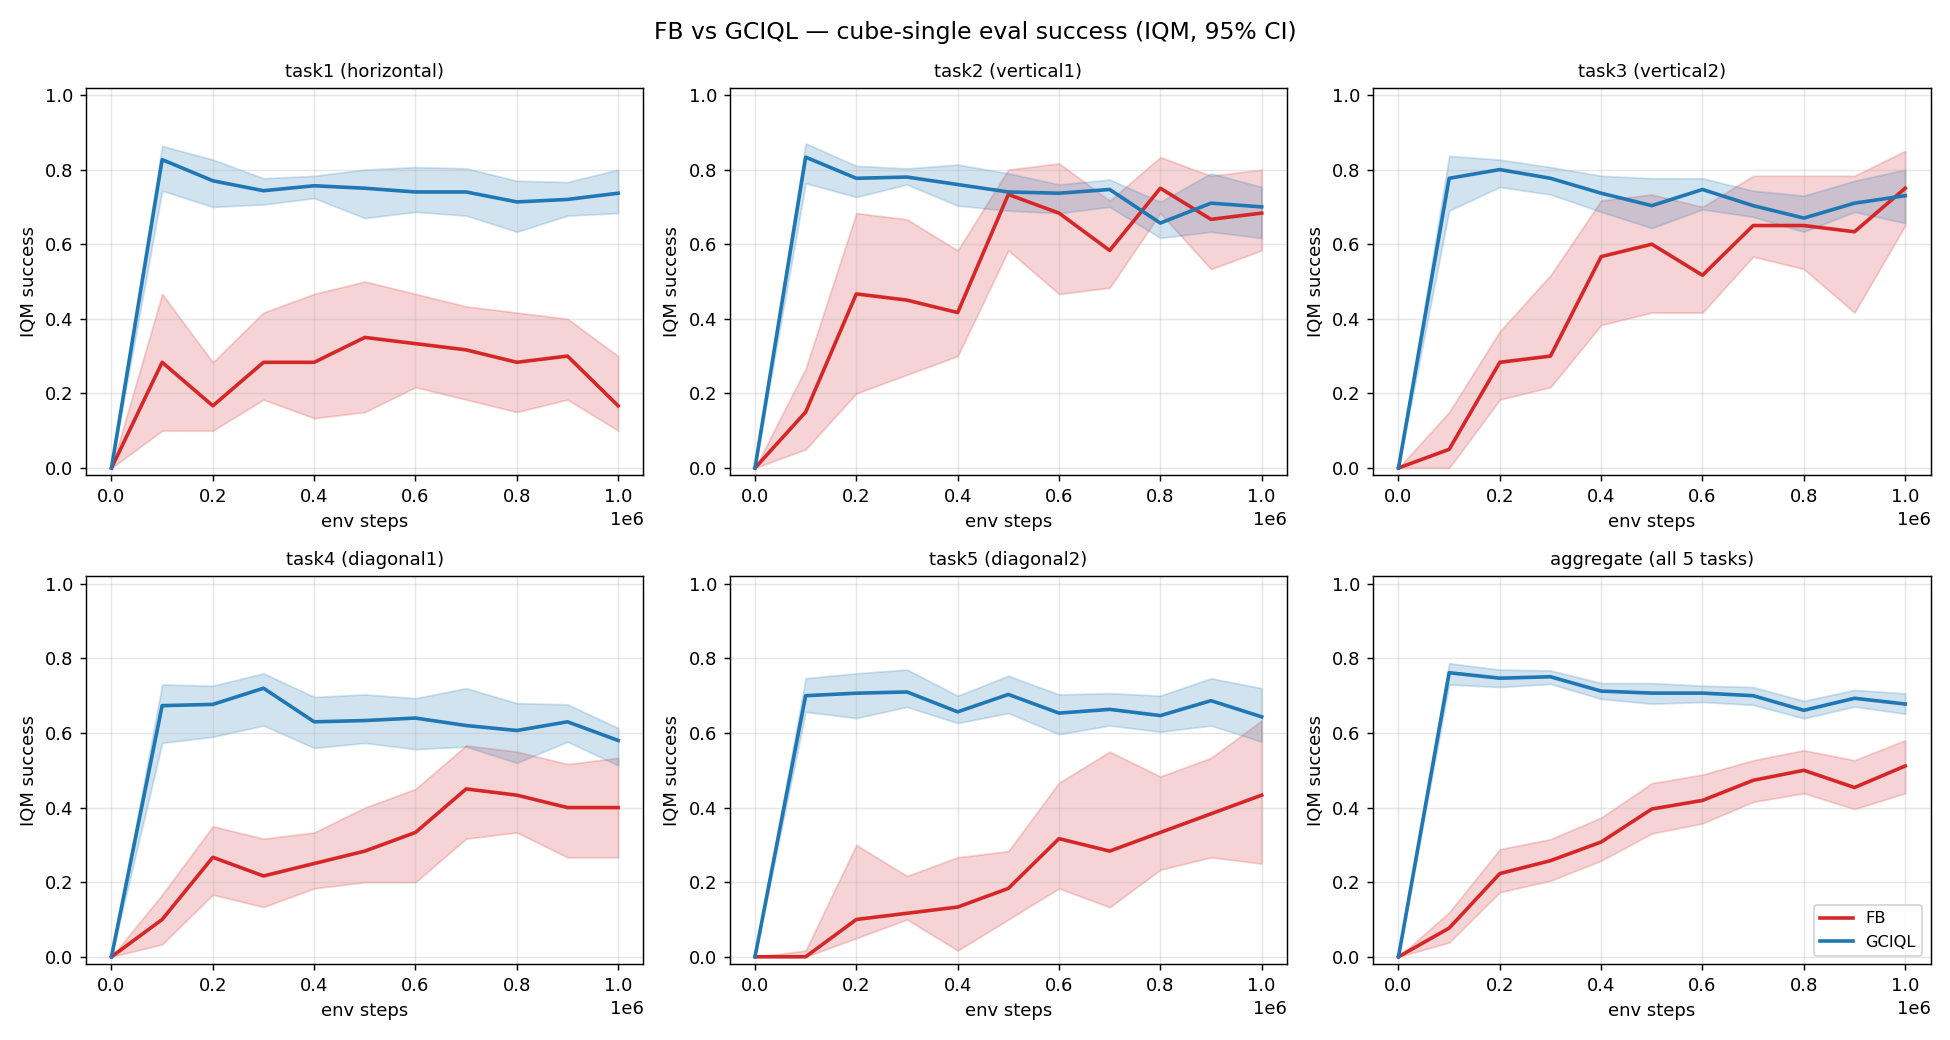
\includegraphics[width=\linewidth]{figures/state/curves_pertask.png}
        \caption{State observations.}
        \label{fig:state-learning-curves-main}
    \end{subfigure}\hfill
    \begin{subfigure}{0.49\linewidth}
        \centering
        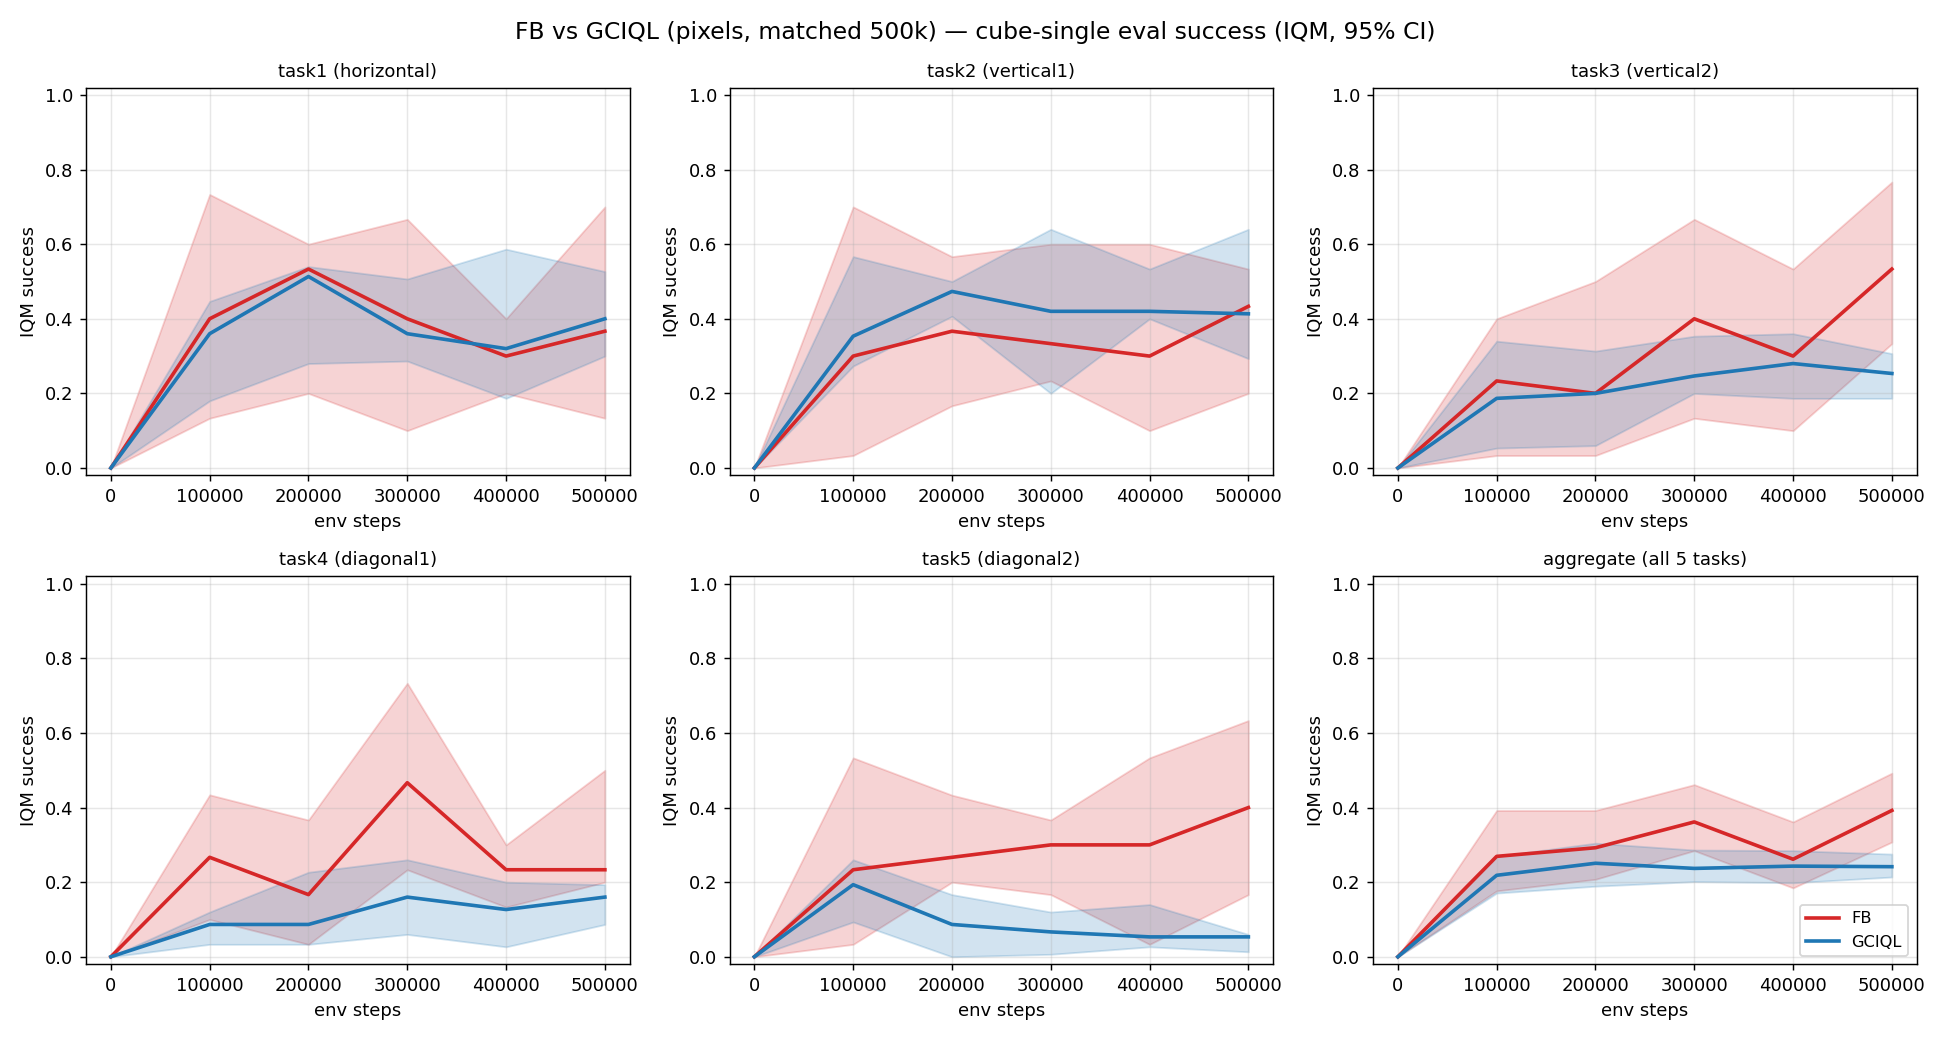
\includegraphics[width=\linewidth]{figures/pixel/pixel_curves_pertask.png}
        \caption{Pixel observations.}
        \label{fig:pixel-learning-curves-main}
    \end{subfigure}
    \caption{Performance reversal across observation regimes. In the state setting, GCIQL reaches a higher aggregate success and a faster plateau. In the pixel setting, FB+FlowBC is at or above GCIQL on the aggregate and on most tasks at the matched $500$k-step budget. Curves report IQM success over seeds with 95\% confidence intervals.}
    \label{fig:ranking-reversal}
\end{figure}

\begin{table}[H]
\centering
\small
\caption{Aggregate success summary across observation regimes. The state setting favors GCIQL, while the pixel setting favors FB at the matched budget. This reversal motivates a representation-level diagnosis rather than a broad claim that FB is intrinsically weak on manipulation.}
\label{tab:aggregate-reversal}
\vspace{0.25em}
\begin{tabular}{lcc}
\toprule
\textbf{Observation regime} & \textbf{FB+FlowBC} & \textbf{GCIQL} \\
\midrule
State, final aggregate success & $0.500$ & $\mathbf{0.683}$ \\
Pixel, matched $500$k IQM success & $\mathbf{0.407}$ & $0.241$ \\
\bottomrule
\end{tabular}
\end{table}

\takeaway{FB's weakness in the state setting is not a dataset-wide impossibility or an intrinsic failure of the FB factorization. The same method class recovers under a different observation encoder.}

\FloatBarrier
\subsection{Finding 2: The relevant failure mode is transport, not reaching or support}
\label{sec:transport-and-support}

The performance gap should not be interpreted as a generic inability to interact with the cube. In both regimes, the hard phase is final transport: policies reach and secure the cube more often than they complete placement. Moreover, the available support diagnostics do not support a simple off-distribution explanation.

\begin{figure}[H]
    \centering
    \begin{subfigure}{0.49\linewidth}
        \centering
        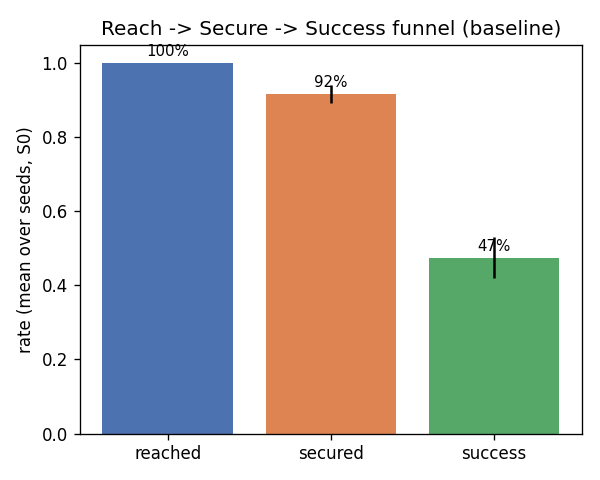
\includegraphics[width=0.88\linewidth]{figures/state/funnel.png}
        \caption{State phase funnel.}
        \label{fig:state-funnel-main}
    \end{subfigure}\hfill
    \begin{subfigure}{0.49\linewidth}
        \centering
        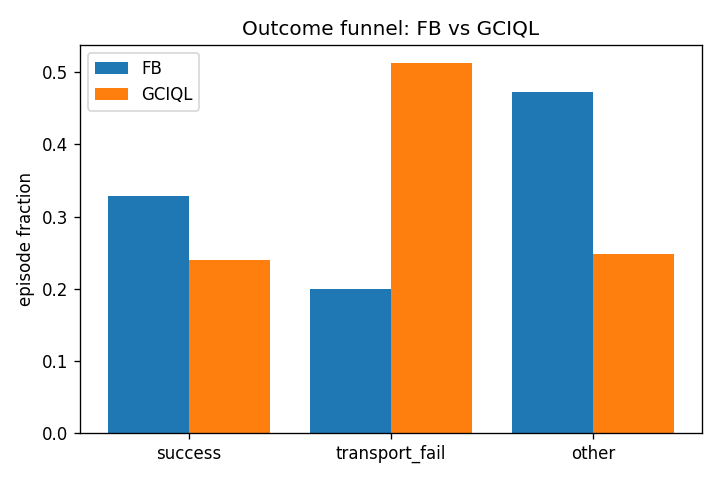
\includegraphics[width=0.88\linewidth]{figures/pixel/pixel_cmp_funnel.png}
        \caption{Pixel phase funnel.}
        \label{fig:pixel-funnel-main}
    \end{subfigure}
    \caption{The manipulation bottleneck is final transport. In both observation regimes, the largest drop occurs after object interaction begins, so the relevant diagnostic target is the terminal placement phase rather than early reaching.}
    \label{fig:funnel-main}
\end{figure}

\begin{figure}[H]
    \centering
    \begin{subfigure}{0.49\linewidth}
        \centering
        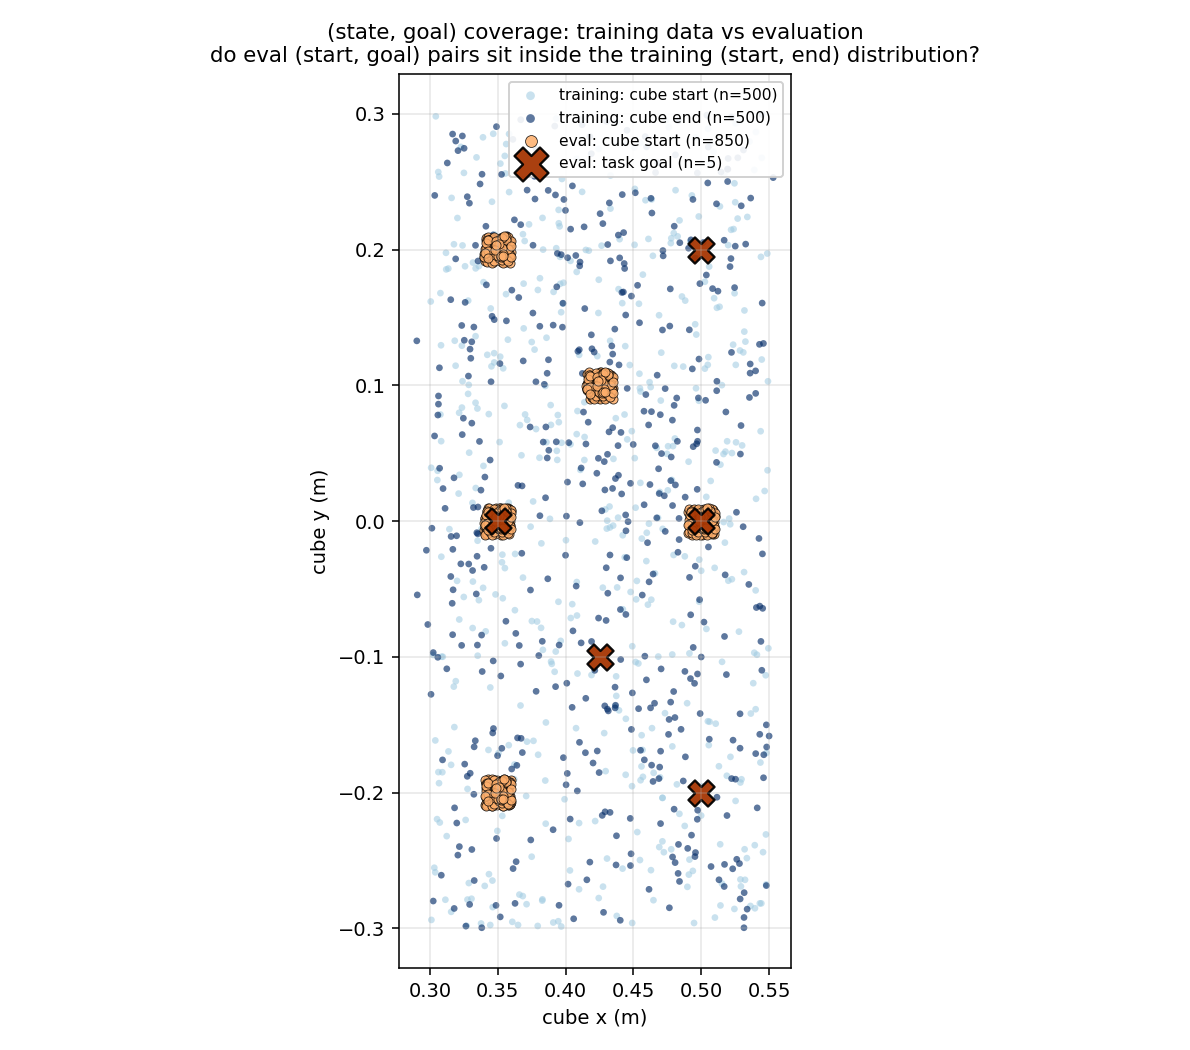
\includegraphics[width=\linewidth]{figures/state/cube_distribution_scatter.png}
        \caption{State evaluation starts/goals relative to training cube positions.}
        \label{fig:state-support-main}
    \end{subfigure}\hfill
    \begin{subfigure}{0.49\linewidth}
        \centering
        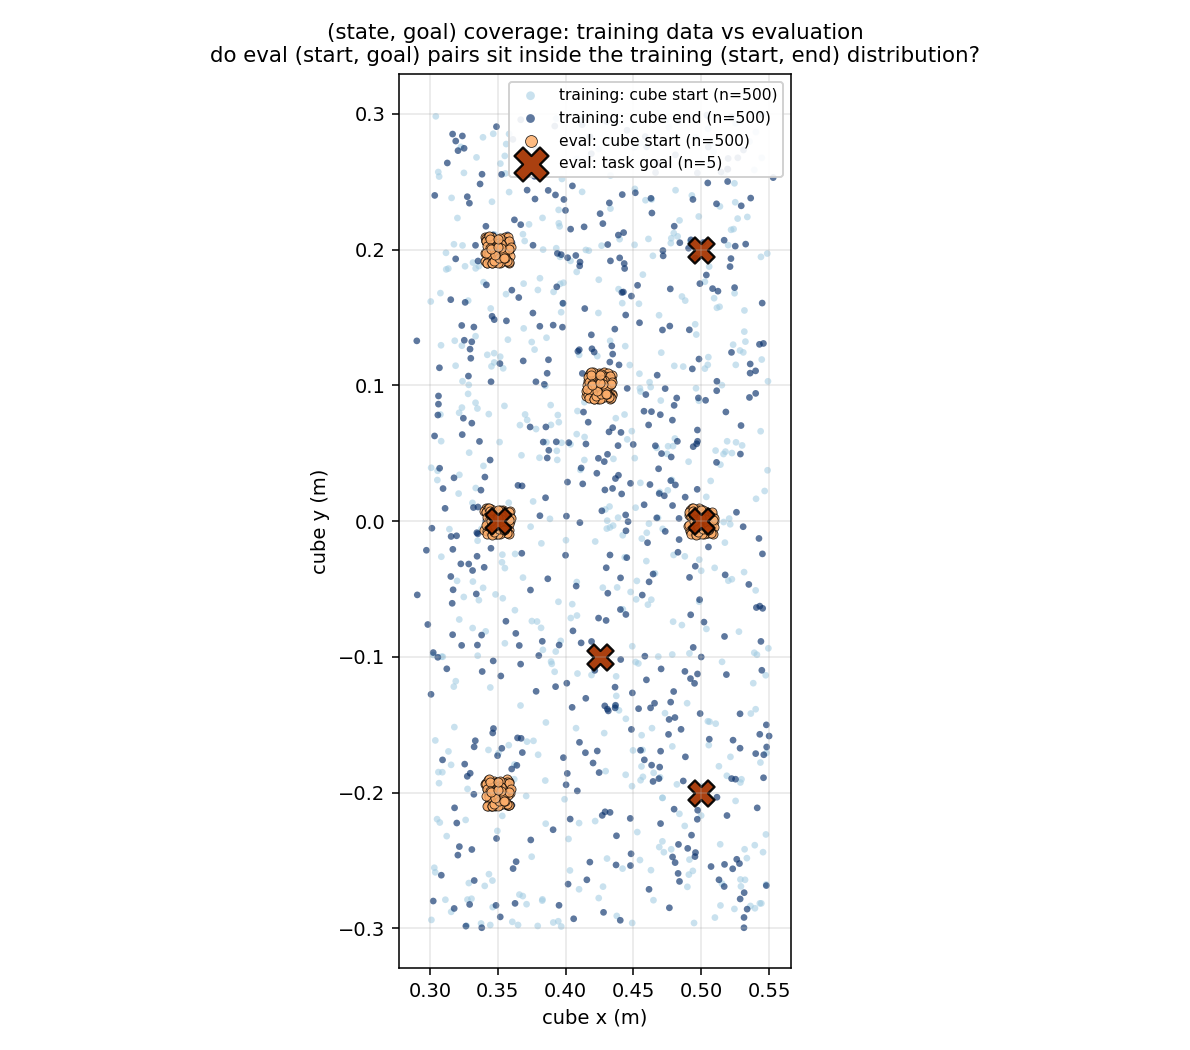
\includegraphics[width=\linewidth]{figures/pixel/pixel_cube_distribution_scatter.png}
        \caption{Pixel evaluation starts/goals relative to training cube positions.}
        \label{fig:pixel-support-main}
    \end{subfigure}
    \caption{Evaluation cube starts and goals lie inside the training cube-position support. Light/dark points indicate training cube starts and endpoints; orange points indicate evaluation starts; dark-red crosses indicate task goals. This does not prove full state-action coverage, but it rules out the simplest object-coordinate OOD explanation.}
    \label{fig:support-main}
\end{figure}

\takeaway{The main phenomenon is not early interaction failure or obvious object-coordinate OOD behavior. The failure is localized to terminal transport, where a useful value function must distinguish successful placement from near-miss.}

\FloatBarrier
\subsection{Finding 3: Terminal resolution in value and $B(s)$ explains the reversal}
\label{sec:terminal-resolution}

The decisive evidence comes from the value and backward-representation probes. Under state observations, FB's value field is weakly aligned with cube-to-goal progress and does not form a stable goal-centered transport basin. Under pixels, FB recovers a more coherent goal-directed value field.

\begin{figure}[H]
    \centering
    \begin{subfigure}{0.49\linewidth}
        \centering
        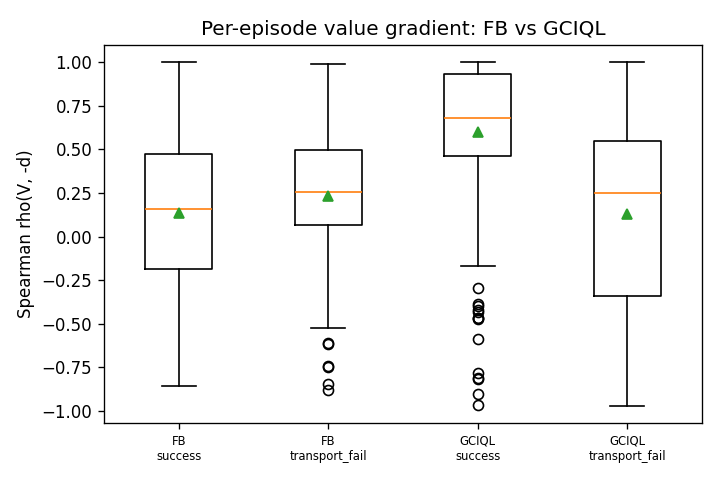
\includegraphics[width=\linewidth]{figures/state/cmp_rho_box.png}
        \caption{State observations.}
        \label{fig:state-rho-main}
    \end{subfigure}\hfill
    \begin{subfigure}{0.49\linewidth}
        \centering
        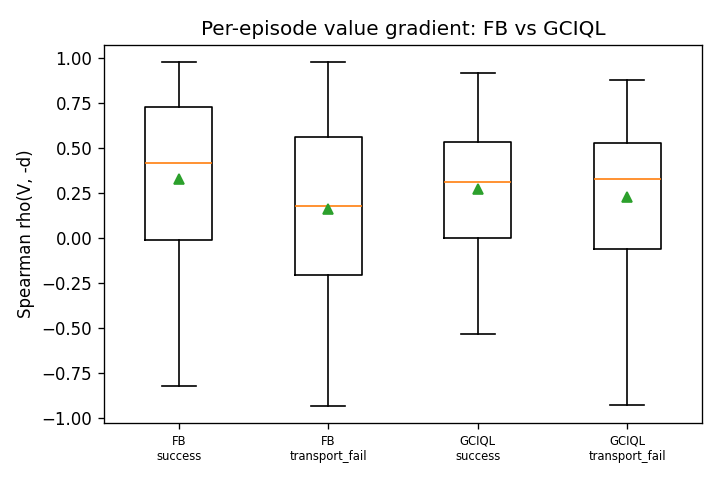
\includegraphics[width=\linewidth]{figures/pixel/pixel_cmp_rho_box.png}
        \caption{Pixel observations.}
        \label{fig:pixel-rho-main}
    \end{subfigure}
    \caption{Value-gradient reversal. We compute per-episode Spearman correlation between extracted value $V(s)=Q_z(s,\pi(s))$ and negative cube-to-goal distance $-d(s,g)$. Under state observations, FB does not separate success and transport-fail cleanly. Under pixels, FB's value is more outcome-discriminating and more aligned with object-to-goal progress.}
    \label{fig:value-gradient-reversal}
\end{figure}

\begin{figure}[H]
    \centering
    \begin{subfigure}{0.49\linewidth}
        \centering
        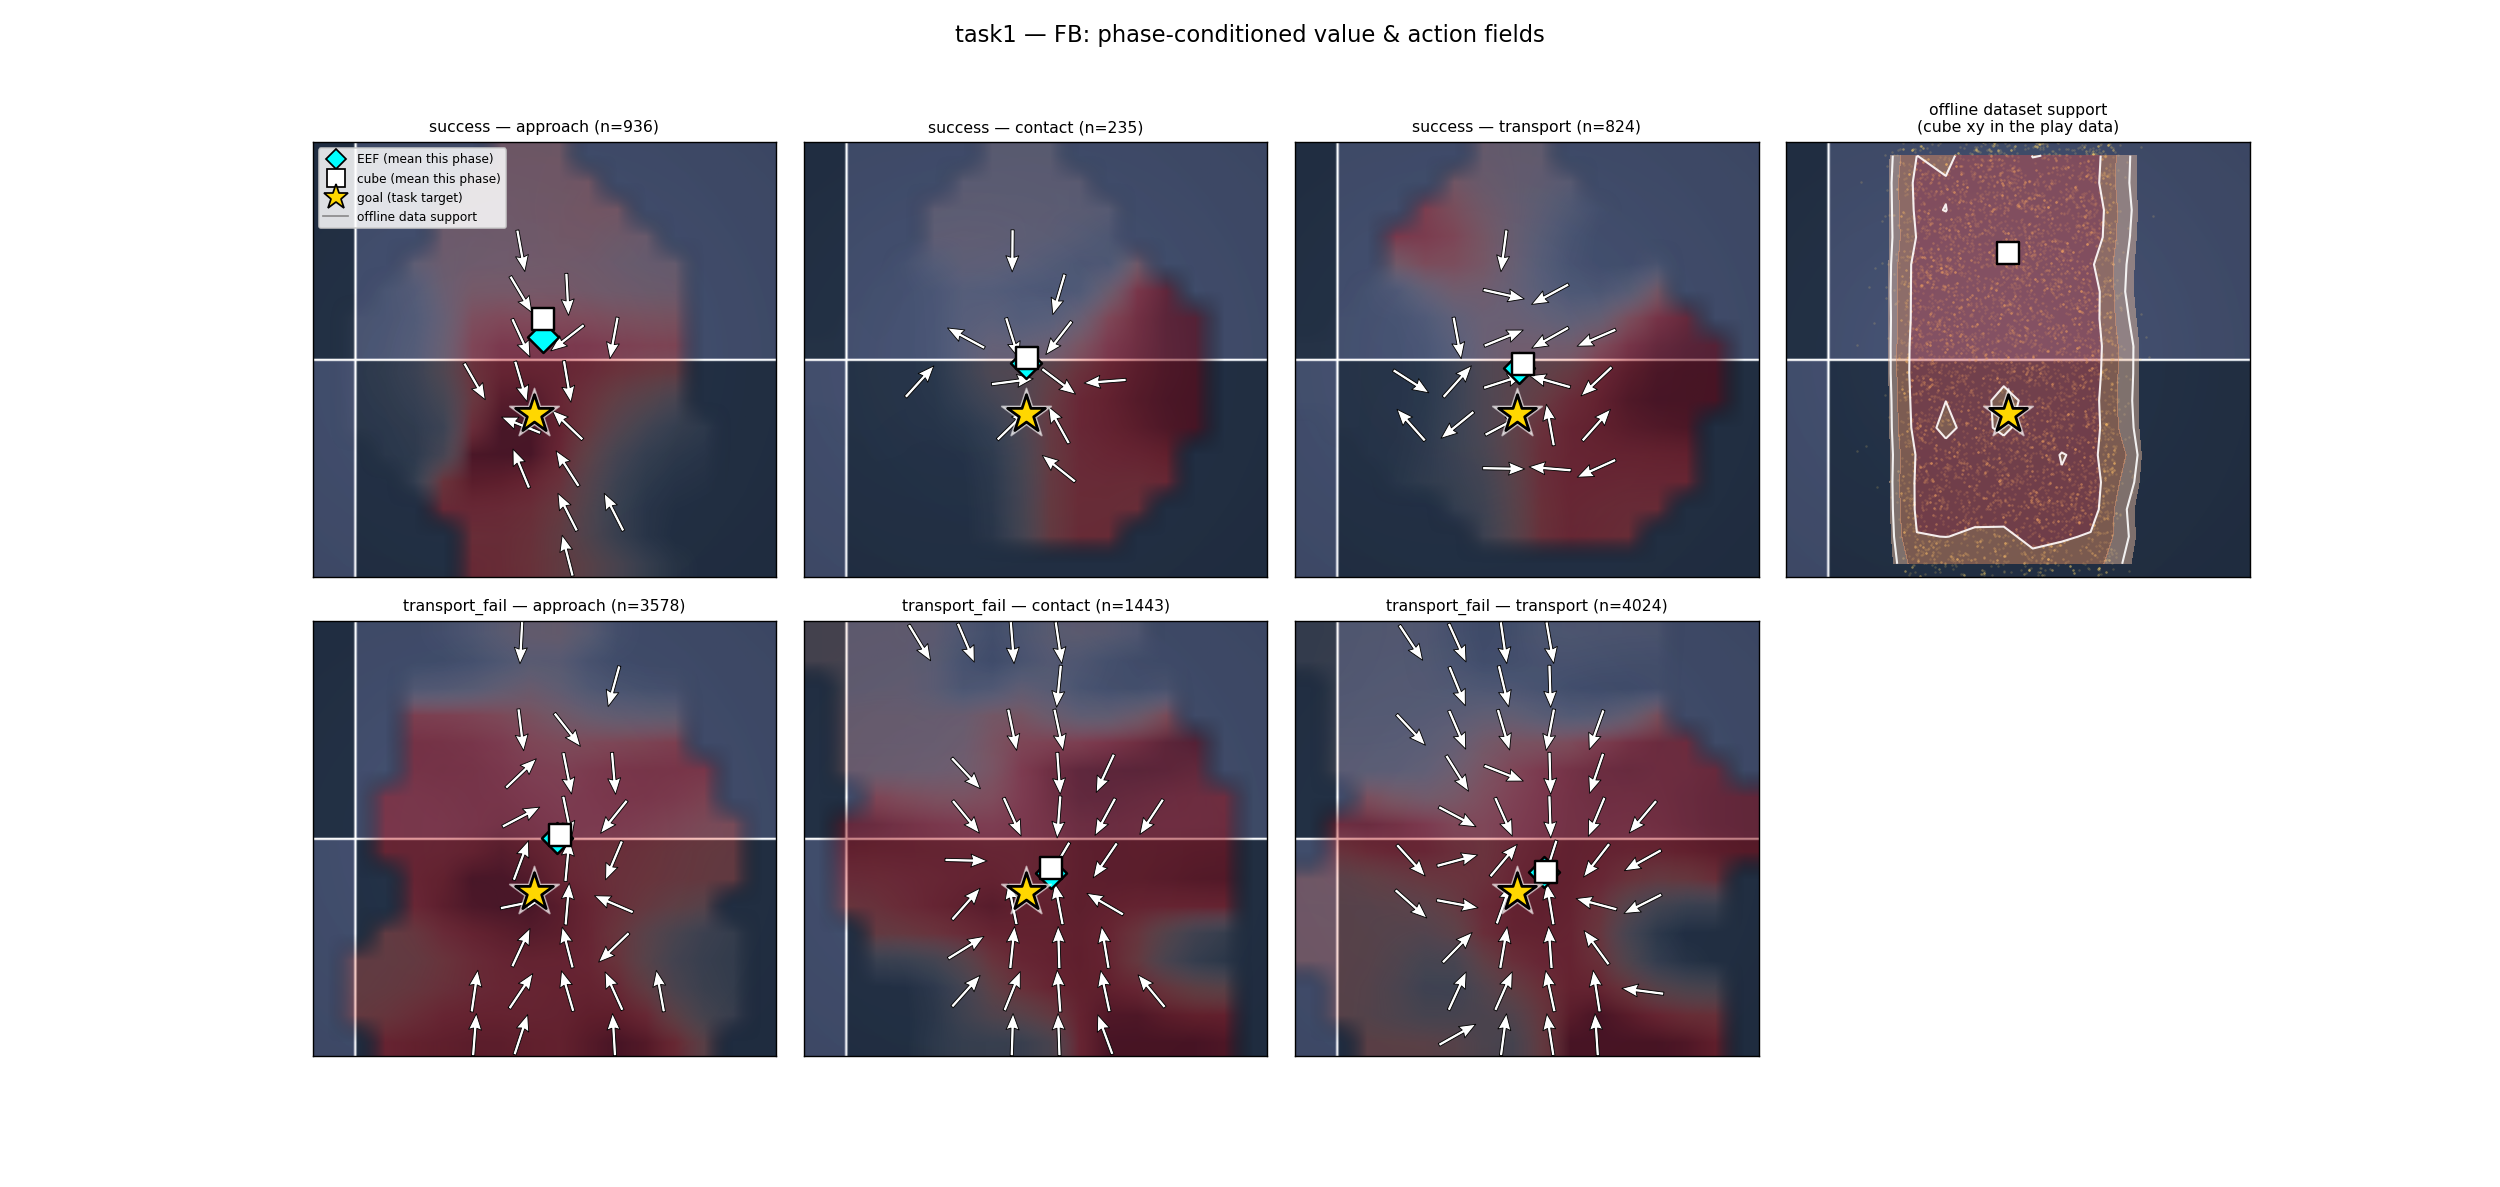
\includegraphics[width=\linewidth]{figures/state/task1__FB.png}
        \caption{State FB, task1.}
        \label{fig:state-field-main}
    \end{subfigure}\hfill
    \begin{subfigure}{0.49\linewidth}
        \centering
        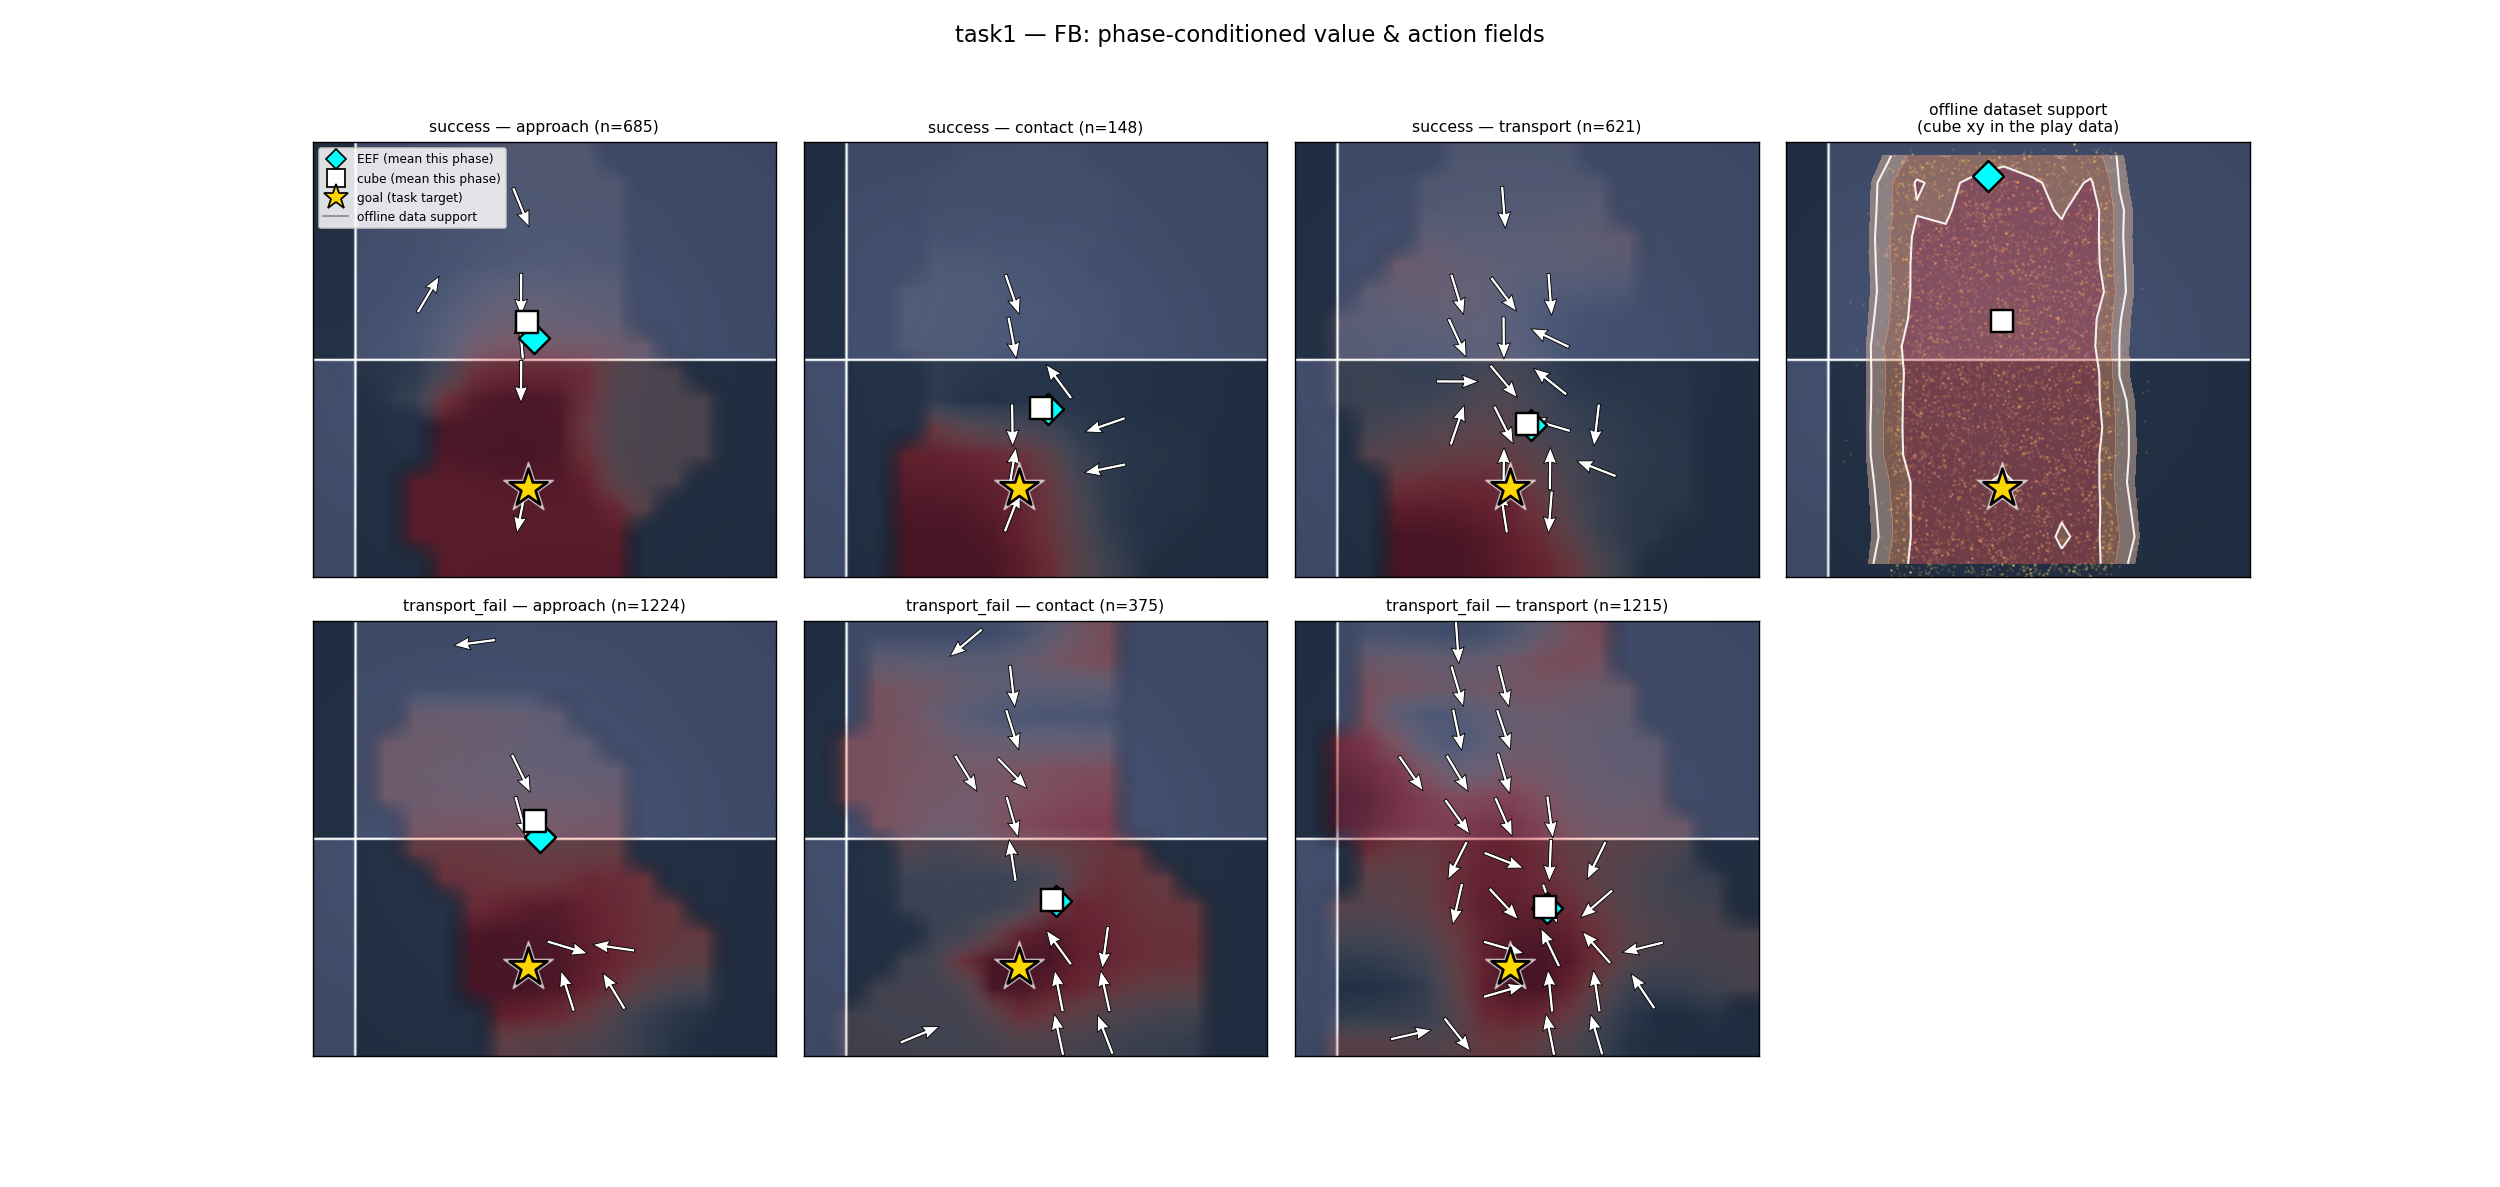
\includegraphics[width=\linewidth]{figures/pixel/pixel_phase_task1__FB.png}
        \caption{Pixel FB, task1.}
        \label{fig:pixel-field-main}
    \end{subfigure}
    \caption{Representative value/action fields for the same task. Each subfigure is a phase-conditioned grid; the diagnostic column is transport. Under state observations, FB lacks a stable goal-centered transport basin. Under pixels, FB forms a sharper goal-directed basin and a more coherent transport action field. Full phase-conditioned atlases are in \Cref{app:state-phase-atlas,app:pixel-phase-atlas}.}
    \label{fig:state-vs-pixel-fields-main}
\end{figure}

The same reversal appears directly in $B(s)$. The state backward map is only weakly predictive of cube-to-goal distance and poorly separates true placements from close near-misses. Under pixels, these quantities improve sharply.

\begin{table}[H]
\centering
\small
\caption{Backward-representation summary. The pixel setting reverses the state-setting bottleneck: $B(s)$ becomes substantially more predictive of cube-to-goal distance and much better at separating true placements from near-misses.}
\label{tab:b-resolution-main}
\vspace{0.25em}
\begin{tabular}{lccc}
\toprule
\textbf{Observation} & \textbf{Top-$k$ \% at Goal} & \textbf{$R^2(B\to d)$} & \textbf{Near-Miss Acc.} \\
\midrule
State & $0.21$ & $0.39$ & $0.67$ \\
Pixel & $0.59$ & $0.76$ & $0.93$ \\
\bottomrule
\end{tabular}
\end{table}

\takeaway{The central mechanism is terminal resolution. State FB fails when $B(s)$ is too coarse near the terminal set; pixel FB recovers when the representation pipeline makes $B(s)$ sharply distinguish placements from near-misses.}

\section{Synthesis}
\label{sec:synthesis}

\begin{table}[H]
\centering
\small
\caption{Compressed diagnostic summary. The main text retains only the evidence needed to support the central claim; detailed probes and implementation information are moved to the appendix.}
\label{tab:central-synthesis}
\vspace{0.25em}
\begin{tabular}{p{0.27\linewidth}p{0.27\linewidth}p{0.27\linewidth}p{0.12\linewidth}}
\toprule
\textbf{Question} & \textbf{State observations} & \textbf{Pixel observations} & \textbf{Verdict} \\
\midrule
Which method performs better? 
& GCIQL leads: $0.683$ vs.\ FB $0.500$. 
& FB leads: $0.407$ vs.\ GCIQL $0.241$. 
& Reversal. \\

Where is the hard phase? 
& Failure concentrates after reach/secure, during transport. 
& Residual failures also concentrate during transport. 
& Terminal phase. \\

Is this obvious OOD? 
& Evaluation cube starts/goals lie inside training cube-position support. 
& Same object-coordinate support conclusion. 
& Not primary. \\

Does FB value track progress? 
& Weakly; no stable goal-centered basin. 
& More strongly; goal-directed transport field emerges. 
& Reversal. \\

Does $B(s)$ resolve placement? 
& Weakly: $R^2=0.39$, near-miss acc.\ $0.67$. 
& Strongly: $R^2=0.76$, near-miss acc.\ $0.93$. 
& Decisive. \\
\bottomrule
\end{tabular}
\end{table}

FB fails when the learned task representation does not resolve the terminal placement predicate. 
In the state setting, FB reaches object interaction often enough and does not obviously leave the object-coordinate support, but its value field lacks a goal-centered basin and its backward map is too coarse. In the pixel setting, the same method class recovers: value becomes aligned with object-to-goal progress and $B(s)$ sharply separates placements from near-misses.

This has a direct algorithmic implication. 
If we conclude only that FB is weak on manipulation, the natural fix is to replace the factorization or use a stronger actor. 
The cross-regime evidence points elsewhere: the decisive question is whether the representation pipeline gives $B(s)$ enough terminal resolution. 
This suggests that successor-measure methods may remain viable for manipulation when paired with encoders, object-centric structure, or auxiliary objectives that preserve terminal geometry.

\clearpage
\appendix

\section{Detailed Diagnostic Protocol}
\label{app:diagnostic-protocol}

\paragraph{Outcome labels.}
Each rollout is assigned to one terminal outcome: \emph{success}, \emph{transport-fail}, or \emph{other}. For finer analysis, failures are further decomposed into \emph{fail@reach}, \emph{fail@grasp}, and \emph{fail@transport}. The transport label means the policy reached the object-interaction regime but failed to deliver the cube to the final target.

\paragraph{Phase labels.}
Per-step states are assigned to manipulation phases using gripper and lift signals. We use three coarse phases: \emph{approach}, \emph{contact}, and \emph{transport}. This phase conditioning is important because the same cube position can correspond to different full states.

\paragraph{Support metric.}
For rollout states, we compute $\mnn$, the distance to the nearest comparable state in the offline dataset. Higher $\mnn$ means lower dataset support. In pixel experiments, nearest-neighbor support is measured in cube-position space rather than raw image space.

\paragraph{Value-gradient metric.}
We compute Spearman correlation between extracted value $V(s)=Q_z(s,\pi(s))$ and negative cube-to-goal distance $-d(s,g)$. A positive correlation means that value increases as the cube approaches the goal.

\paragraph{Backward-resolution probes.}
We evaluate $B(s)$ with three probes: top-$k$ localization of decoded task latents, ridge regression from $B(s)$ to cube-to-goal distance, and classification of true placements versus close near-misses.

\section{Detailed State-Observation Diagnostics}
\label{app:state-diagnostics}

\subsection{State outcome composition and support}

\begin{figure}[H]
    \centering
    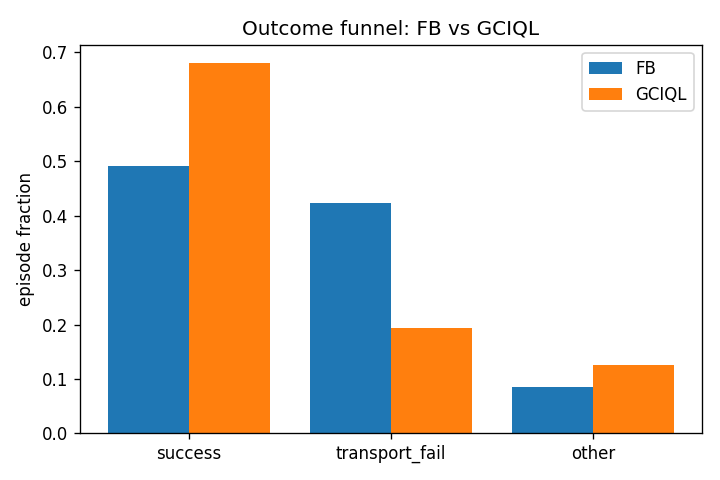
\includegraphics[width=0.55\linewidth]{figures/state/cmp_funnel.png}
    \caption{State observations: final outcome composition for FB and GCIQL. FB loses a larger fraction of episodes during transport, while GCIQL converts more episodes into success on the same data.}
    \label{fig:state-outcome-funnel-app}
\end{figure}

\begin{figure}[H]
    \centering
    \begin{subfigure}{0.48\linewidth}
        \centering
        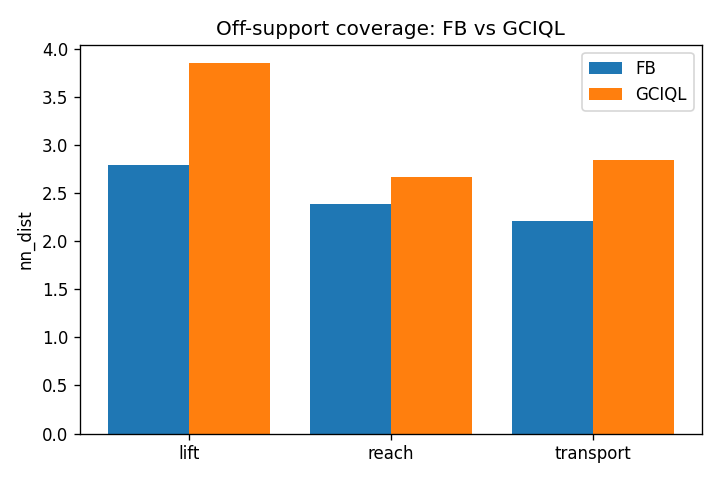
\includegraphics[width=\linewidth]{figures/state/cmp_coverage.png}
        \caption{Method-level support by phase.}
        \label{fig:state-method-coverage-app}
    \end{subfigure}\hfill
    \begin{subfigure}{0.48\linewidth}
        \centering
        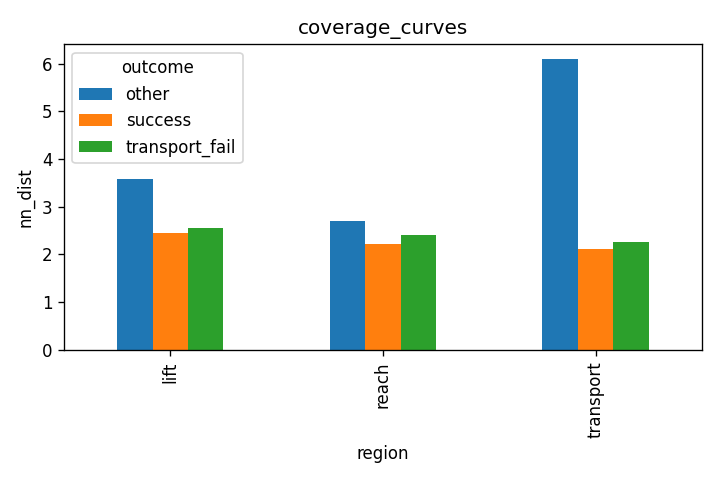
\includegraphics[width=\linewidth]{figures/state/coverage_curves.png}
        \caption{Outcome-conditioned support by phase.}
        \label{fig:state-outcome-coverage-app}
    \end{subfigure}
    \caption{State observations: support diagnostics. Larger $\mnn$ means farther from the empirical dataset manifold. The diagnostic does not support a simple OOD explanation for FB's transport failures.}
    \label{fig:state-coverage-app}
\end{figure}

\begin{table}[H]
\centering
\small
\caption{State observations: dataset-manifold support. If transport failure were an OOD effect, the transport-fail column should be sharply larger, especially in the transport row. It is not.}
\label{tab:state-coverage-app}
\vspace{0.25em}
\begin{tabular}{lcc}
\toprule
\textbf{Region} & \textbf{$\mnn$ (Success)} & \textbf{$\mnn$ (Transport-Fail)} \\
\midrule
reach     & $2.22 \pm 0.74$ & $2.41 \pm 1.29$ \\
lift      & $2.44 \pm 1.73$ & $2.54 \pm 1.41$ \\
transport & $2.12 \pm 0.79$ & $2.25 \pm 1.02$ \\
\bottomrule
\end{tabular}
\end{table}

\subsection{State value and $B$ diagnostics}

\begin{figure}[H]
    \centering
    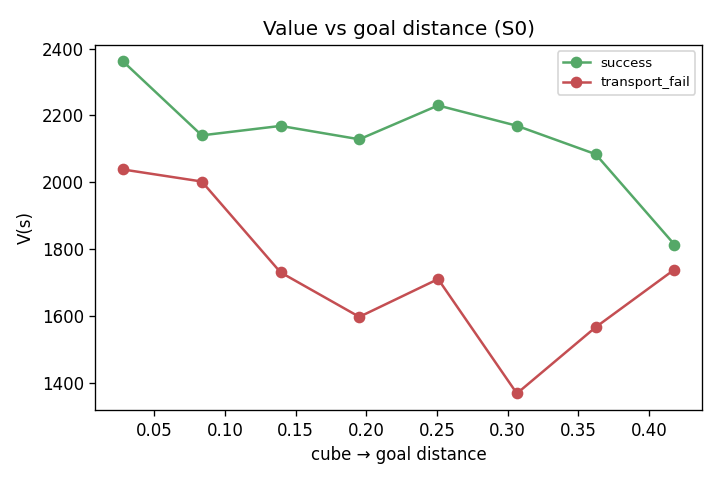
\includegraphics[width=0.60\linewidth]{figures/state/value_vs_dist.png}
    \caption{State observations: raw FB value as a function of cube-to-goal distance under standard initialization $S_0$.}
    \label{fig:fb-raw-value-distance-app}
\end{figure}

\begin{table}[H]
\centering
\small
\caption{State observations: value-landscape gradient for FB. Higher positive $\rho$ means the value ranks states closer to the goal as better.}
\label{tab:state-value-gradient-app}
\vspace{0.25em}
\begin{tabular}{lcc}
\toprule
\textbf{Task} & \textbf{$\rho$ (Success)} & \textbf{$\rho$ (Transport-Fail)} \\
\midrule
task1 & $0.258 \pm 0.264$ & $0.327 \pm 0.358$ \\
task2 & $0.089 \pm 0.341$ & $0.196 \pm 0.249$ \\
task3 & $0.163 \pm 0.332$ & $0.145 \pm 0.213$ \\
task4 & $0.113 \pm 0.664$ & $0.189 \pm 0.466$ \\
task5 & $0.112 \pm 0.568$ & $0.206 \pm 0.446$ \\
\midrule
\textbf{Mean} & $\mathbf{0.147}$ & $\mathbf{0.213}$ \\
\bottomrule
\end{tabular}
\end{table}

\begin{table}[H]
\centering
\small
\caption{State observations: latent sparsity profiling. A sharp goal representation should have low top-$k$ distance and high top-$k$ goal percentage.}
\label{tab:state-sparsity-app}
\vspace{0.25em}
\begin{tabular}{lccc}
\toprule
\textbf{Task} & \textbf{Goal Frac} & \textbf{Top-$k$ $d$} & \textbf{Top-$k$ \% at Goal} \\
\midrule
task1 & $0.0201 \pm 0.0013$ & $0.150 \pm 0.010$ & $0.069 \pm 0.019$ \\
task2 & $0.0208 \pm 0.0017$ & $0.085 \pm 0.006$ & $0.246 \pm 0.036$ \\
task3 & $0.0236 \pm 0.0007$ & $0.094 \pm 0.007$ & $0.278 \pm 0.052$ \\
task4 & $0.0223 \pm 0.0011$ & $0.093 \pm 0.008$ & $0.216 \pm 0.019$ \\
task5 & $0.0240 \pm 0.0015$ & $0.090 \pm 0.011$ & $0.240 \pm 0.042$ \\
\midrule
\textbf{Mean} & $\mathbf{0.0222}$ & $\mathbf{0.103}$ & $\mathbf{0.210}$ \\
\bottomrule
\end{tabular}
\end{table}

\begin{table}[H]
\centering
\small
\caption{State observations: $B$-embedding spatial resolution. Values around $0.665$ near-miss accuracy mean $B$ detects some coarse structure but does not robustly separate success from near-success.}
\label{tab:state-b-resolution-app}
\vspace{0.25em}
\begin{tabular}{lcc}
\toprule
\textbf{Task} & \textbf{Ridge $R^2(B \to d)$} & \textbf{Placed-vs-Near-Miss Acc.} \\
\midrule
task1 & $0.391 \pm 0.024$ & $0.635 \pm 0.023$ \\
task2 & $0.267 \pm 0.025$ & $0.678 \pm 0.016$ \\
task3 & $0.234 \pm 0.016$ & $0.681 \pm 0.016$ \\
task4 & $0.529 \pm 0.005$ & $0.664 \pm 0.018$ \\
task5 & $0.545 \pm 0.024$ & $0.668 \pm 0.014$ \\
\midrule
\textbf{Mean} & $\mathbf{0.393}$ & $\mathbf{0.665}$ \\
\bottomrule
\end{tabular}
\end{table}

\section{Representative Rollout Filmstrips}
\label{app:filmstrips}

\subsection{State observations}

\begin{figure}[H]
    \centering
    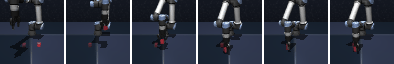
\includegraphics[width=0.98\linewidth]{figures/state/state_filmstrip_task1.png}
    \caption{Representative state rollout, task1.}
\end{figure}

\begin{figure}[H]
    \centering
    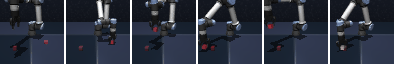
\includegraphics[width=0.98\linewidth]{figures/state/state_filmstrip_task5.png}
    \caption{Representative state rollout, task5.}
\end{figure}

\subsection{Pixel observations}

\begin{figure}[H]
    \centering
    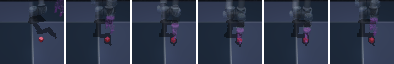
\includegraphics[width=0.98\linewidth]{figures/pixel/pixel_filmstrip_task1.png}
    \caption{Representative pixel rollout, task1.}
\end{figure}

\begin{figure}[H]
    \centering
    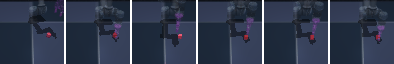
\includegraphics[width=0.98\linewidth]{figures/pixel/pixel_filmstrip_task5.png}
    \caption{Representative pixel rollout, task5.}
\end{figure}

\section{Full Phase-Conditioned Value/Action Atlas: State Observations}
\label{app:state-phase-atlas}

The following figures show the full phase-conditioned value/action fields for all five tasks under state observations. Each method-task figure is a $2\times4$ grid. Rows split terminal outcomes, columns split phases, and the final column shows offline cube-position support.

\begin{figure}[H]
    \centering
    \begin{subfigure}{0.49\linewidth}
        \centering
        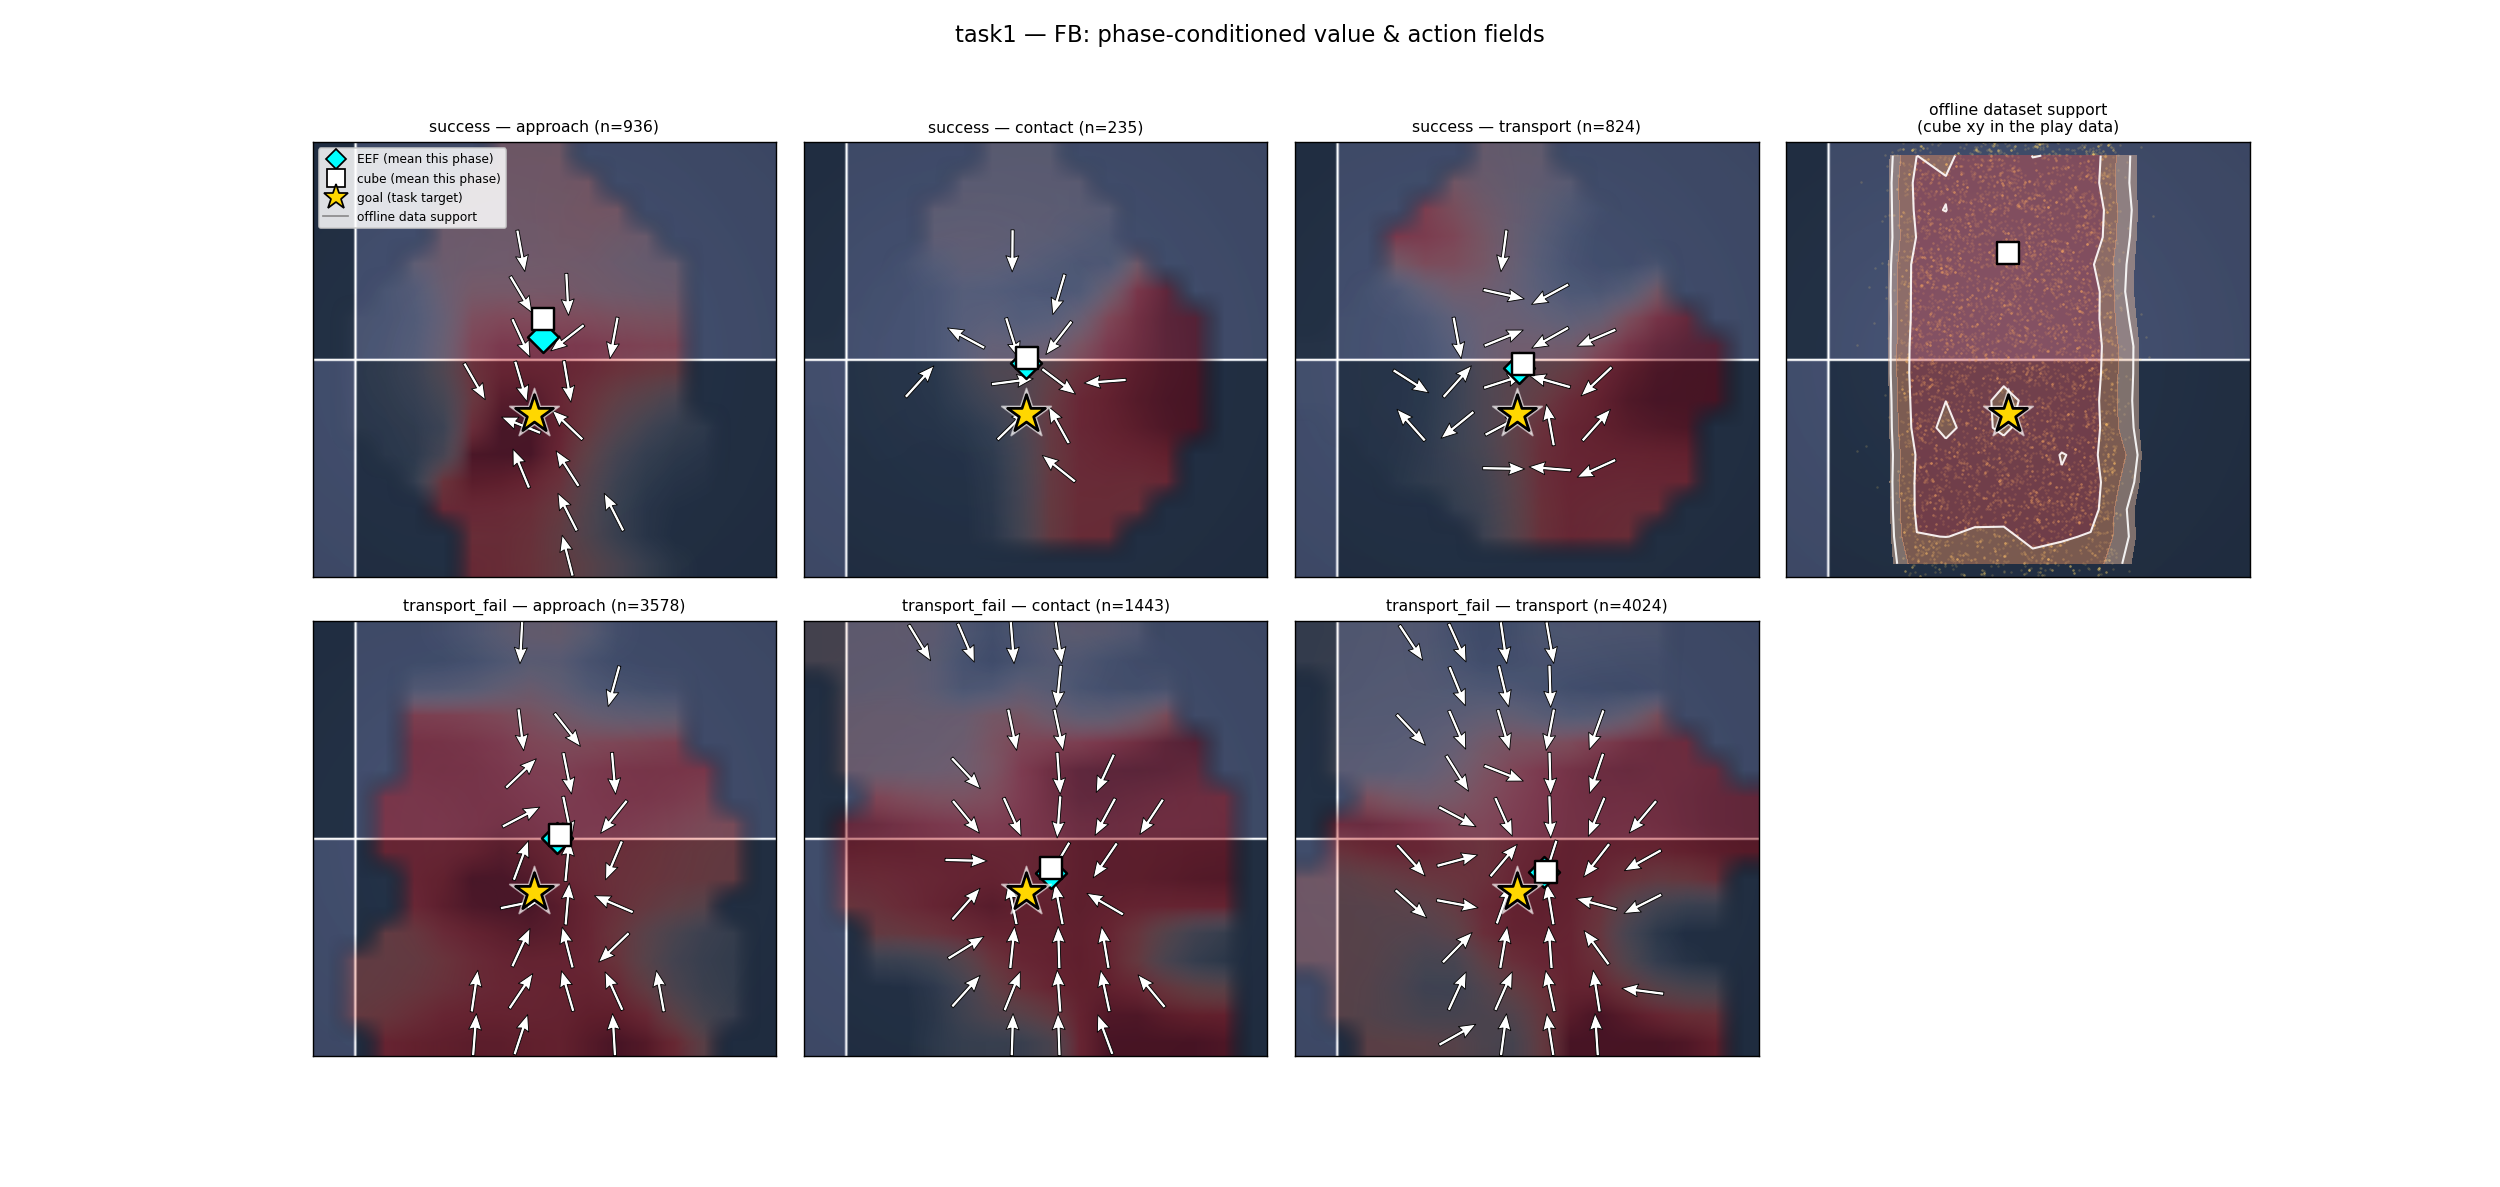
\includegraphics[width=\linewidth]{figures/state/task1__FB.png}
        \caption{task1 -- FB.}
    \end{subfigure}\hfill
    \begin{subfigure}{0.49\linewidth}
        \centering
        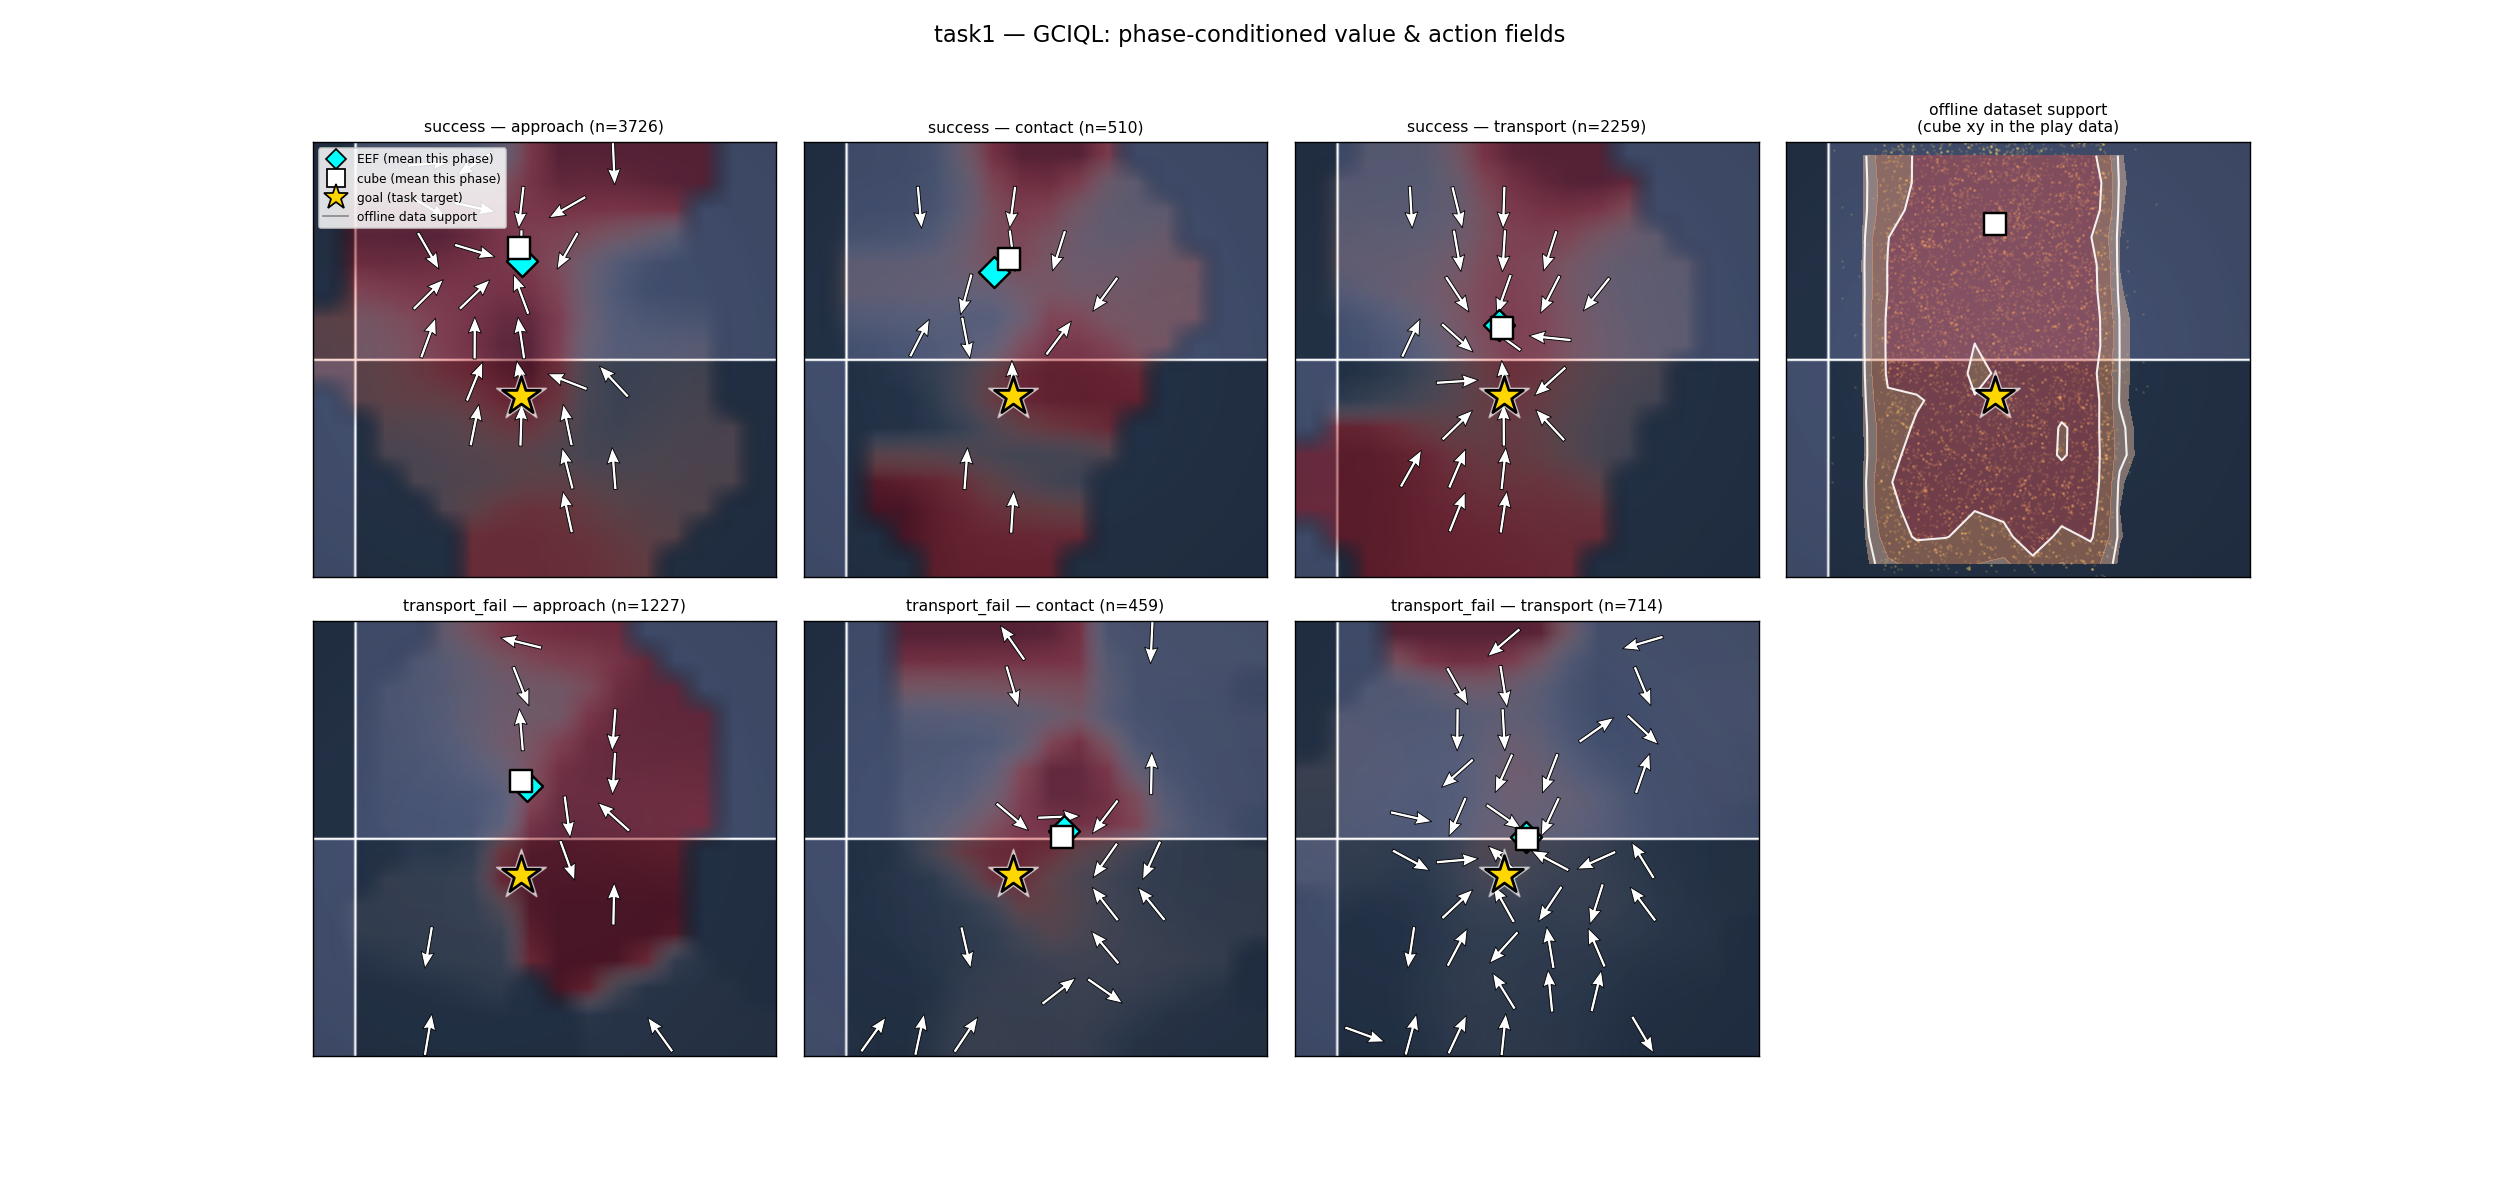
\includegraphics[width=\linewidth]{figures/state/task1__GCIQL.png}
        \caption{task1 -- GCIQL.}
    \end{subfigure}
    \caption{State observations: full phase-conditioned value/action fields for task1.}
\end{figure}

\begin{figure}[H]
    \centering
    \begin{subfigure}{0.49\linewidth}
        \centering
        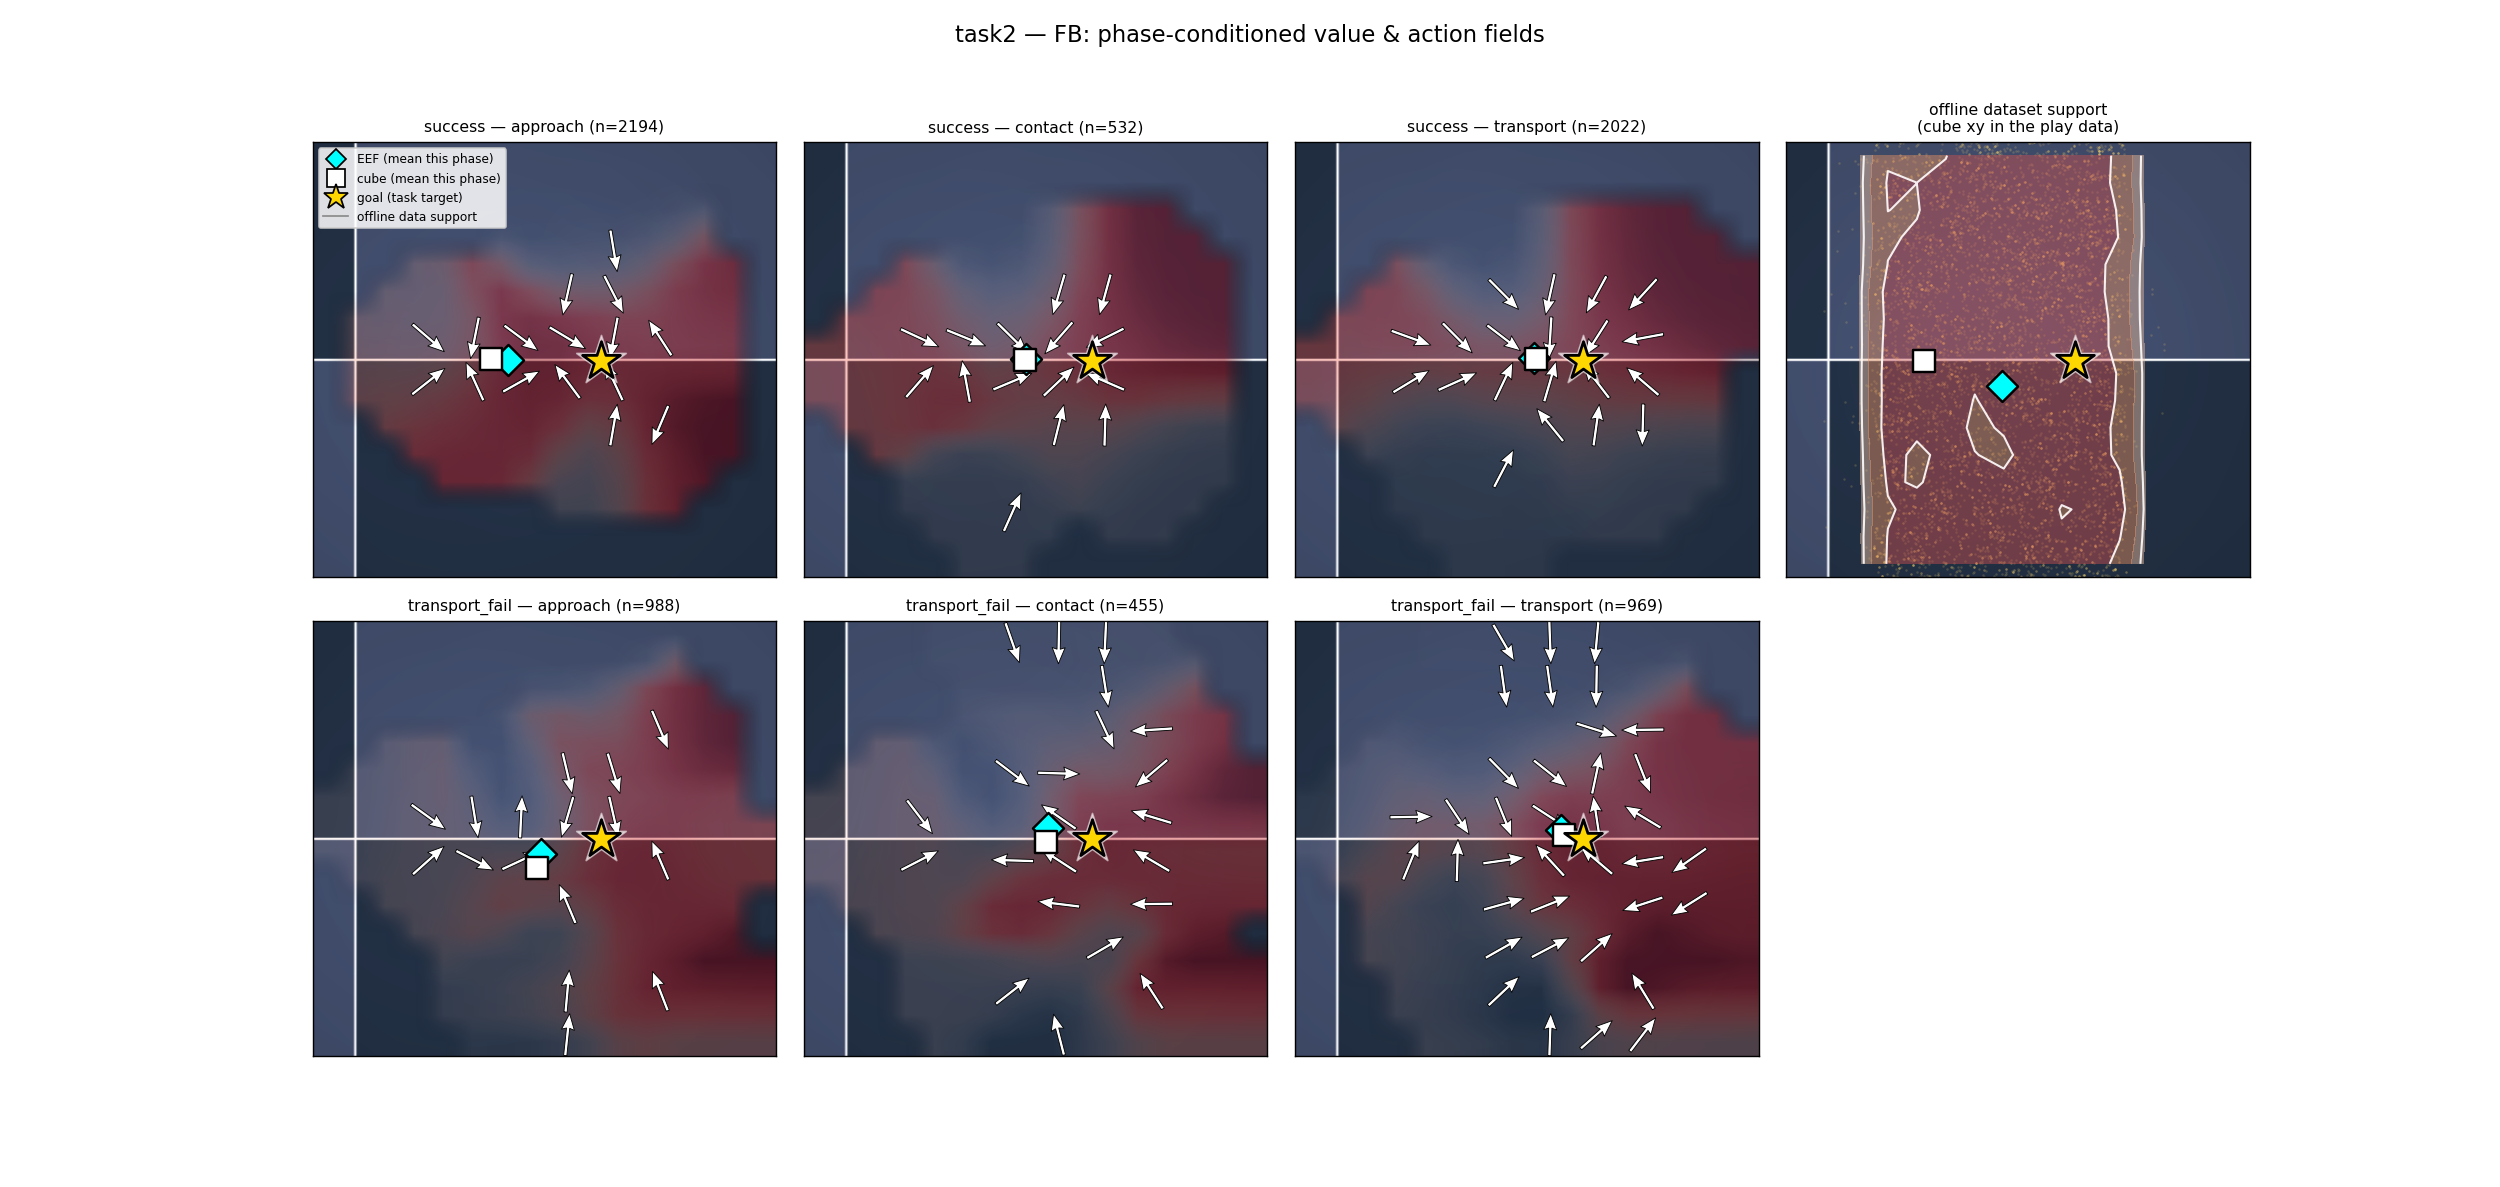
\includegraphics[width=\linewidth]{figures/state/task2__FB.png}
        \caption{task2 -- FB.}
    \end{subfigure}\hfill
    \begin{subfigure}{0.49\linewidth}
        \centering
        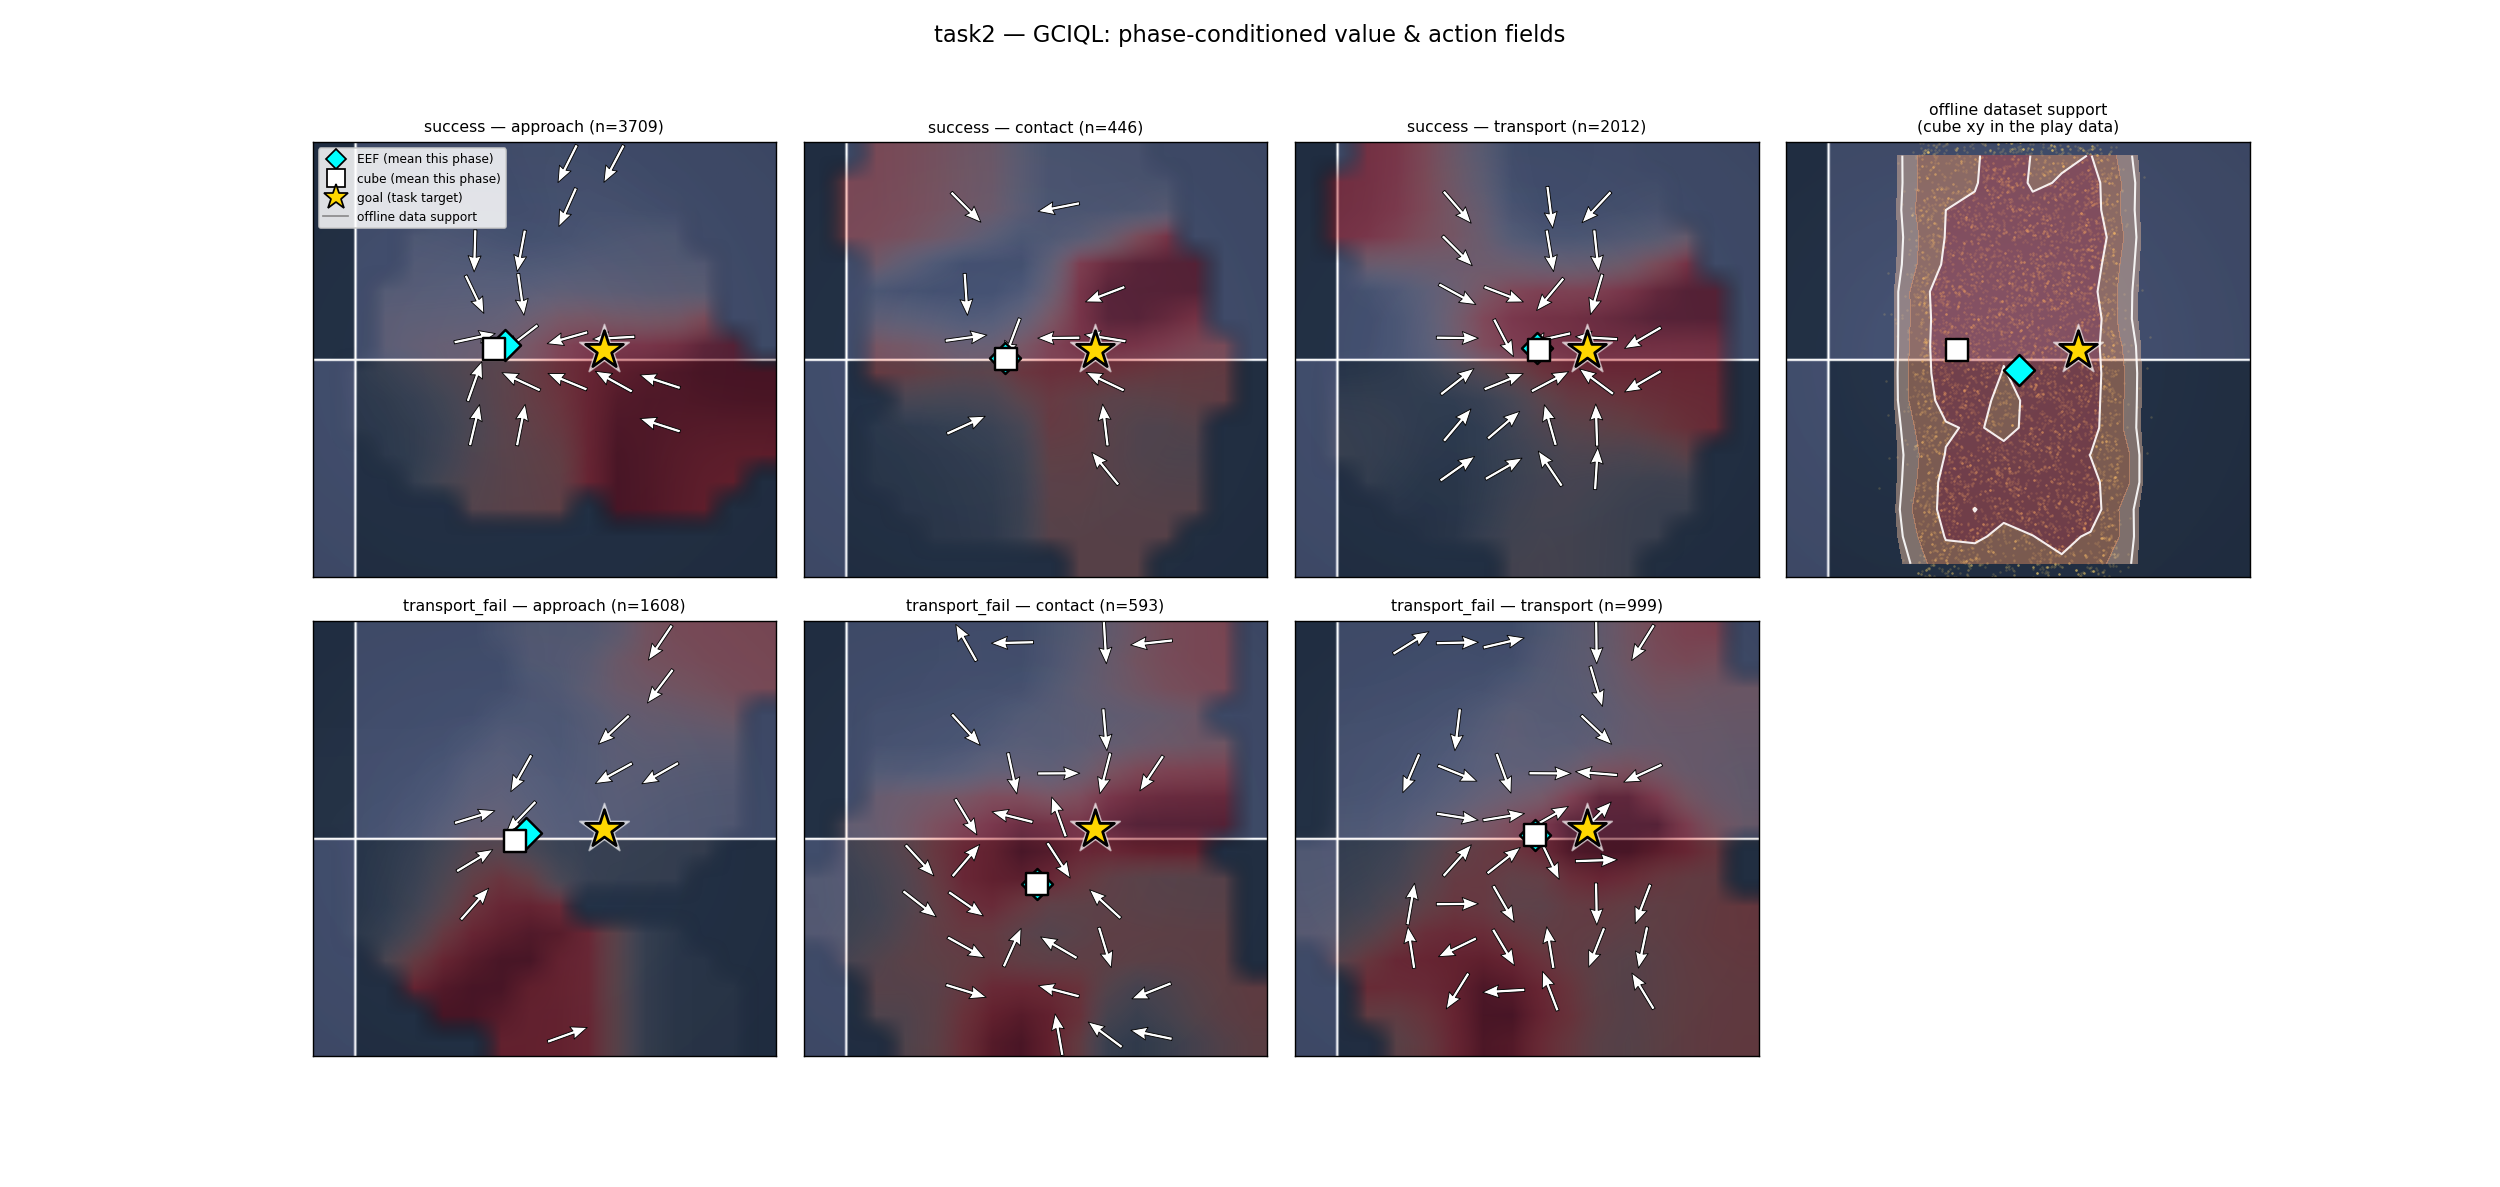
\includegraphics[width=\linewidth]{figures/state/task2__GCIQL.png}
        \caption{task2 -- GCIQL.}
    \end{subfigure}
    \caption{State observations: full phase-conditioned value/action fields for task2.}
\end{figure}

\begin{figure}[H]
    \centering
    \begin{subfigure}{0.49\linewidth}
        \centering
        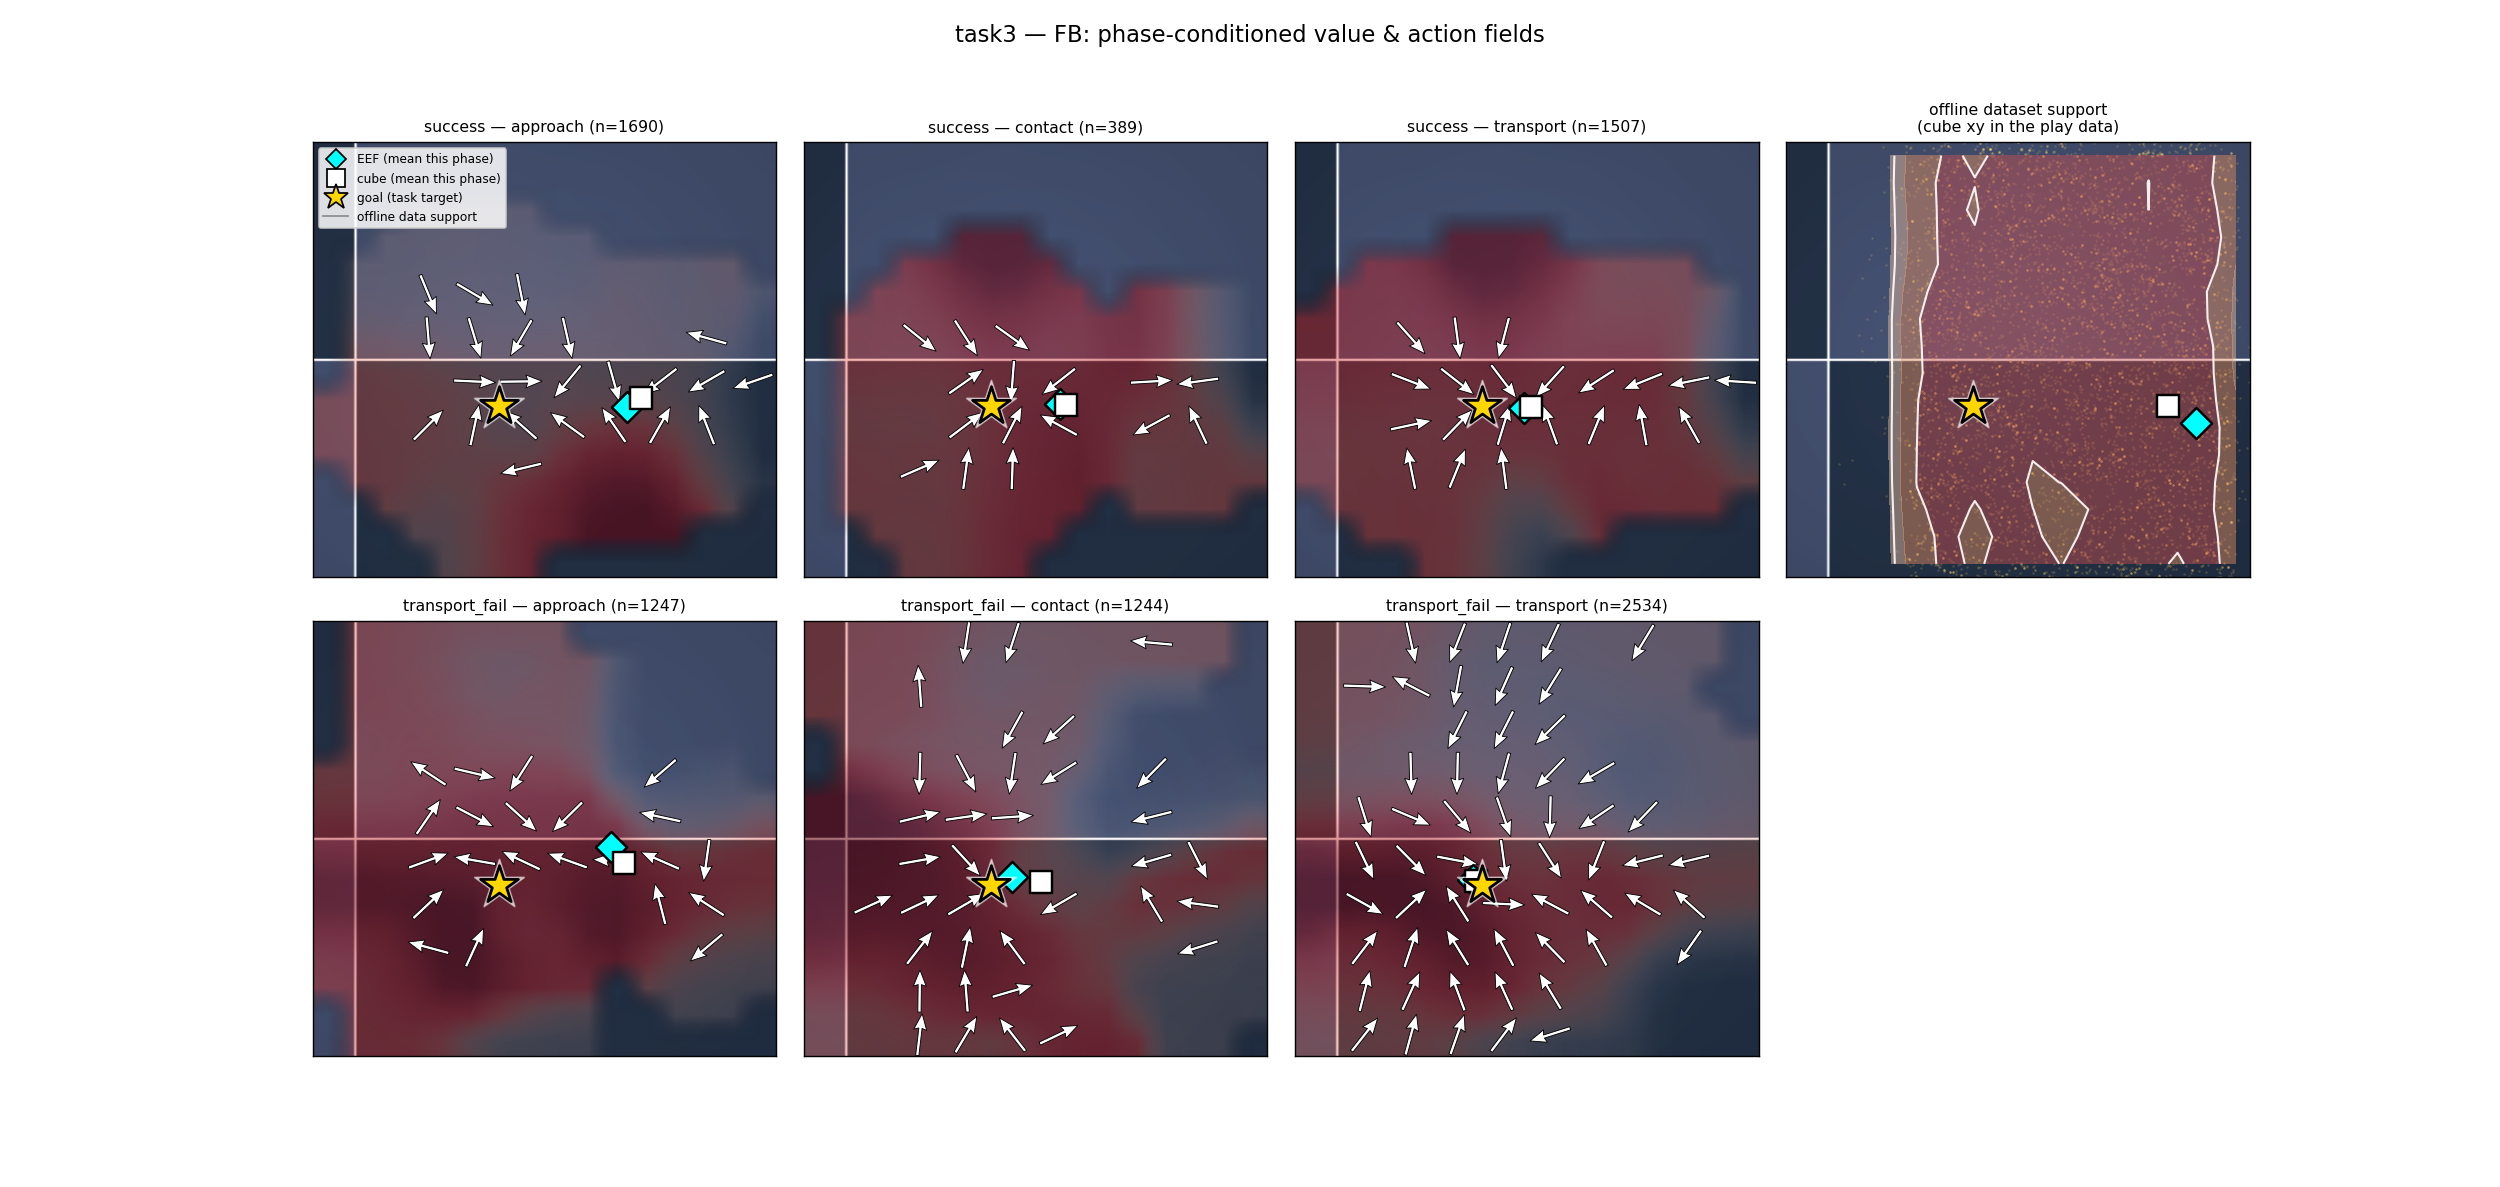
\includegraphics[width=\linewidth]{figures/state/task3__FB.png}
        \caption{task3 -- FB.}
    \end{subfigure}\hfill
    \begin{subfigure}{0.49\linewidth}
        \centering
        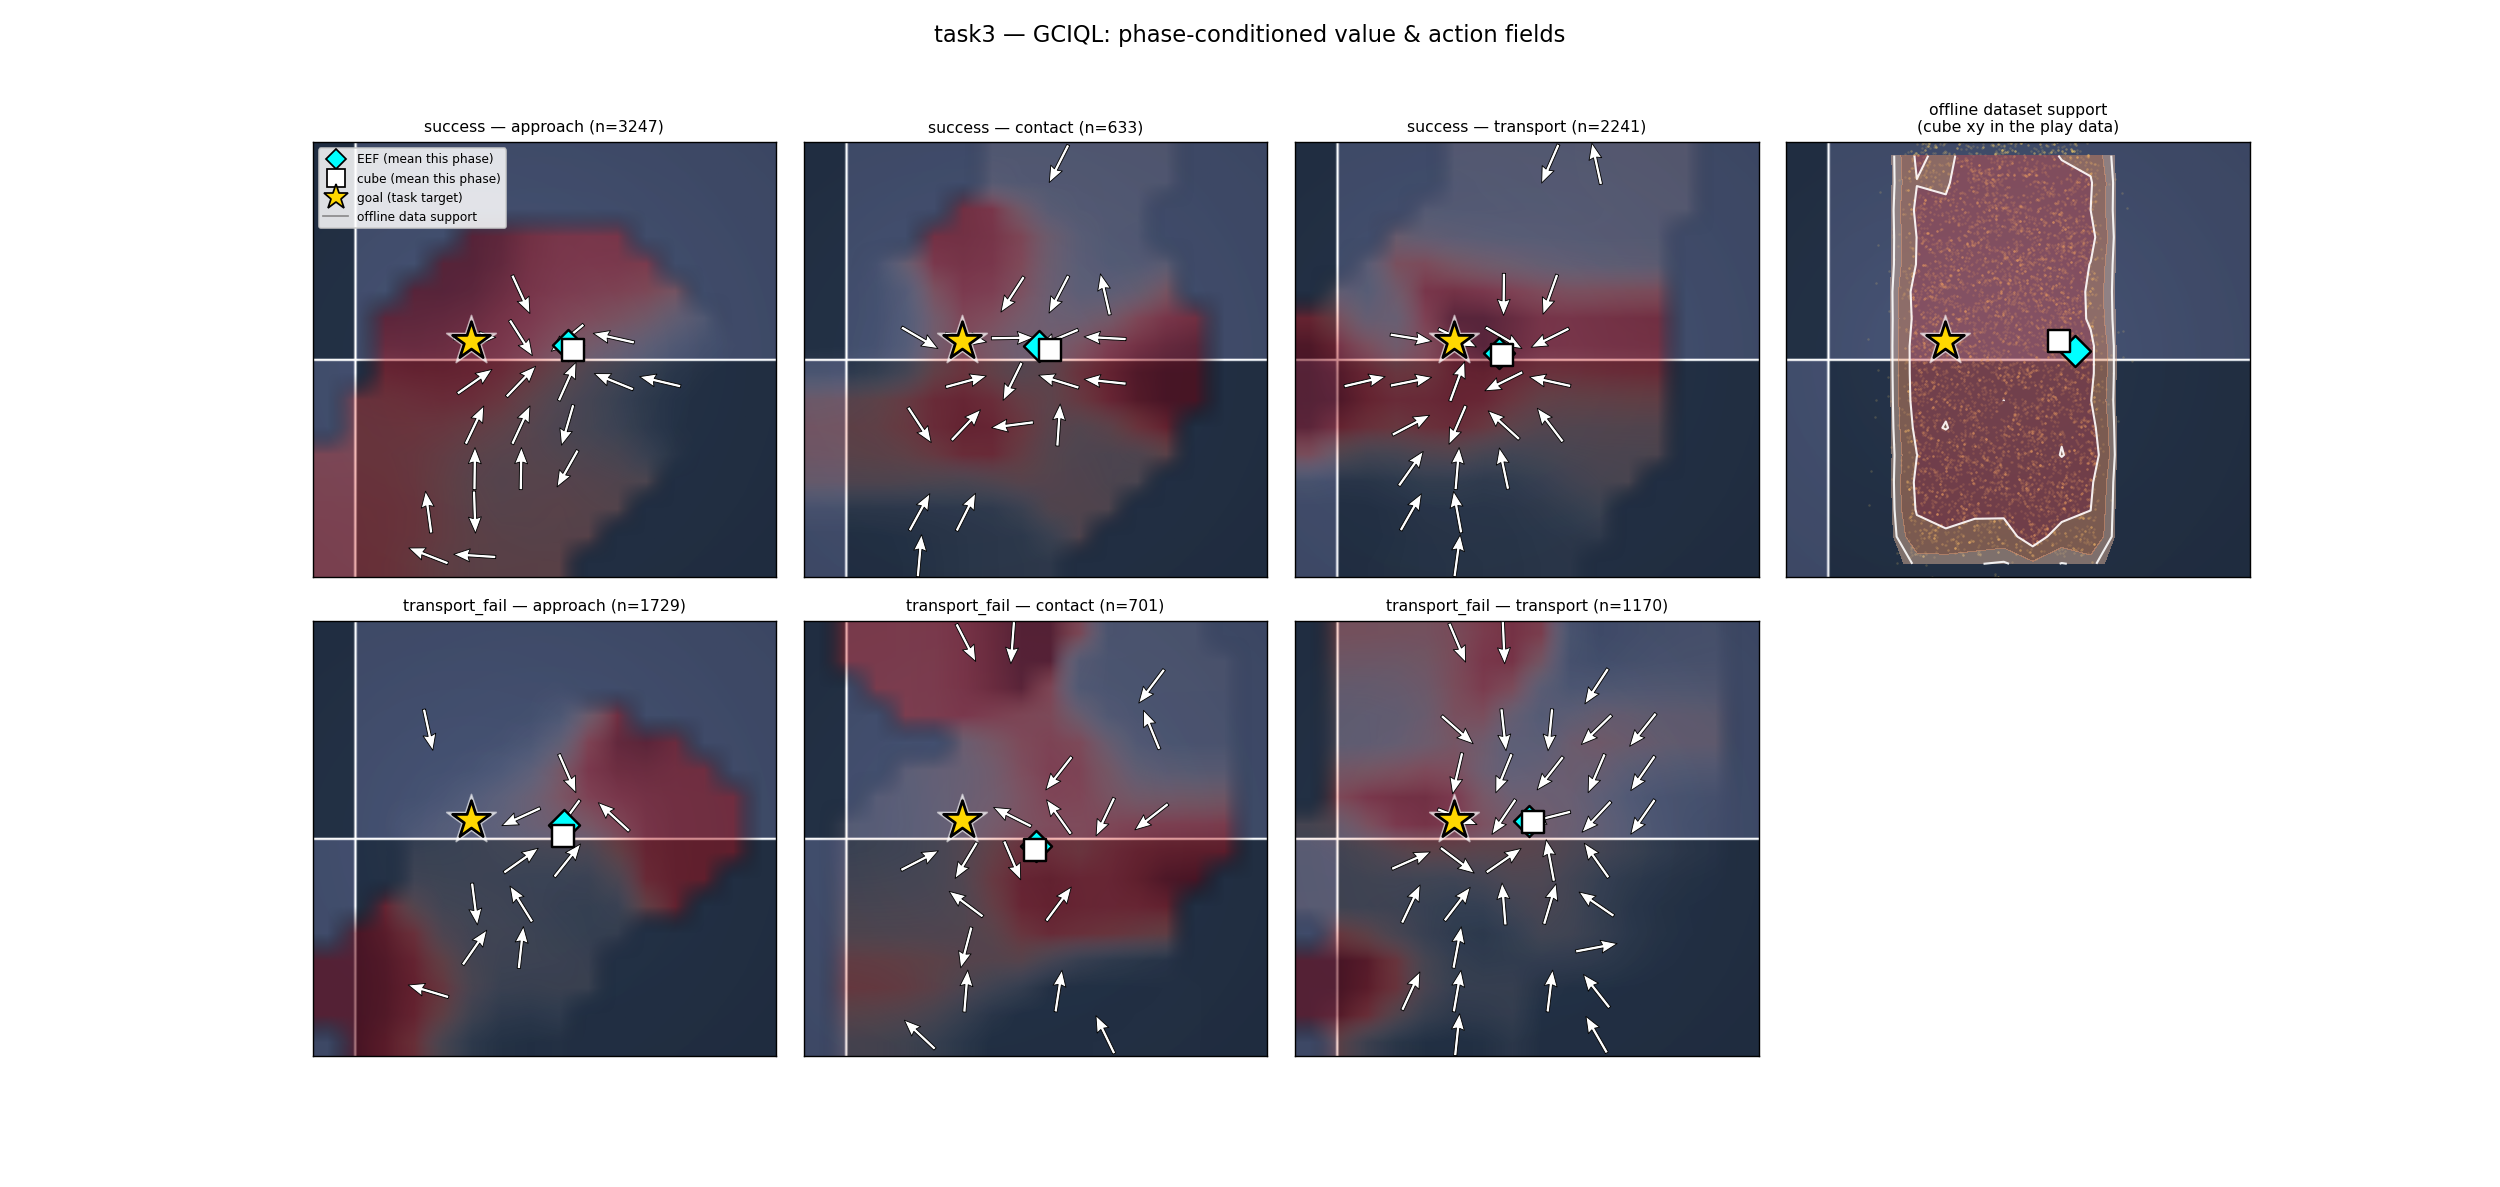
\includegraphics[width=\linewidth]{figures/state/task3__GCIQL.png}
        \caption{task3 -- GCIQL.}
    \end{subfigure}
    \caption{State observations: full phase-conditioned value/action fields for task3.}
\end{figure}

\begin{figure}[H]
    \centering
    \begin{subfigure}{0.49\linewidth}
        \centering
        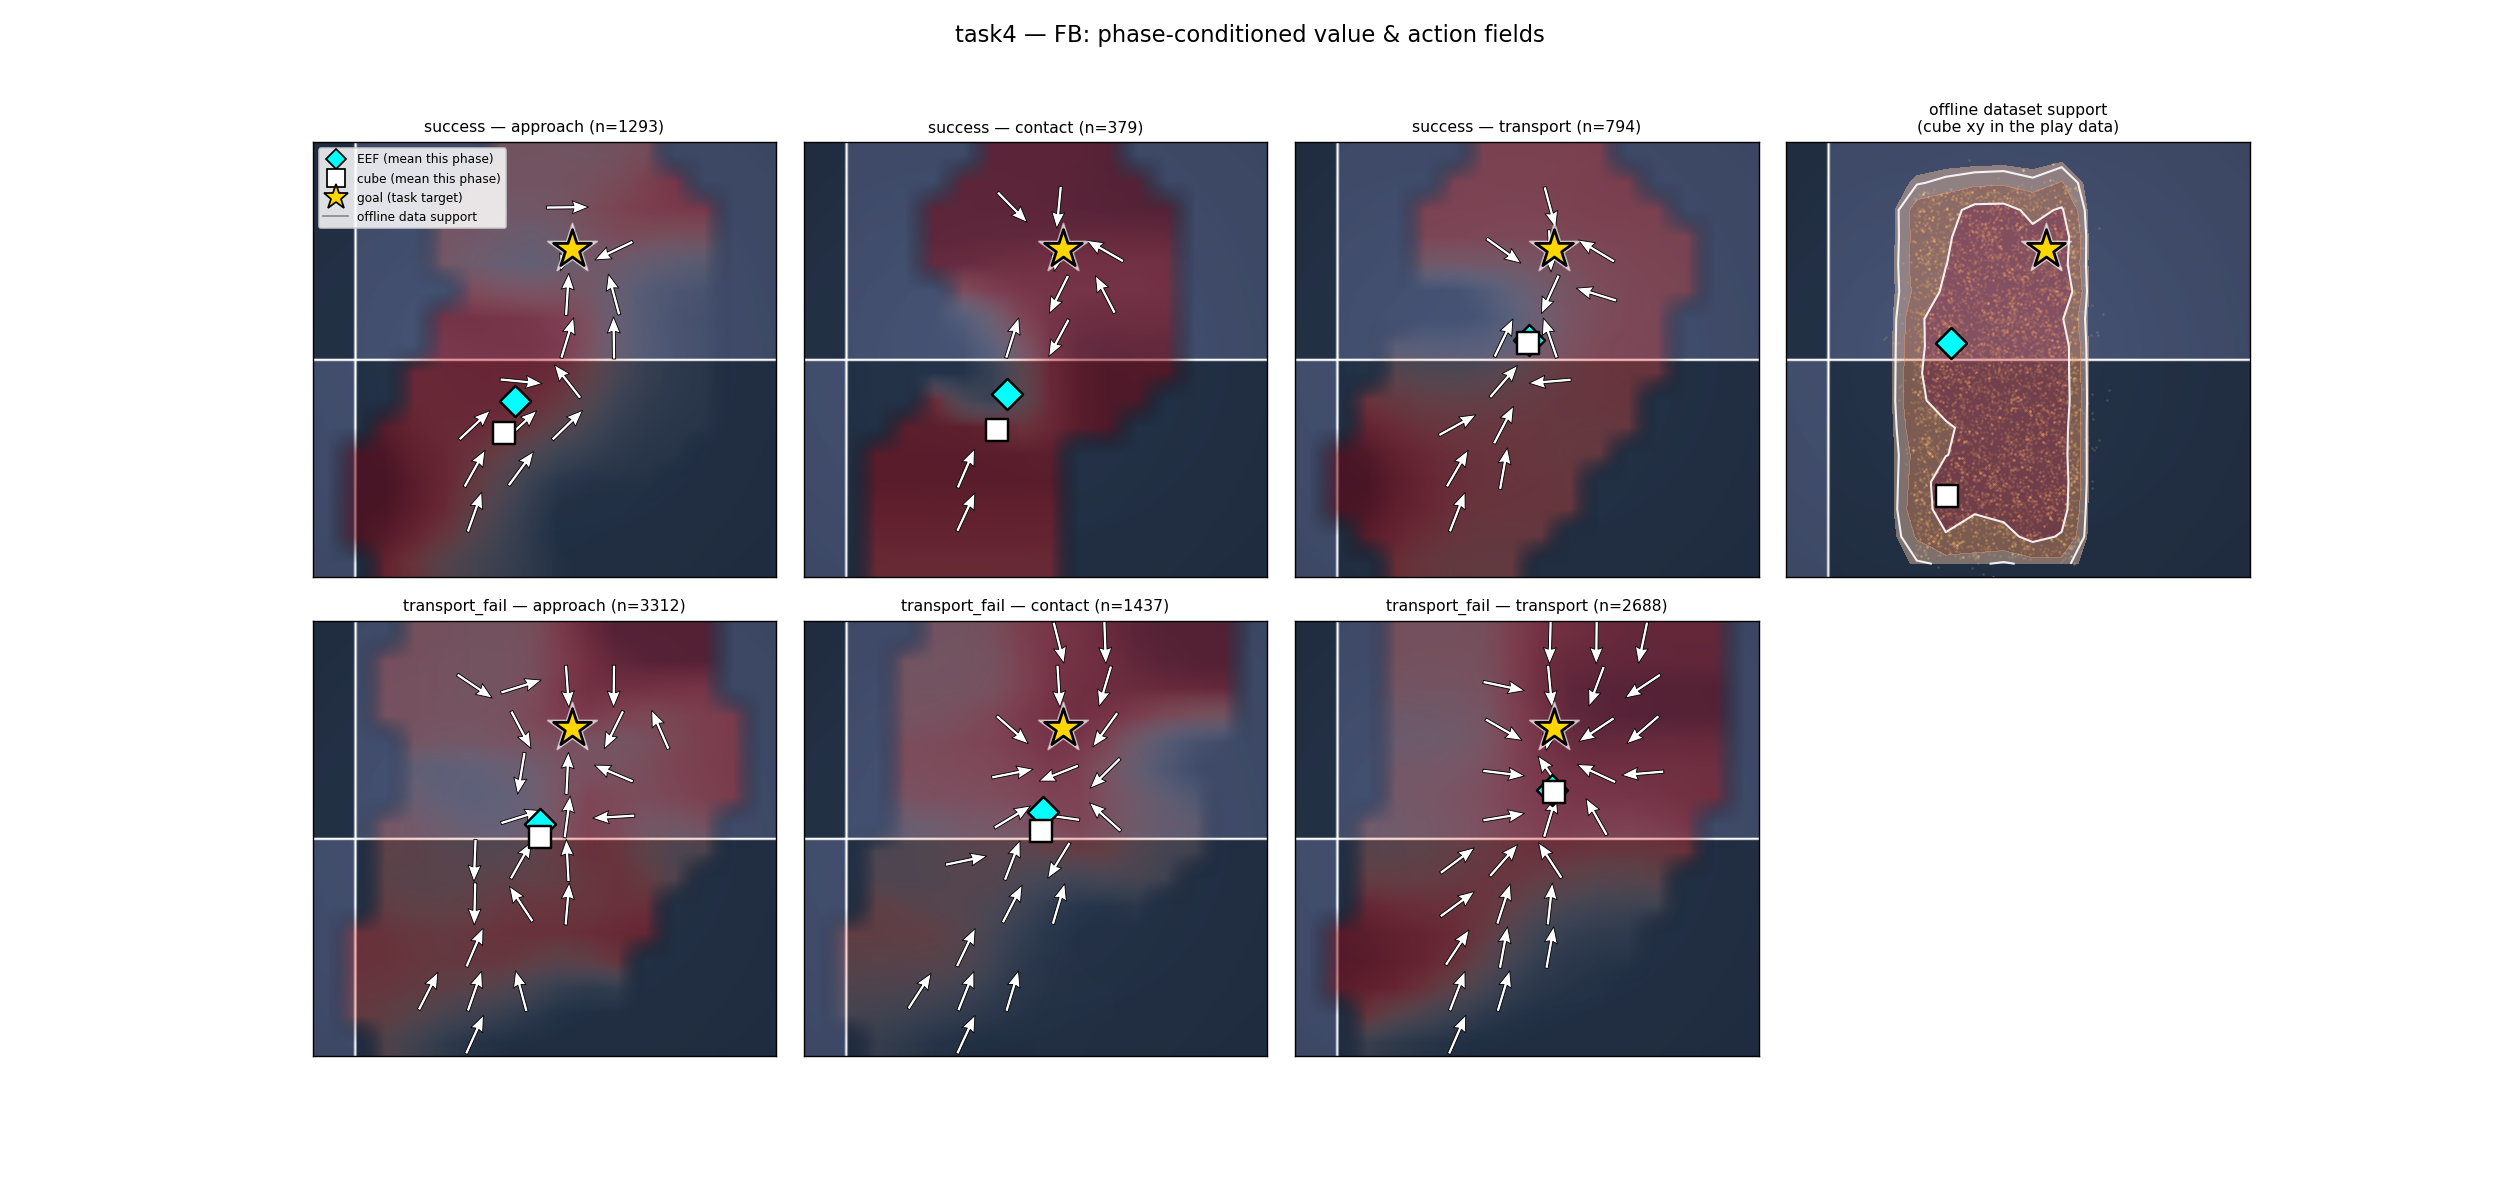
\includegraphics[width=\linewidth]{figures/state/task4__FB.png}
        \caption{task4 -- FB.}
    \end{subfigure}\hfill
    \begin{subfigure}{0.49\linewidth}
        \centering
        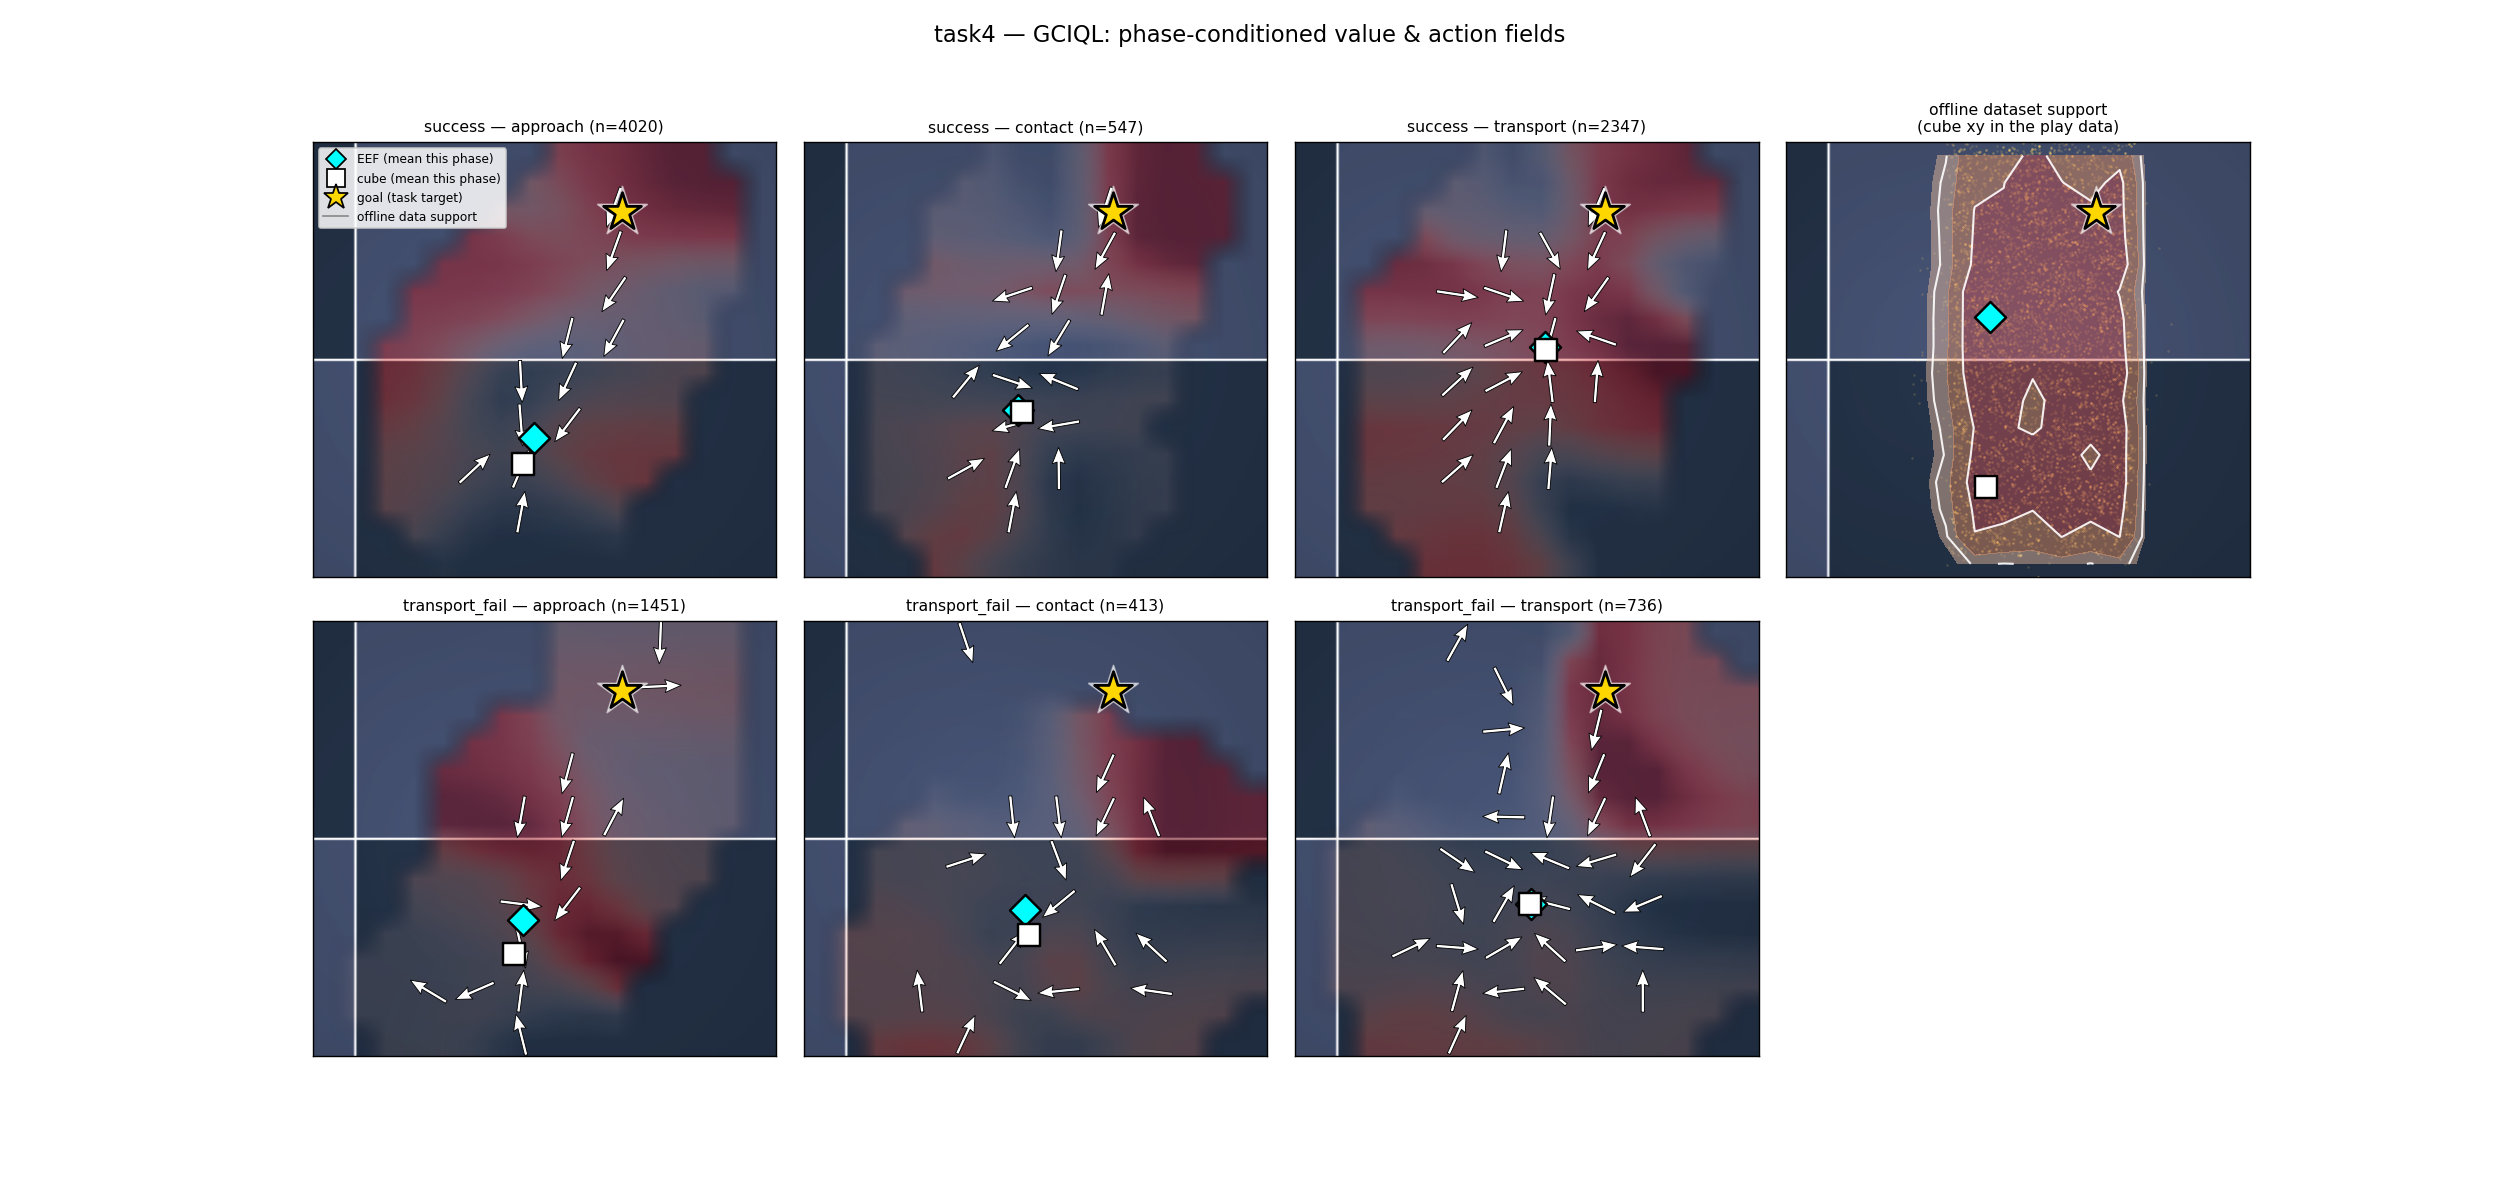
\includegraphics[width=\linewidth]{figures/state/task4__GCIQL.png}
        \caption{task4 -- GCIQL.}
    \end{subfigure}
    \caption{State observations: full phase-conditioned value/action fields for task4.}
\end{figure}

\begin{figure}[H]
    \centering
    \begin{subfigure}{0.49\linewidth}
        \centering
        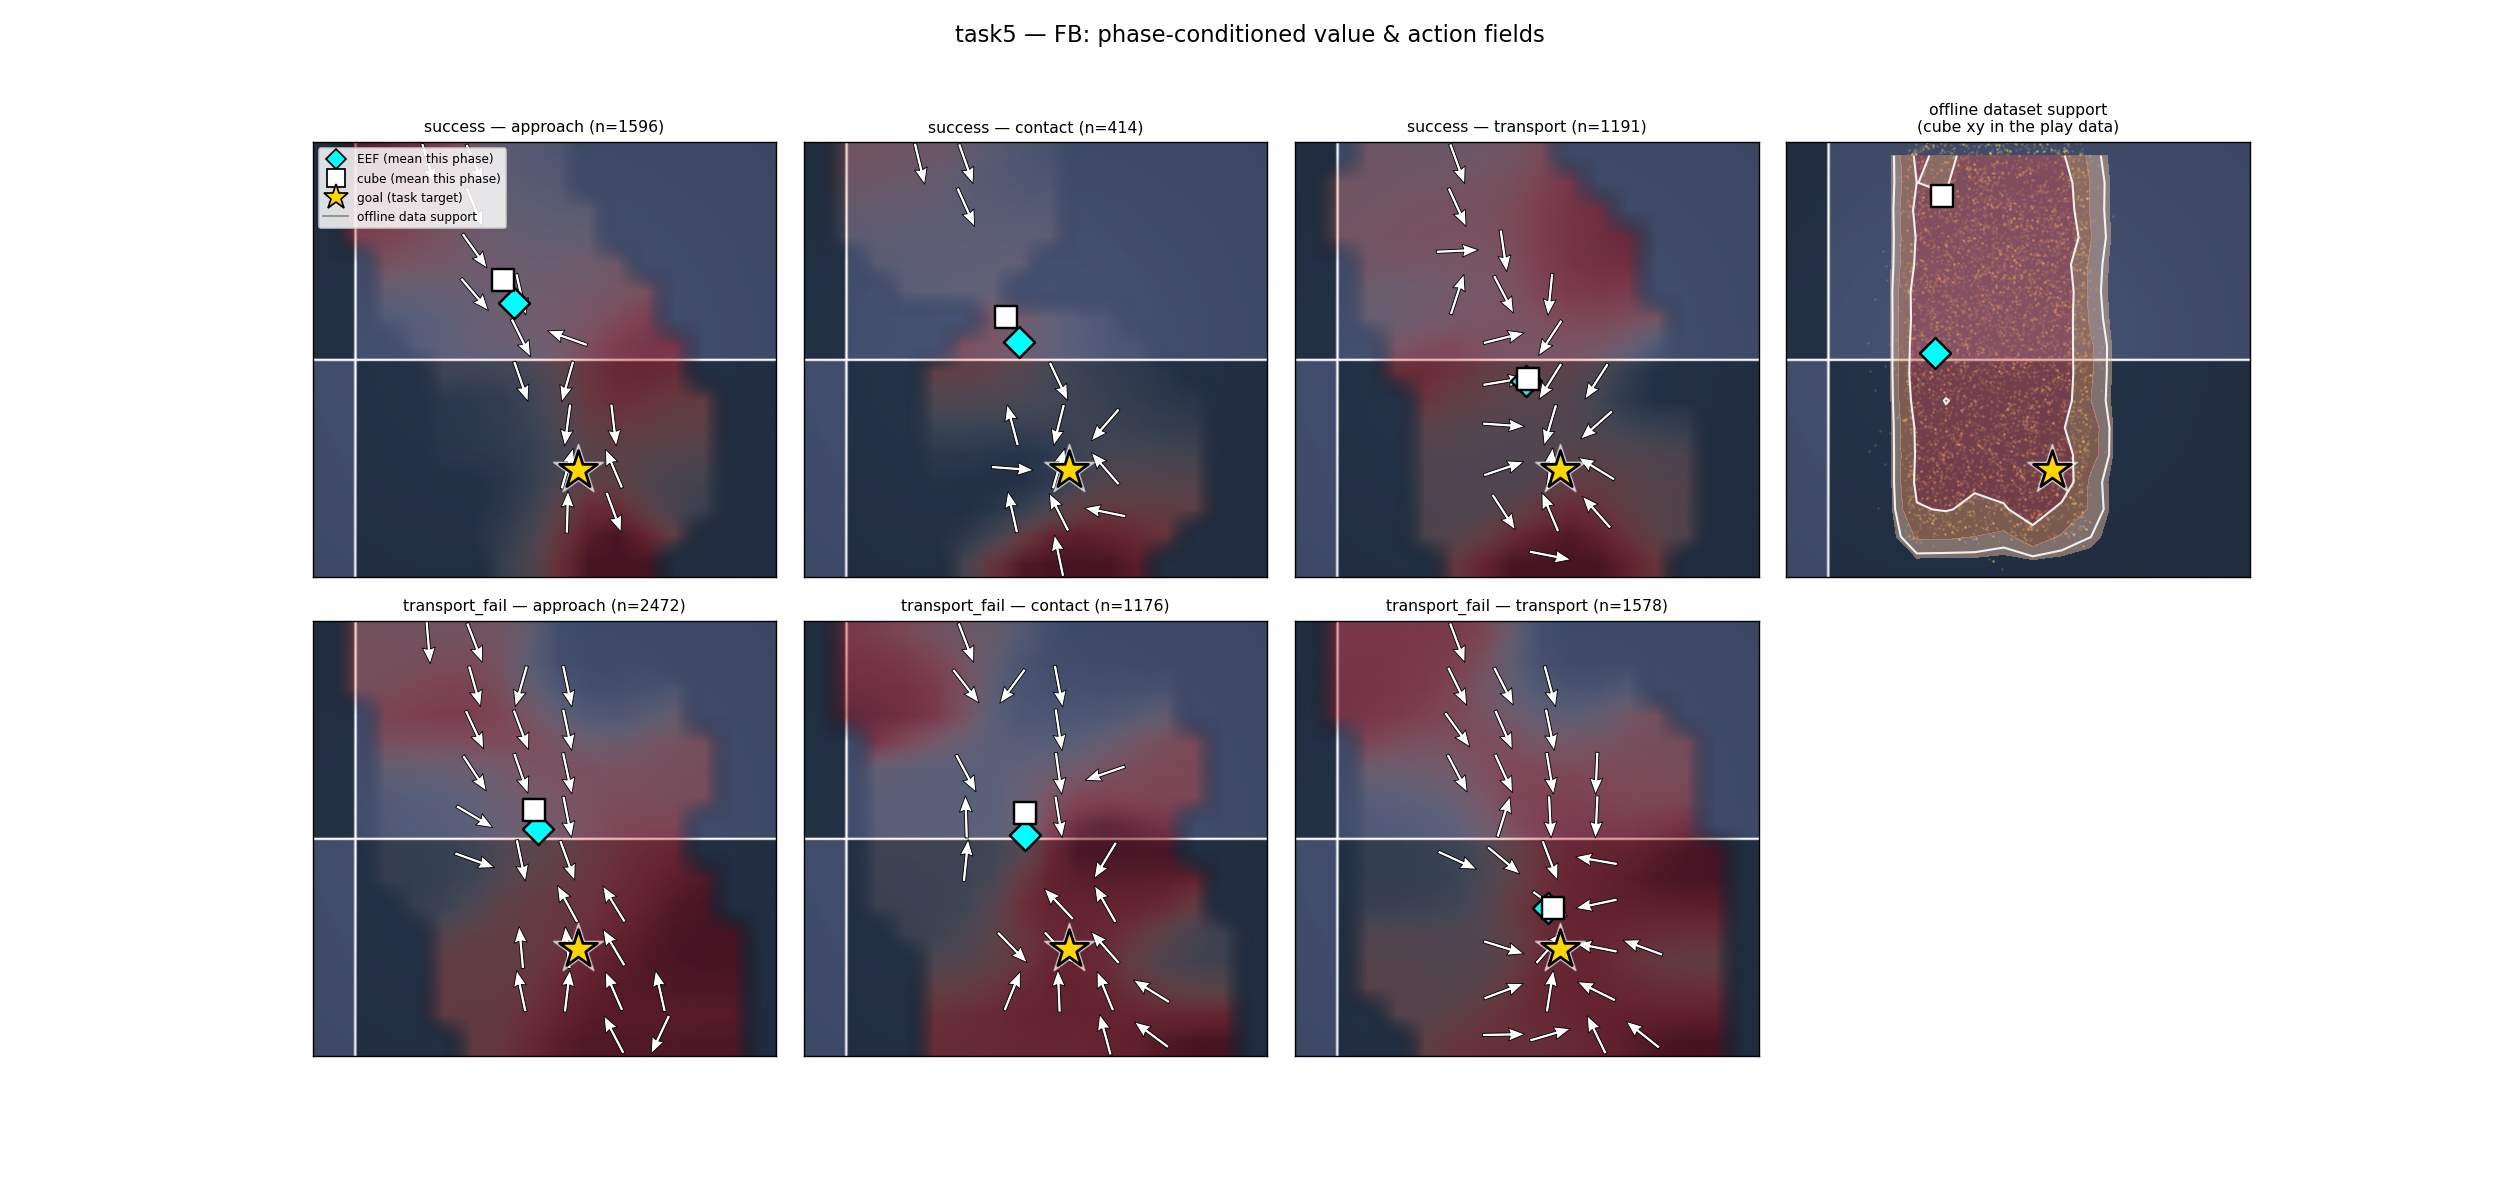
\includegraphics[width=\linewidth]{figures/state/task5__FB.png}
        \caption{task5 -- FB.}
    \end{subfigure}\hfill
    \begin{subfigure}{0.49\linewidth}
        \centering
        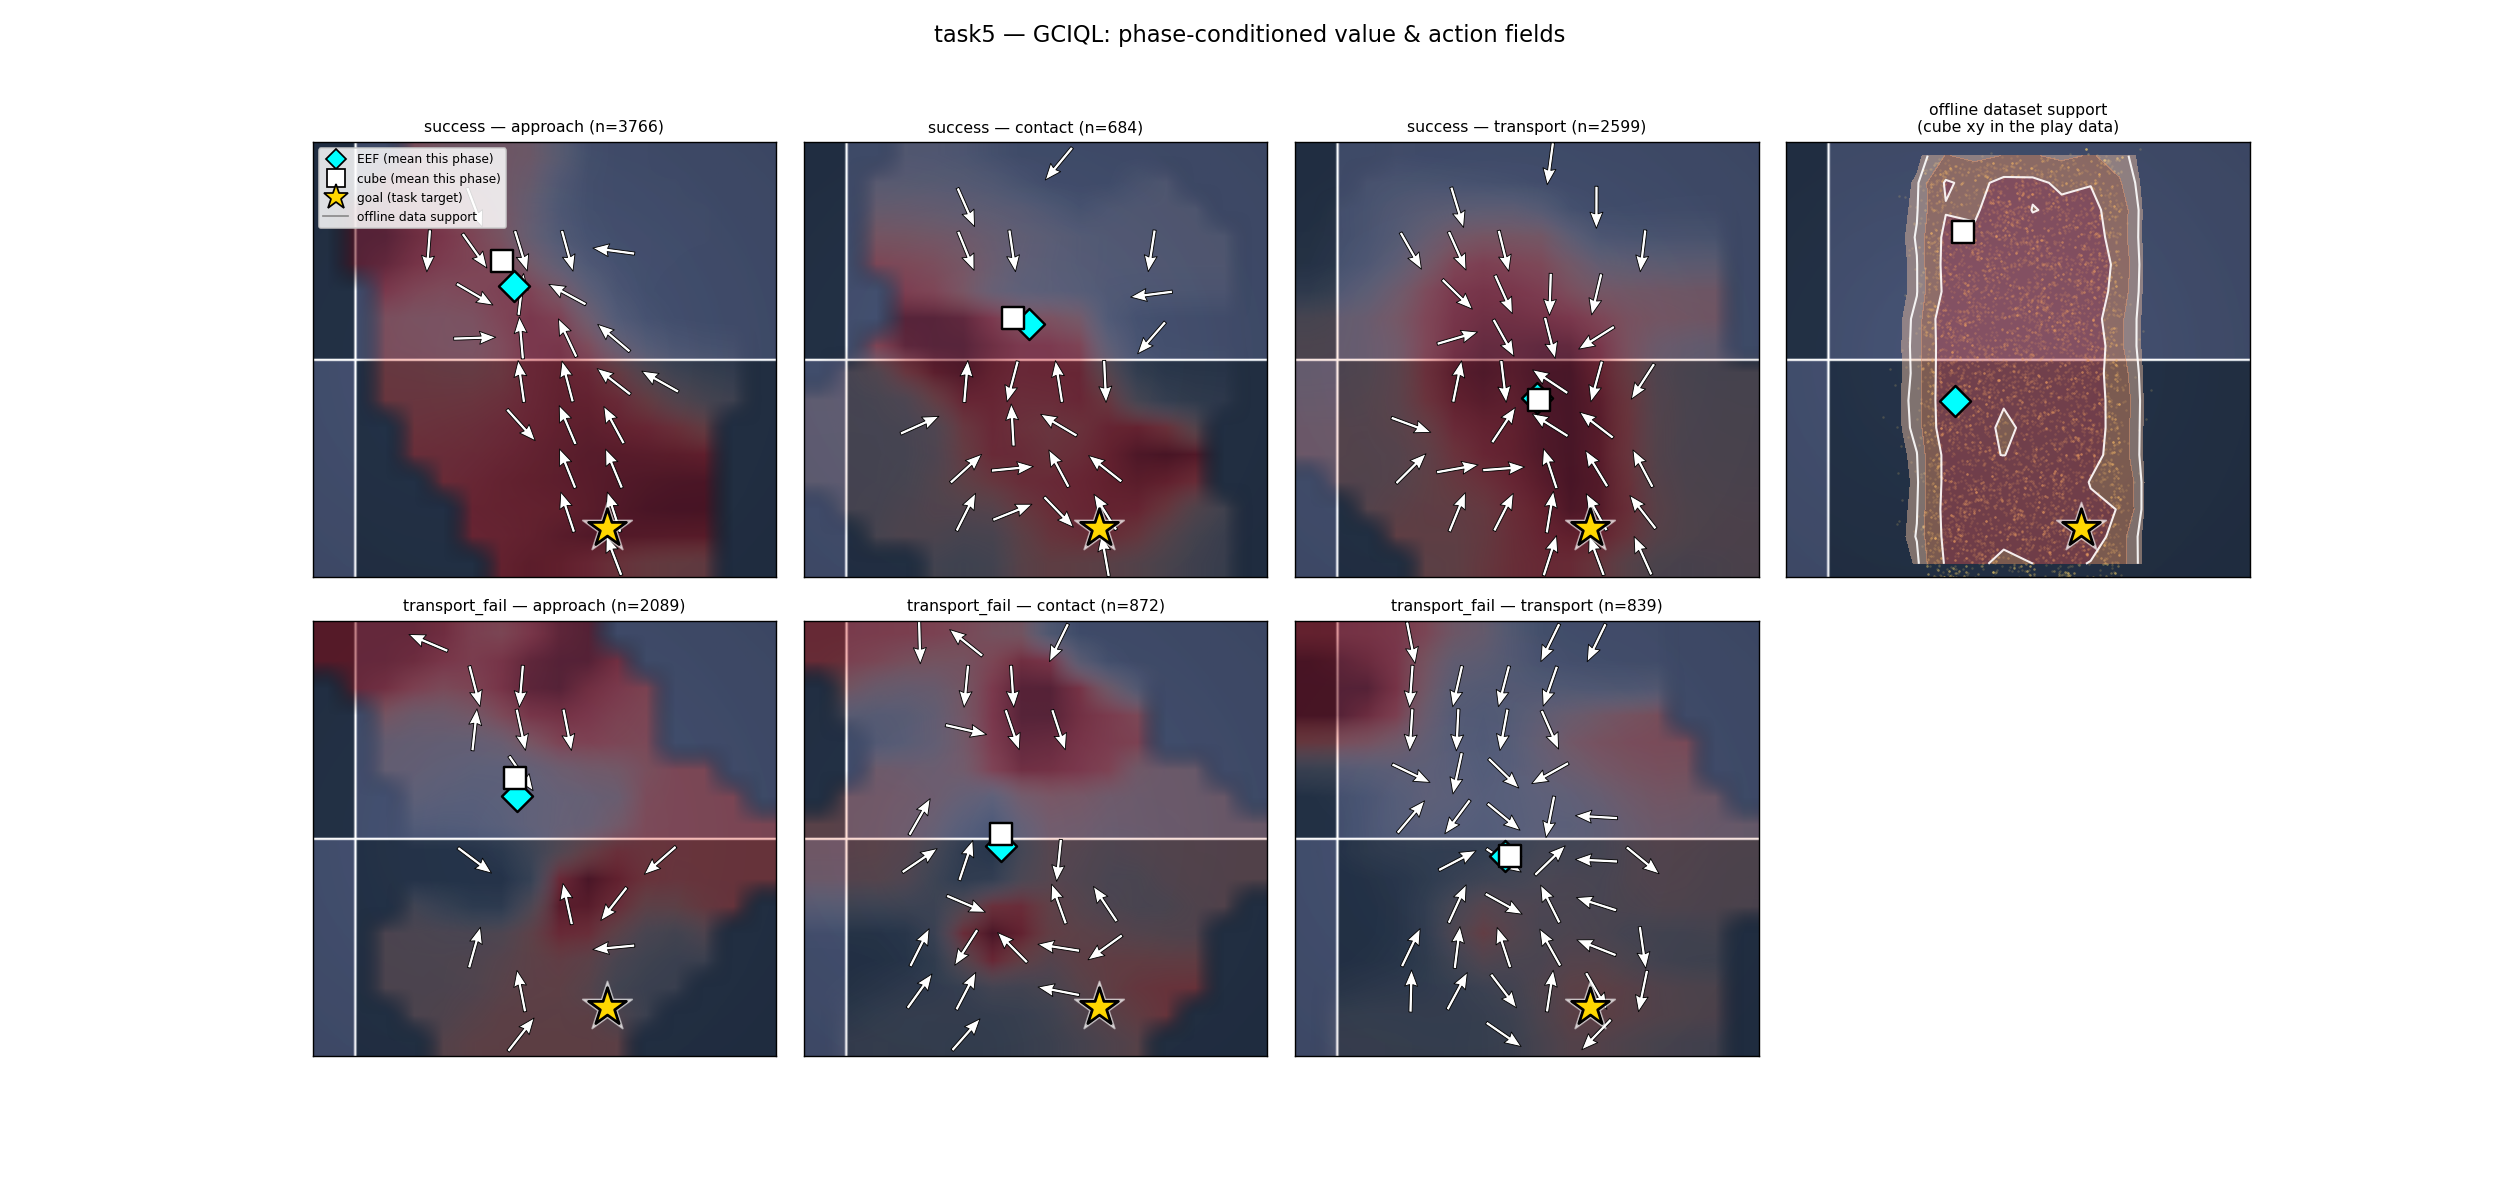
\includegraphics[width=\linewidth]{figures/state/task5__GCIQL.png}
        \caption{task5 -- GCIQL.}
    \end{subfigure}
    \caption{State observations: full phase-conditioned value/action fields for task5.}
\end{figure}

\section{Full Phase-Conditioned Value/Action Atlas: Pixel Observations}
\label{app:pixel-phase-atlas}

The following figures show the pixel-setting counterpart of \Cref{app:state-phase-atlas}.

\begin{figure}[H]
    \centering
    \begin{subfigure}{0.49\linewidth}
        \centering
        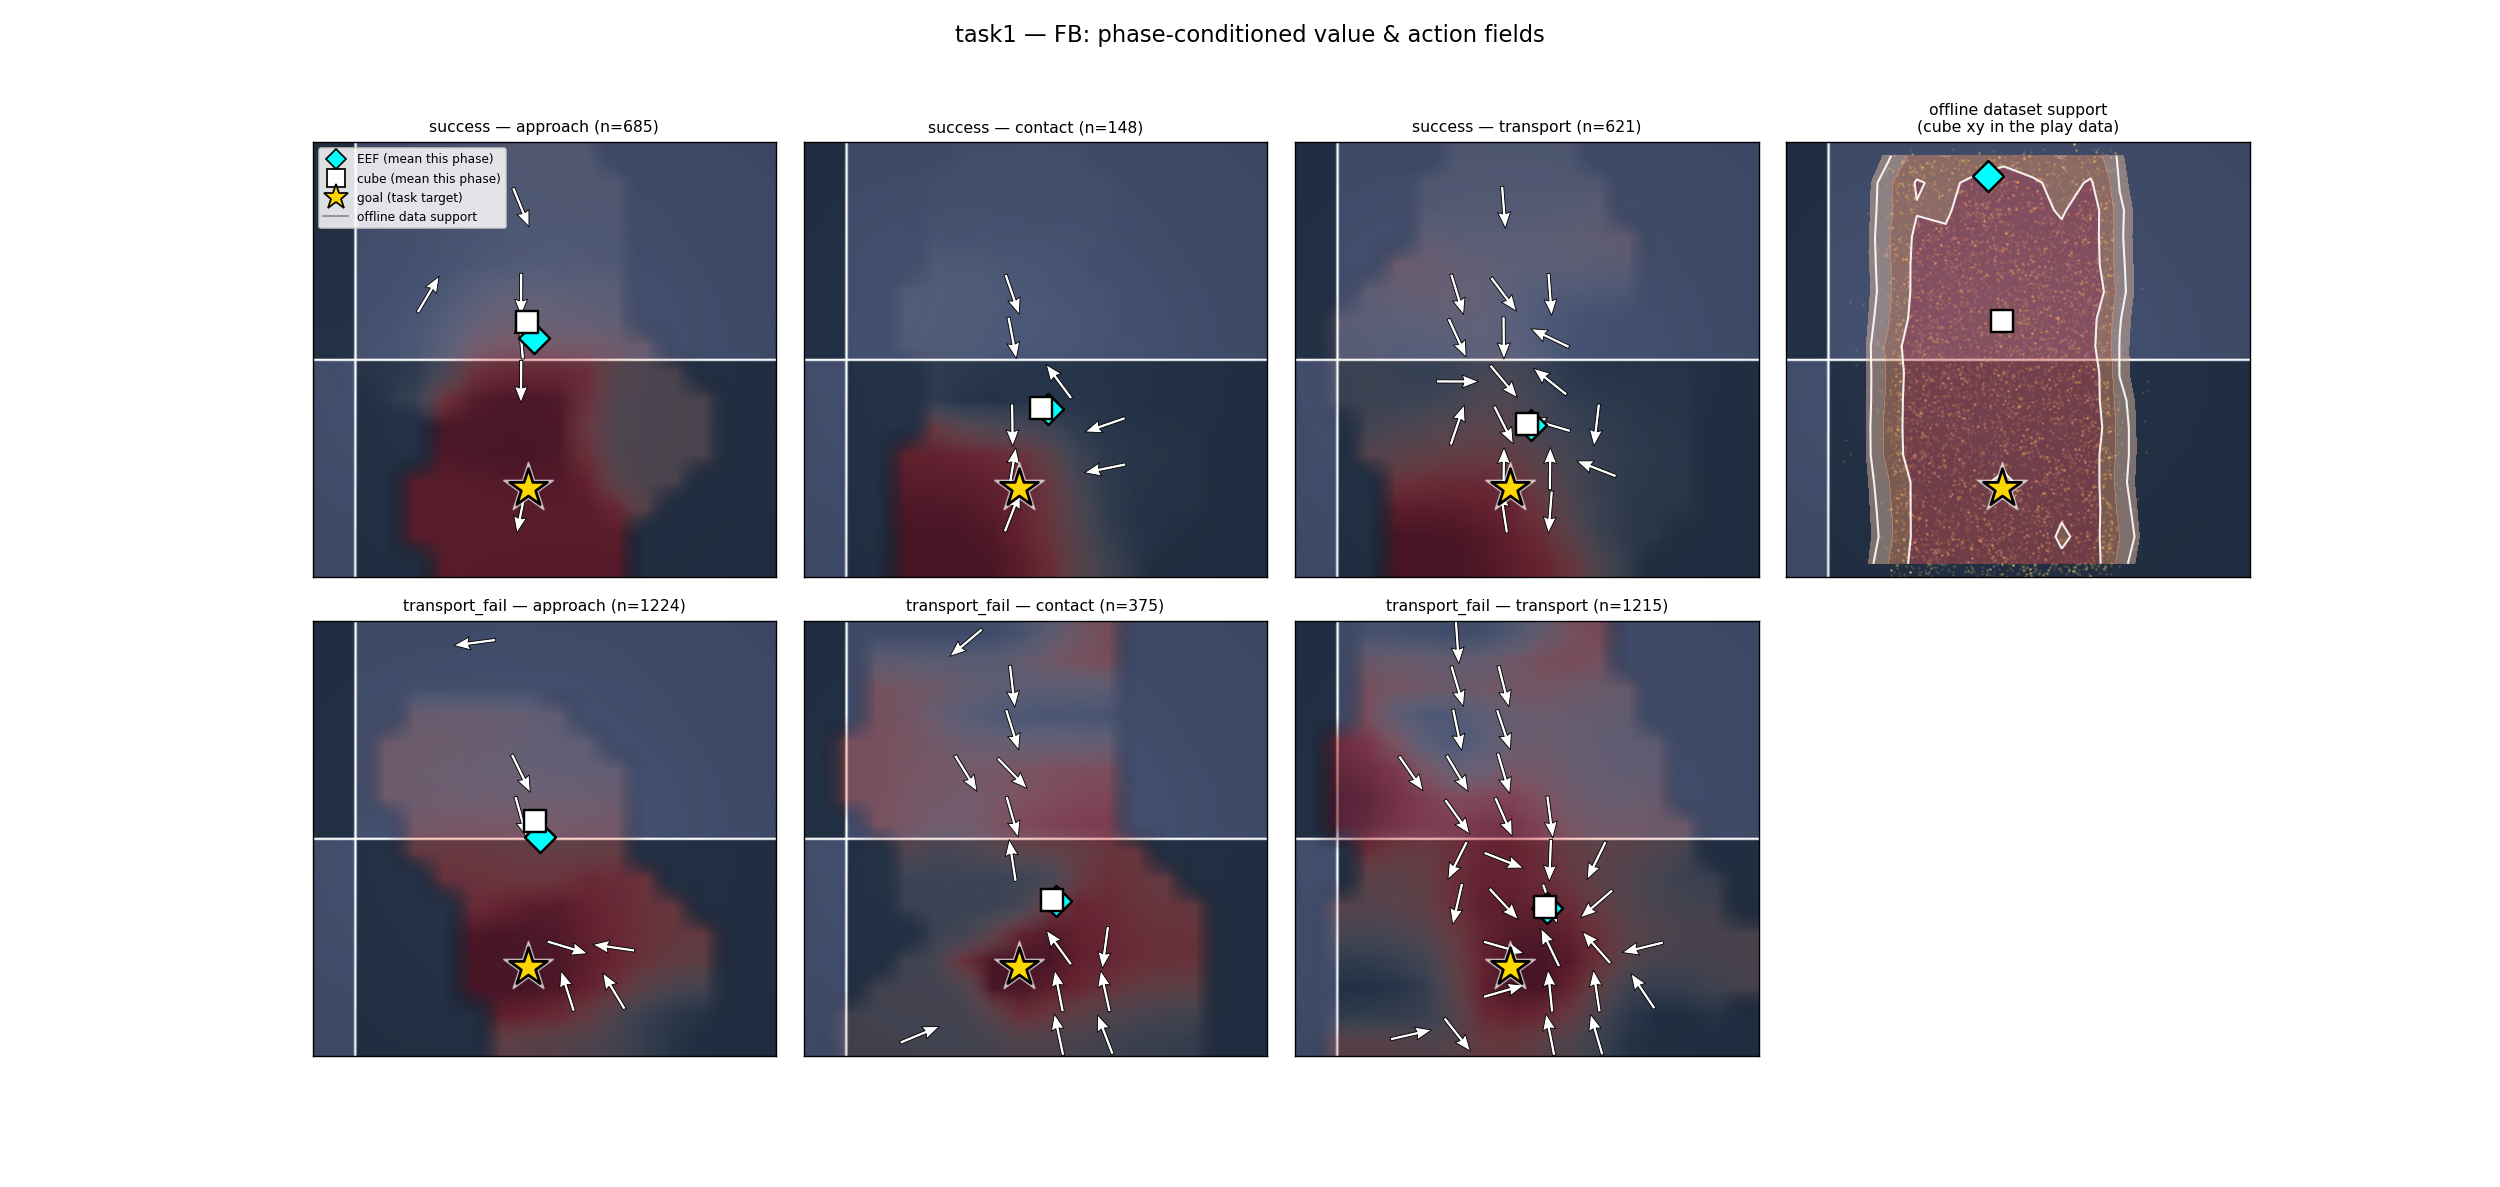
\includegraphics[width=\linewidth]{figures/pixel/pixel_phase_task1__FB.png}
        \caption{task1 -- FB.}
    \end{subfigure}\hfill
    \begin{subfigure}{0.49\linewidth}
        \centering
        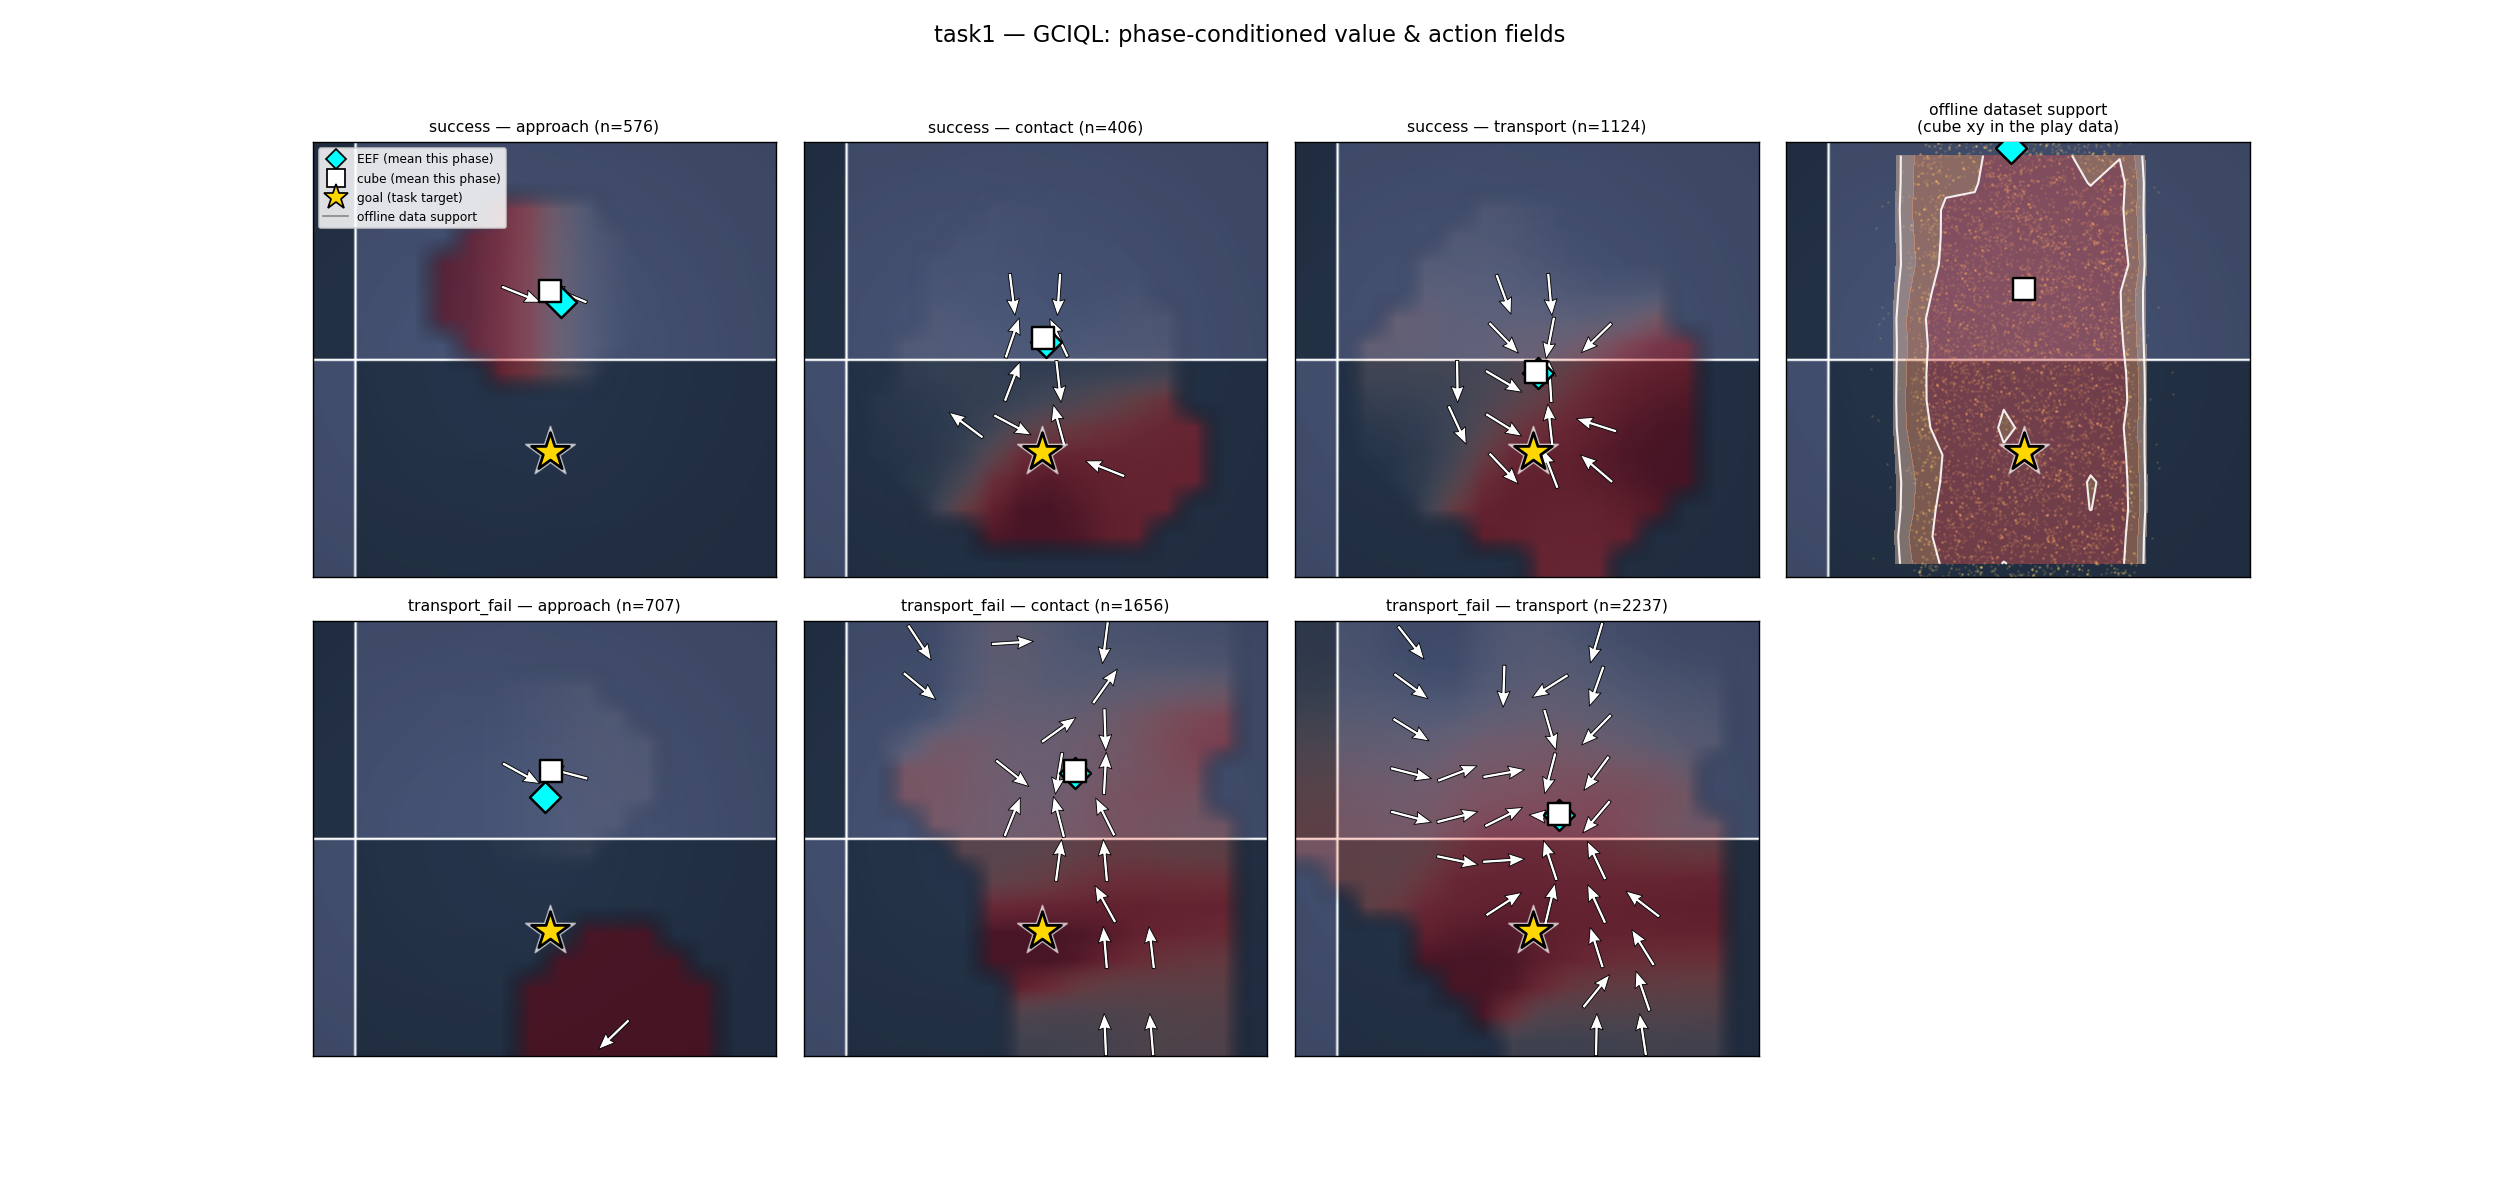
\includegraphics[width=\linewidth]{figures/pixel/pixel_phase_task1__GCIQL.png}
        \caption{task1 -- GCIQL.}
    \end{subfigure}
    \caption{Pixel observations: phase-conditioned value/action fields for task1.}
\end{figure}

\begin{figure}[H]
    \centering
    \begin{subfigure}{0.49\linewidth}
        \centering
        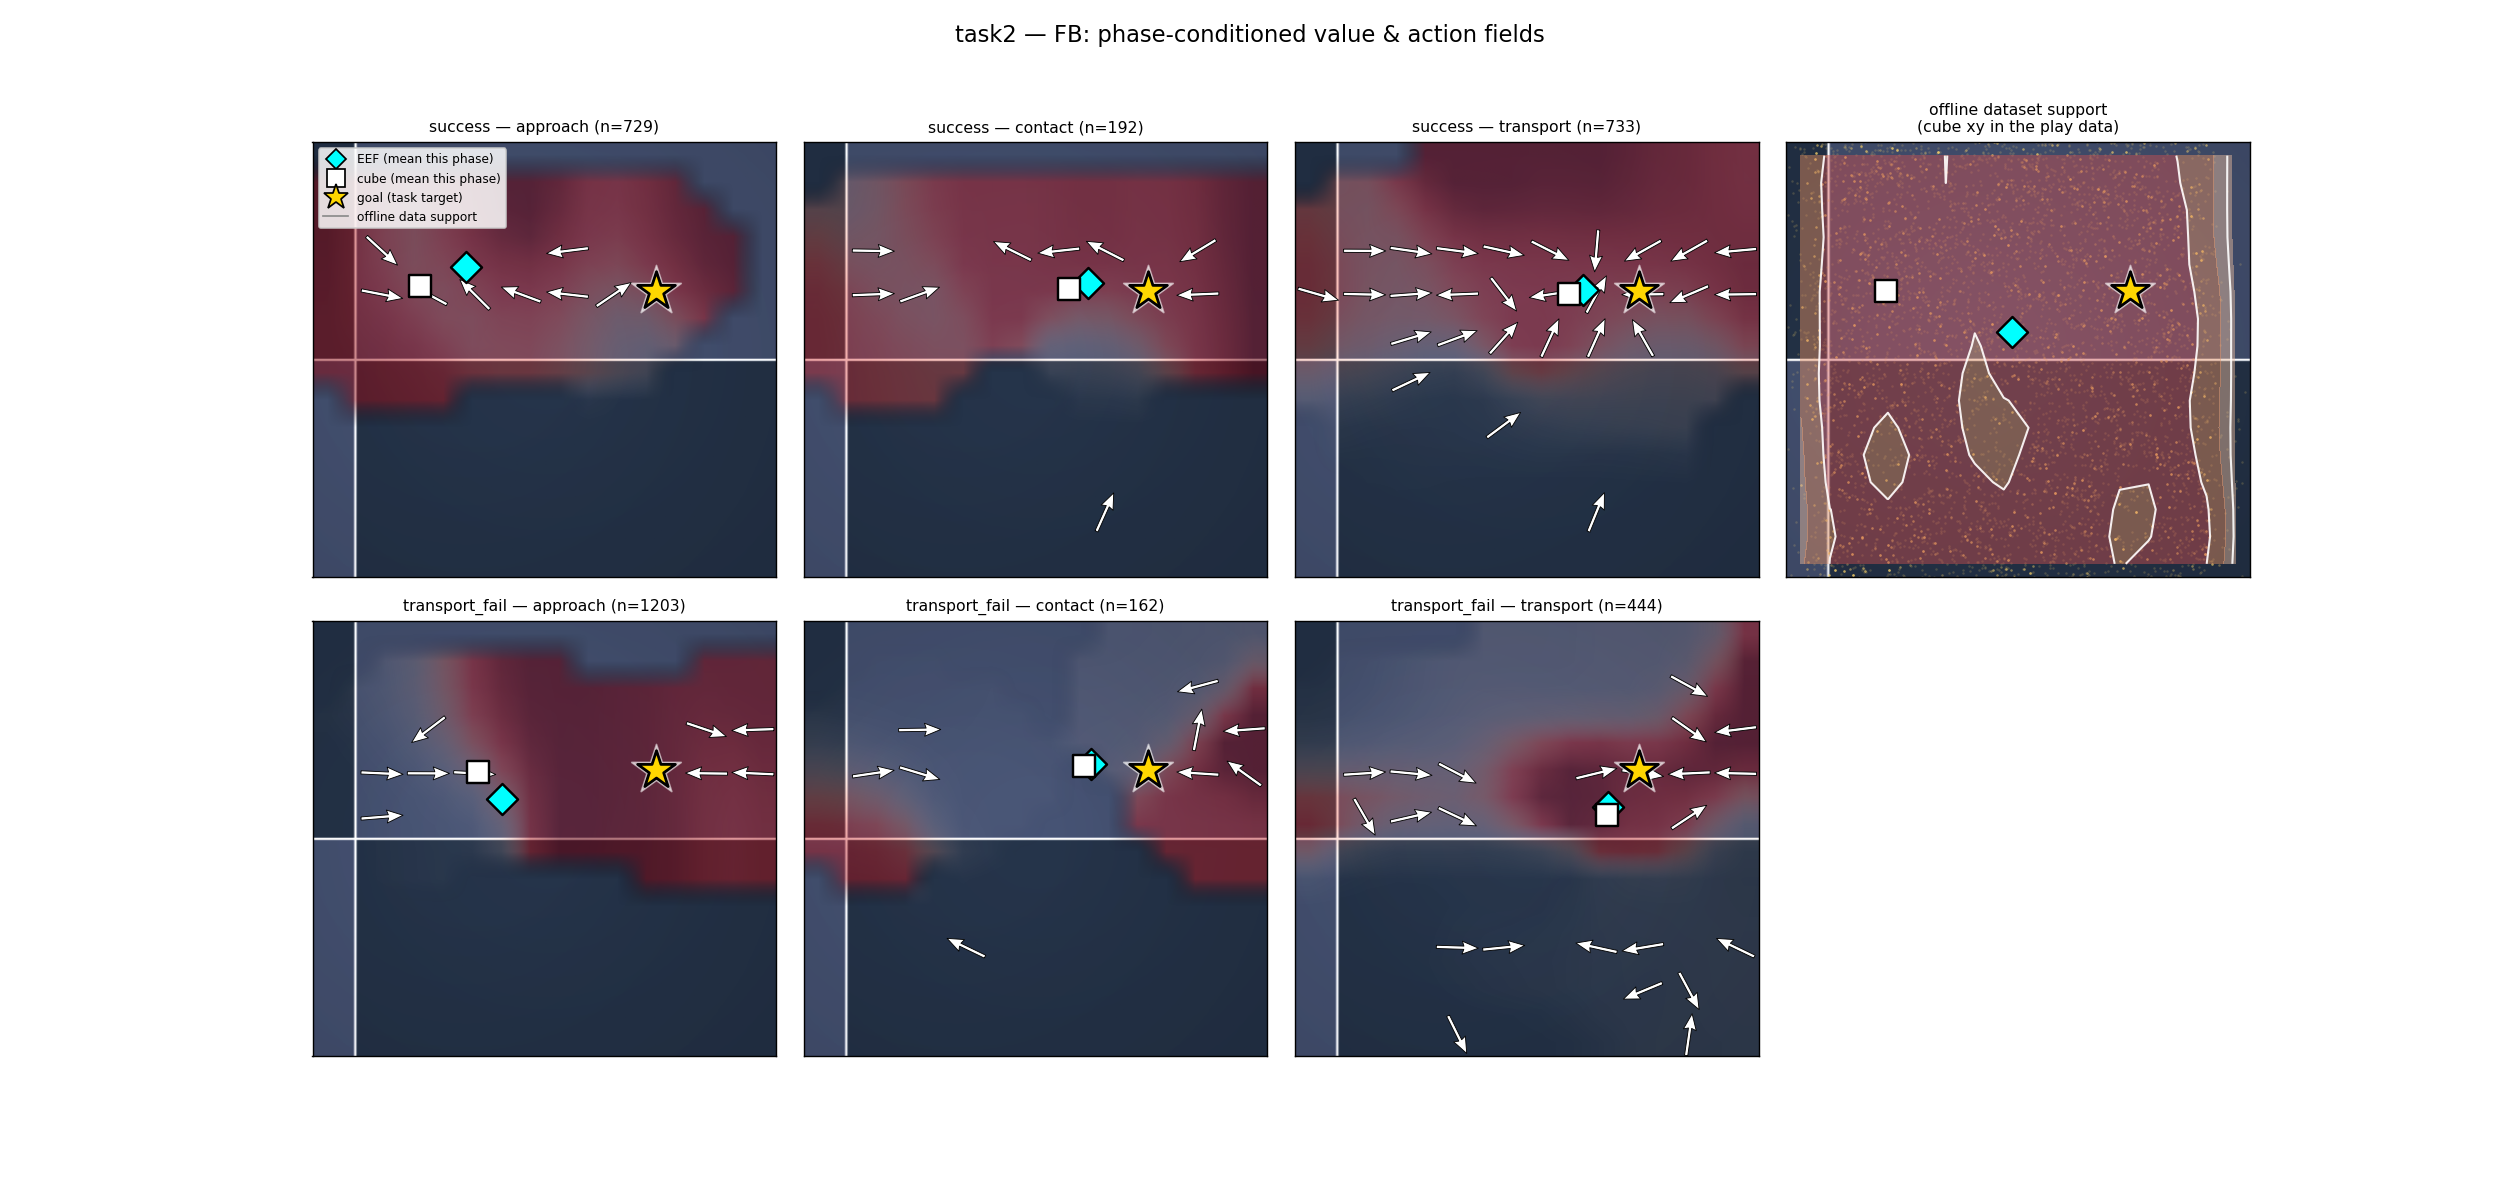
\includegraphics[width=\linewidth]{figures/pixel/pixel_phase_task2__FB.png}
        \caption{task2 -- FB.}
    \end{subfigure}\hfill
    \begin{subfigure}{0.49\linewidth}
        \centering
        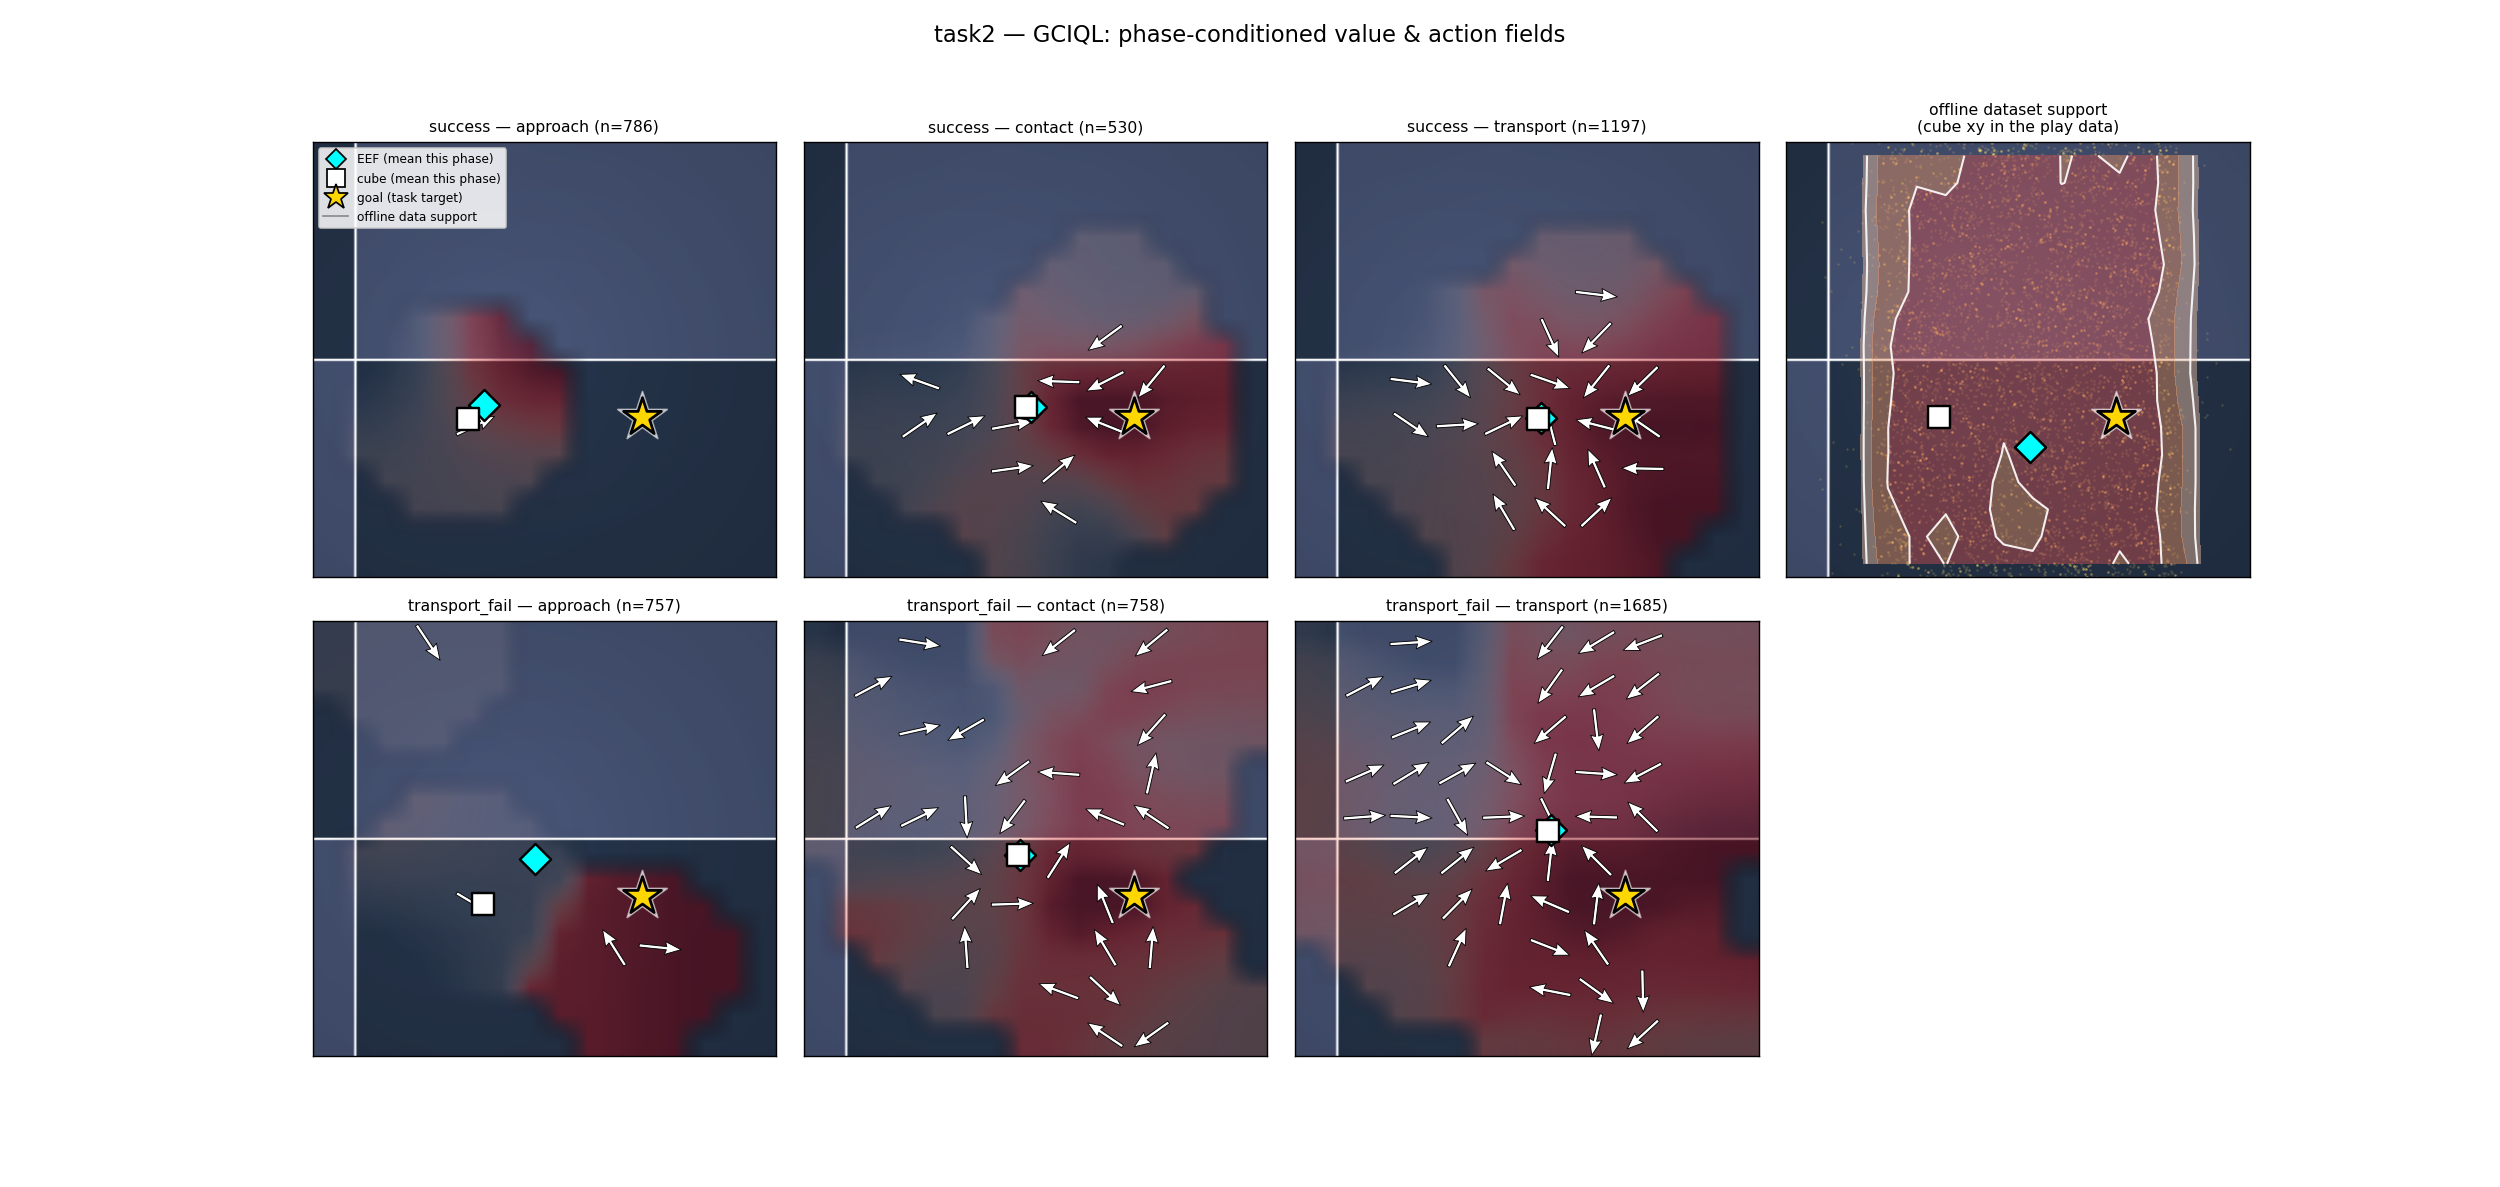
\includegraphics[width=\linewidth]{figures/pixel/pixel_phase_task2__GCIQL.png}
        \caption{task2 -- GCIQL.}
    \end{subfigure}
    \caption{Pixel observations: phase-conditioned value/action fields for task2.}
\end{figure}

\begin{figure}[H]
    \centering
    \begin{subfigure}{0.49\linewidth}
        \centering
        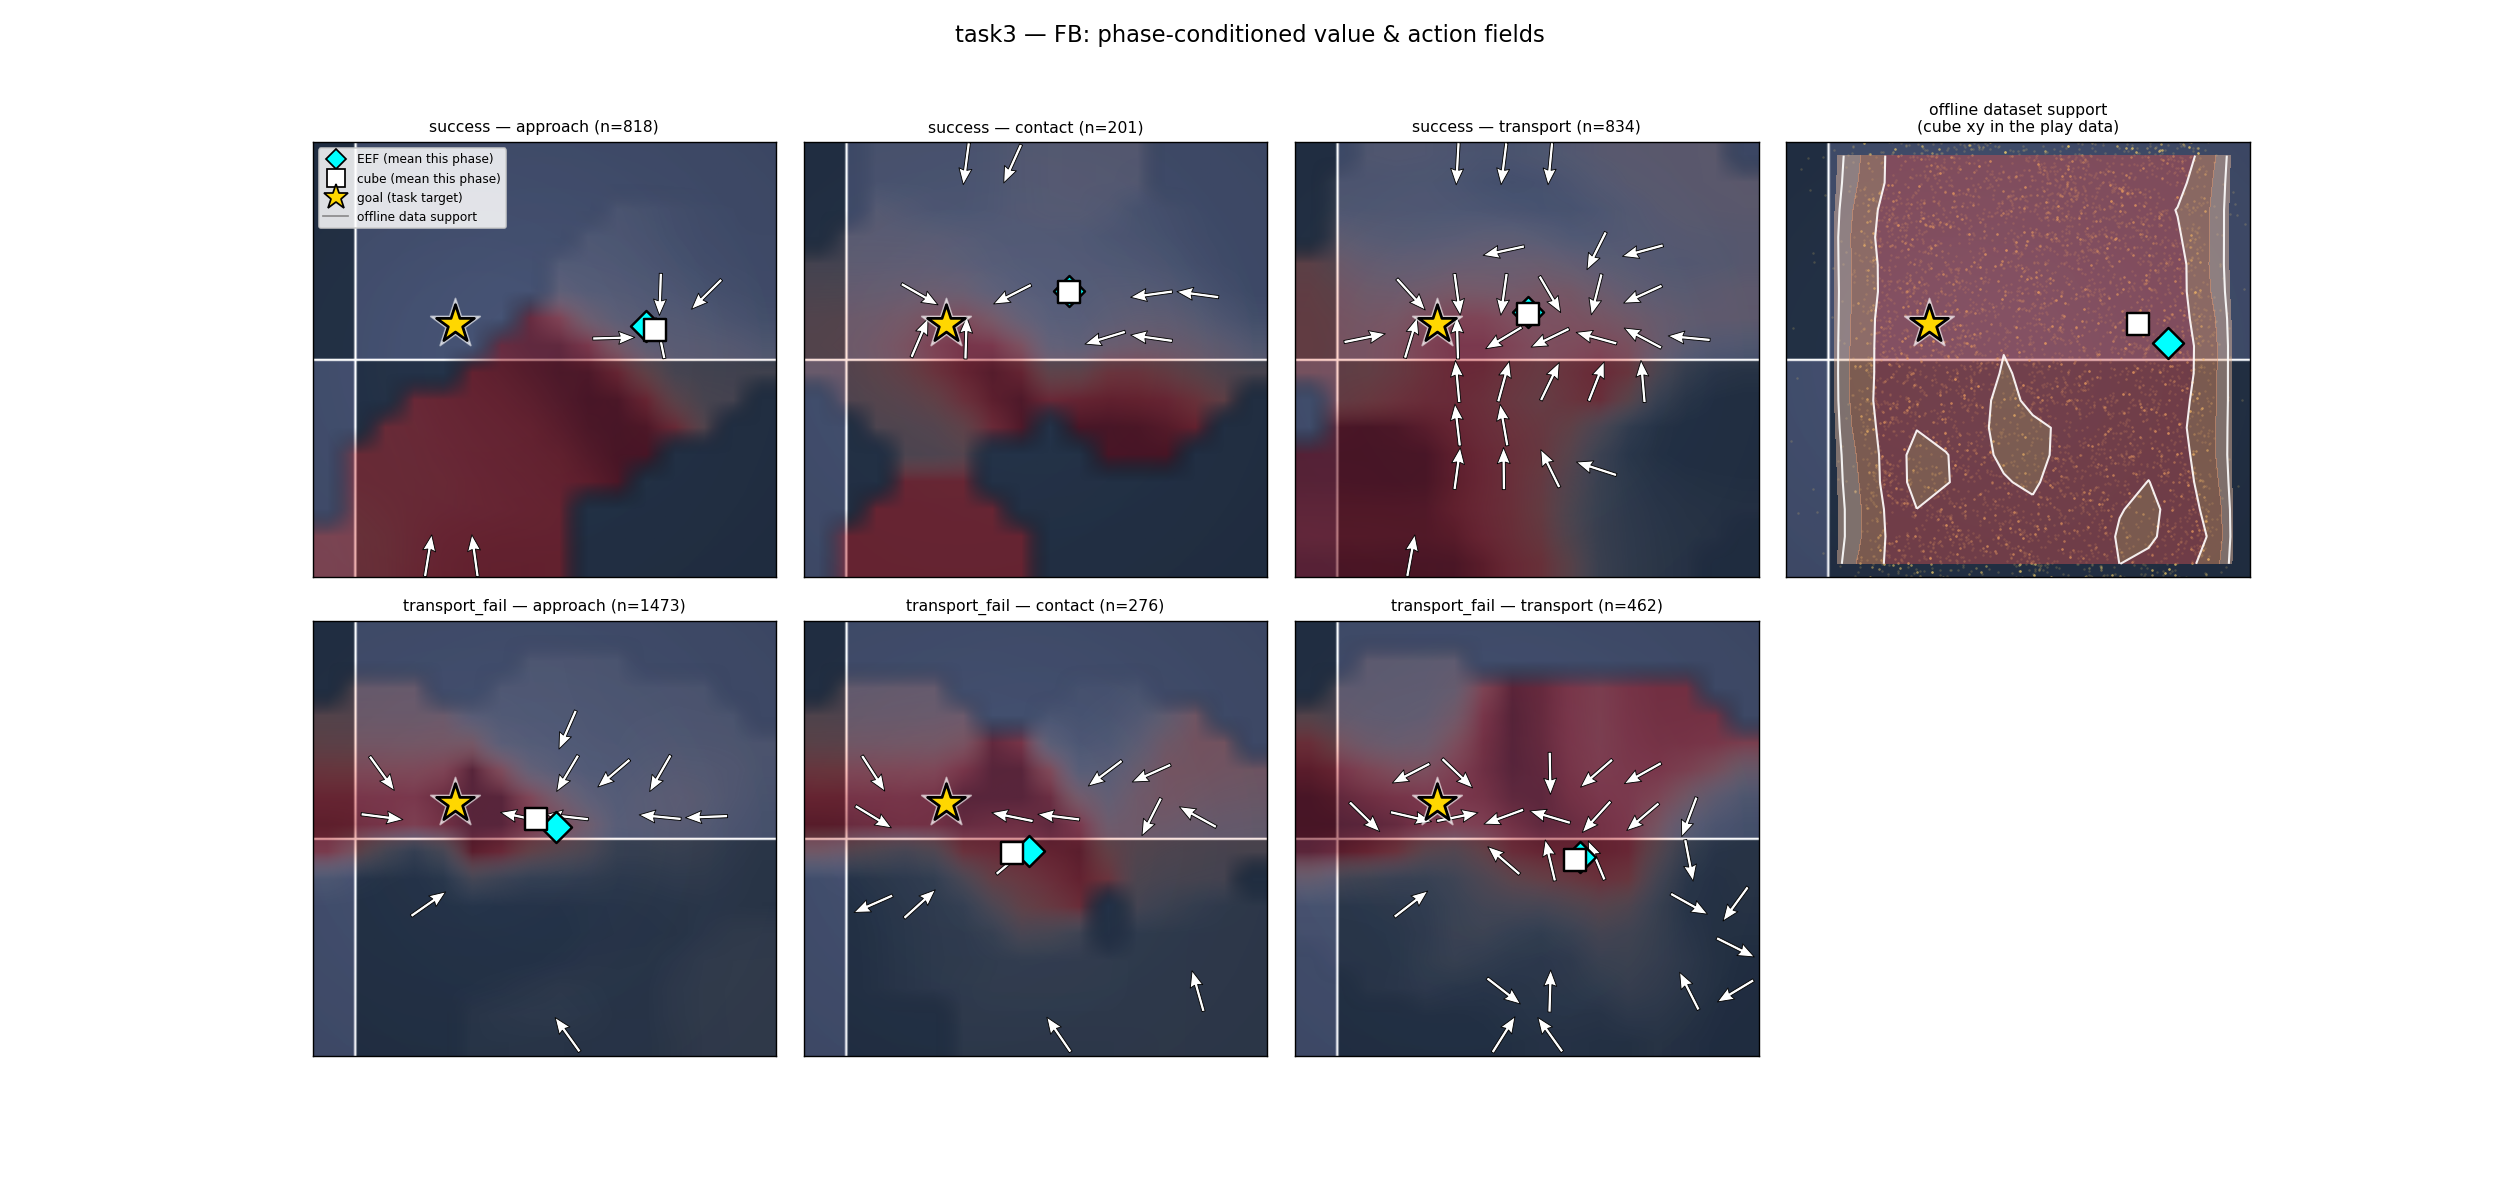
\includegraphics[width=\linewidth]{figures/pixel/pixel_phase_task3__FB.png}
        \caption{task3 -- FB.}
    \end{subfigure}\hfill
    \begin{subfigure}{0.49\linewidth}
        \centering
        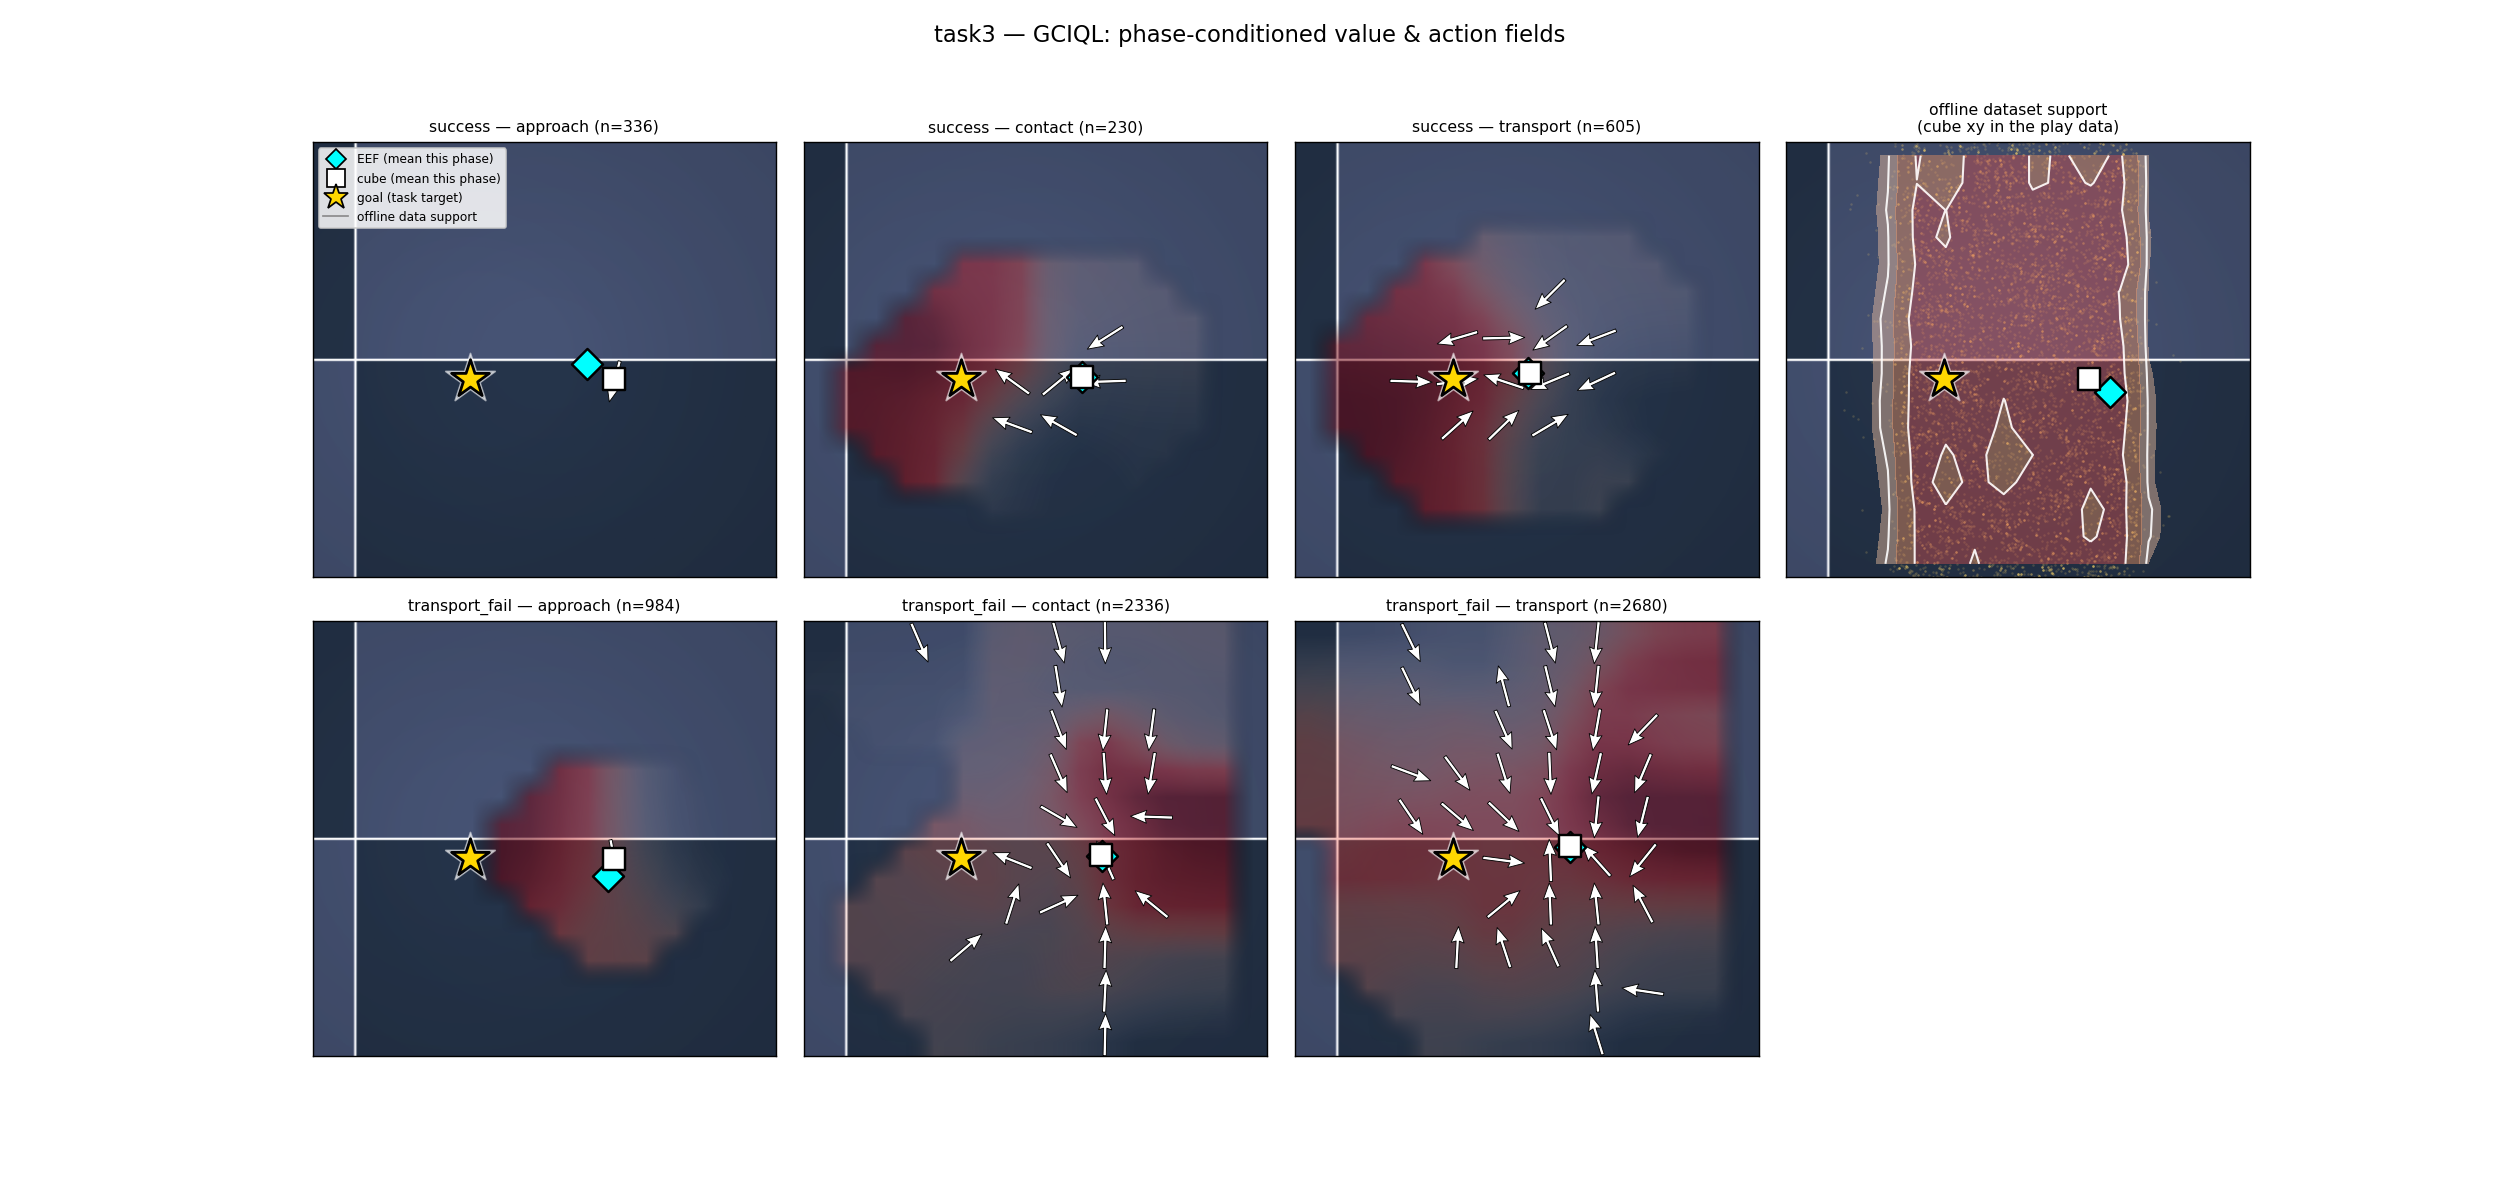
\includegraphics[width=\linewidth]{figures/pixel/pixel_phase_task3__GCIQL.png}
        \caption{task3 -- GCIQL.}
    \end{subfigure}
    \caption{Pixel observations: phase-conditioned value/action fields for task3.}
\end{figure}

\begin{figure}[H]
    \centering
    \begin{subfigure}{0.49\linewidth}
        \centering
        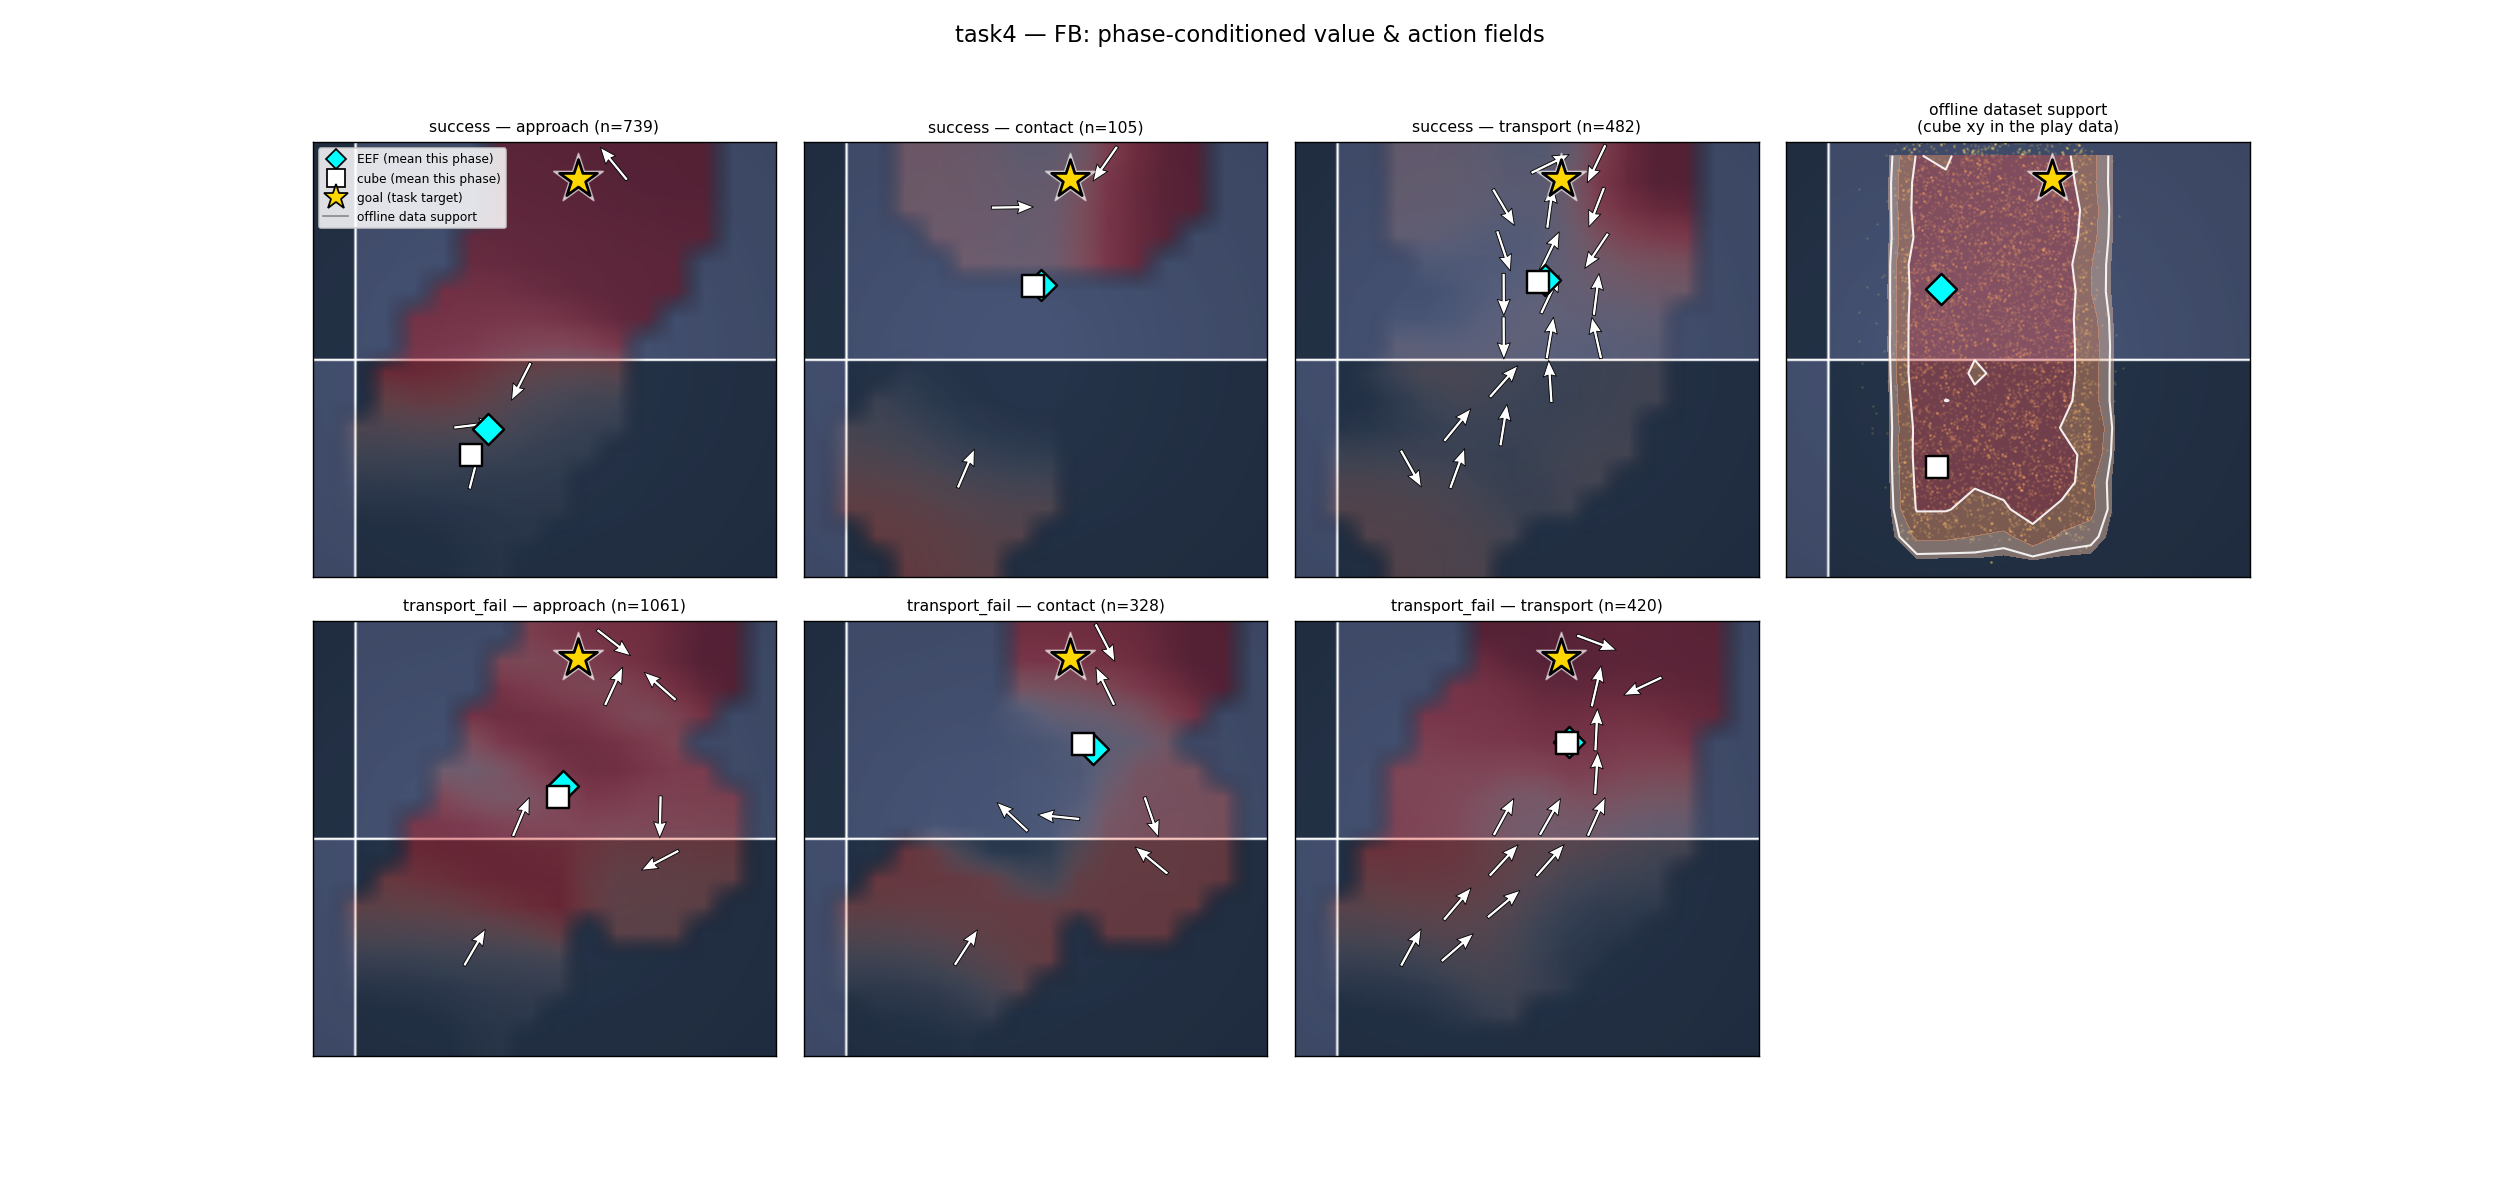
\includegraphics[width=\linewidth]{figures/pixel/pixel_phase_task4__FB.png}
        \caption{task4 -- FB.}
    \end{subfigure}\hfill
    \begin{subfigure}{0.49\linewidth}
        \centering
        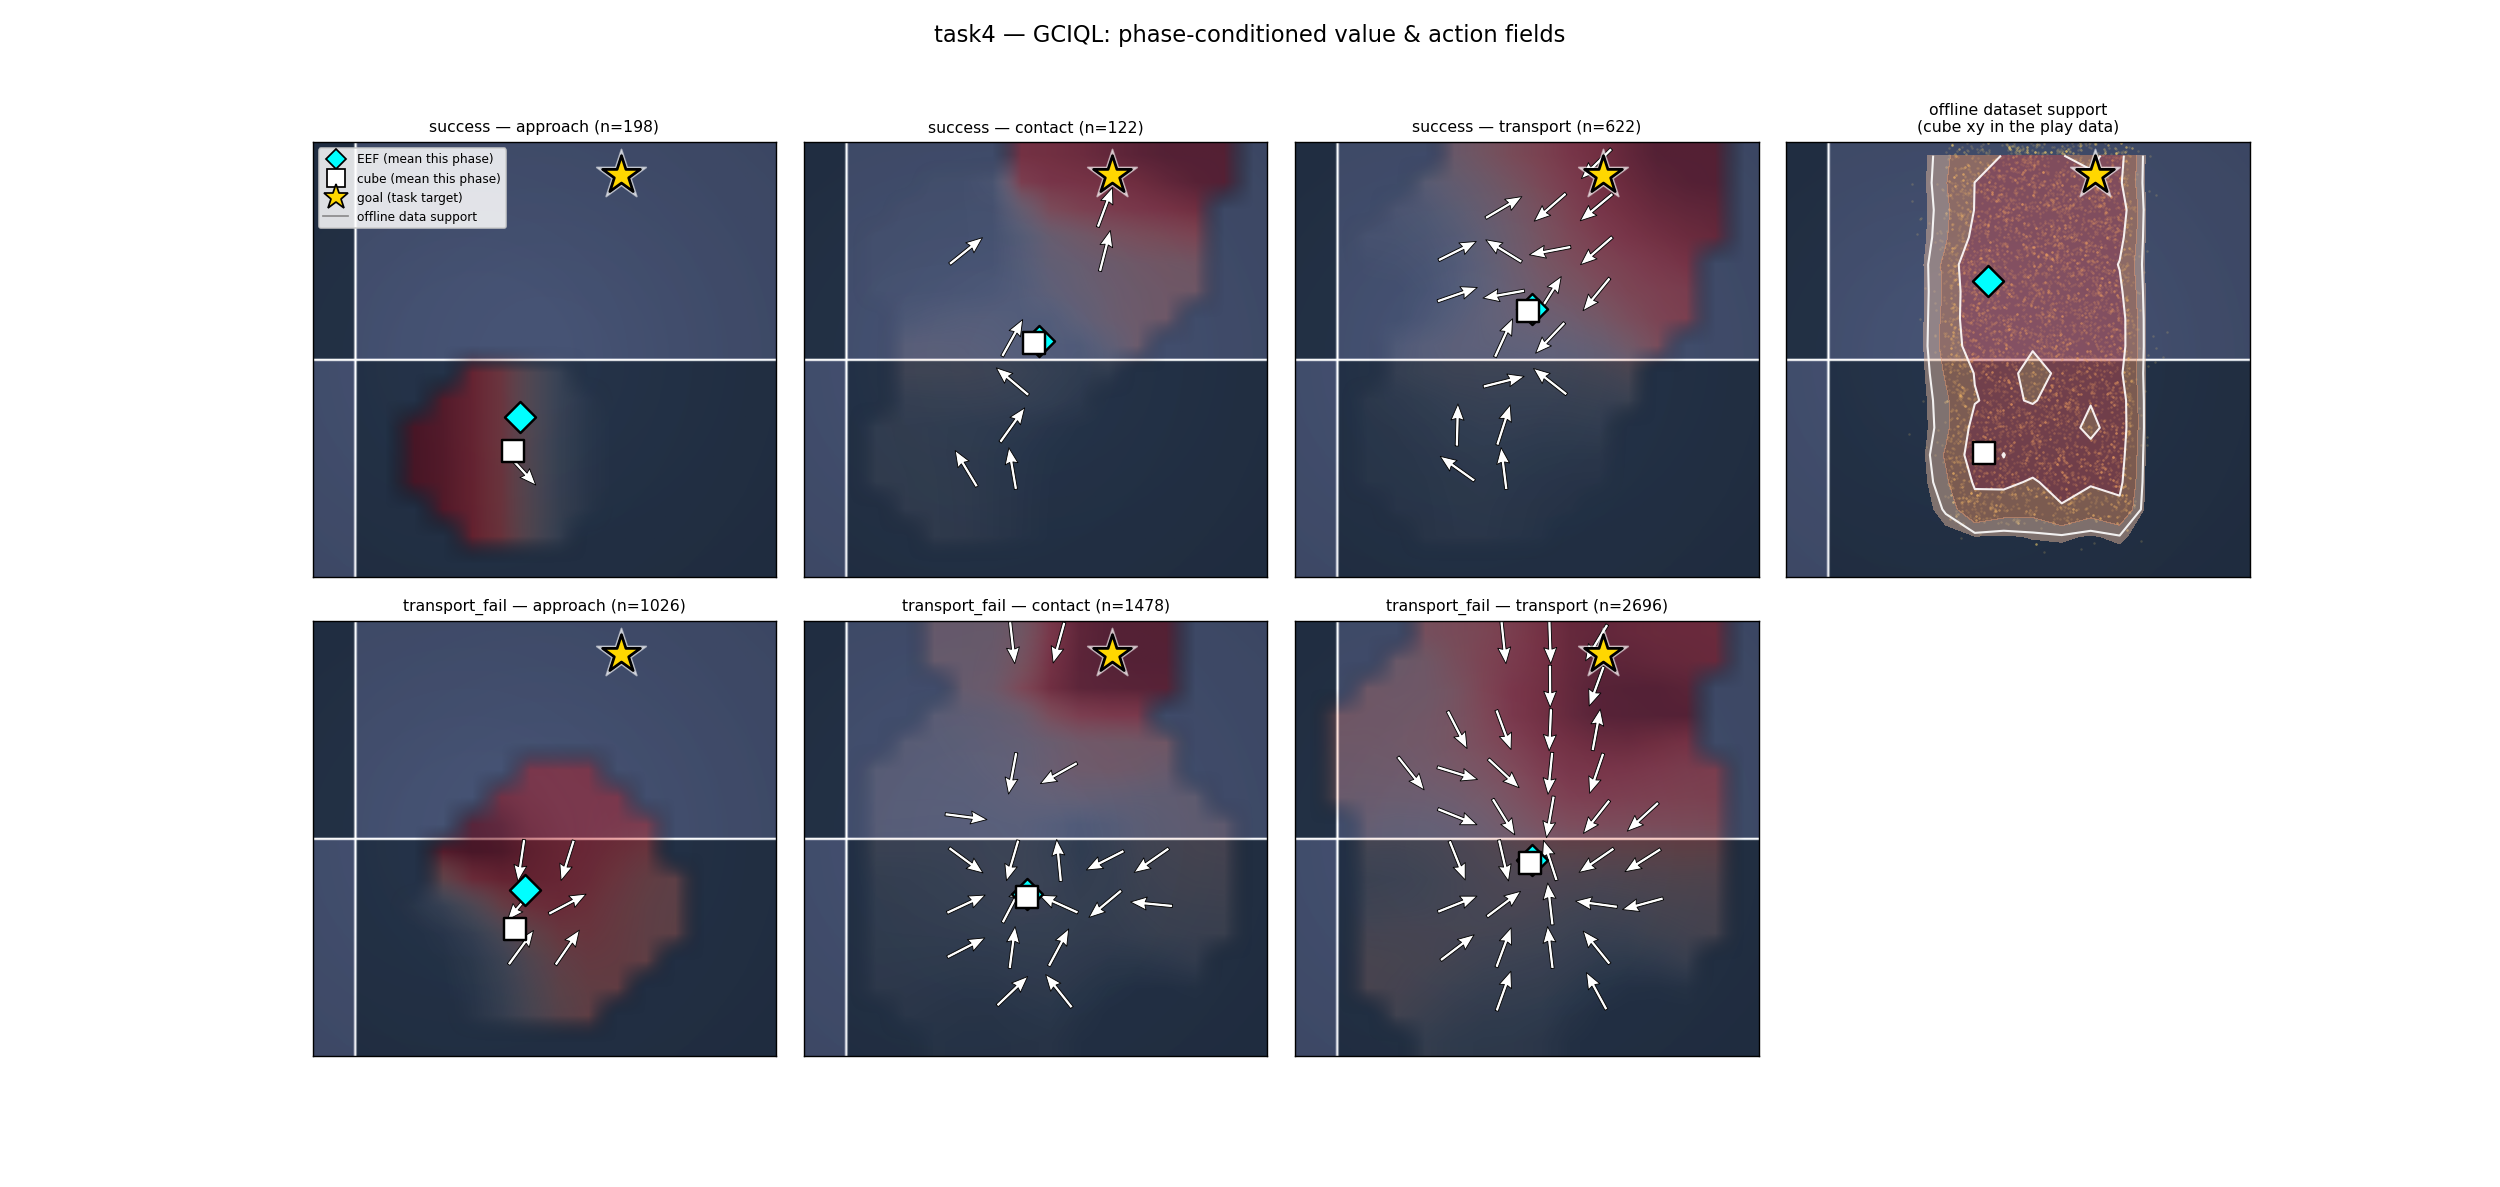
\includegraphics[width=\linewidth]{figures/pixel/pixel_phase_task4__GCIQL.png}
        \caption{task4 -- GCIQL.}
    \end{subfigure}
    \caption{Pixel observations: phase-conditioned value/action fields for task4.}
\end{figure}

\begin{figure}[H]
    \centering
    \begin{subfigure}{0.49\linewidth}
        \centering
        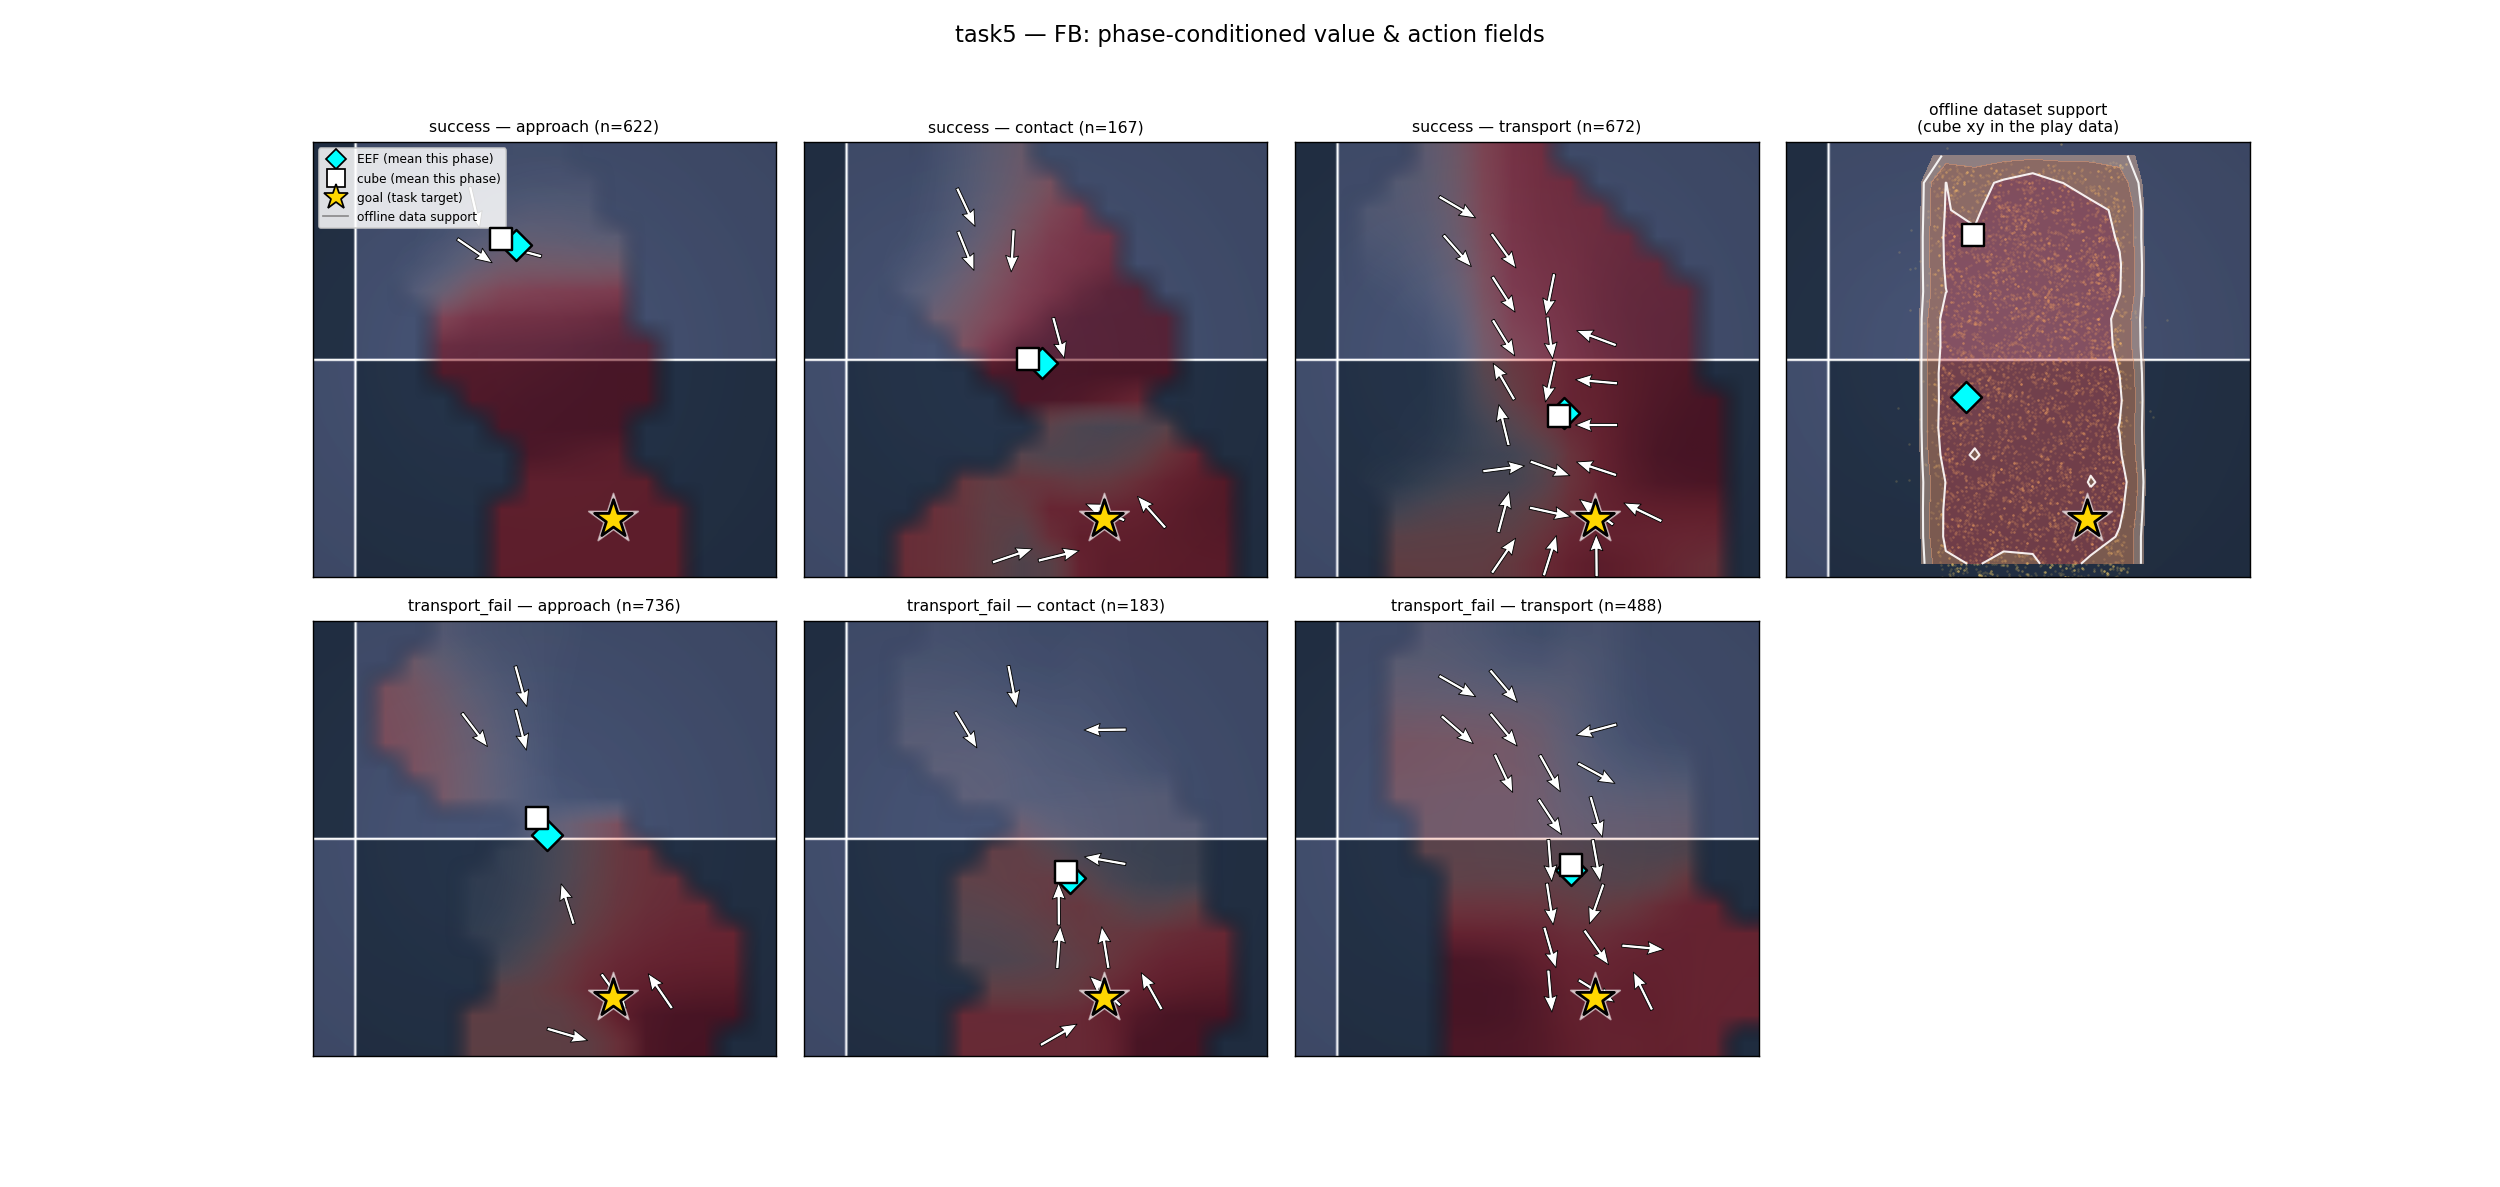
\includegraphics[width=\linewidth]{figures/pixel/pixel_phase_task5__FB.png}
        \caption{task5 -- FB.}
    \end{subfigure}\hfill
    \begin{subfigure}{0.49\linewidth}
        \centering
        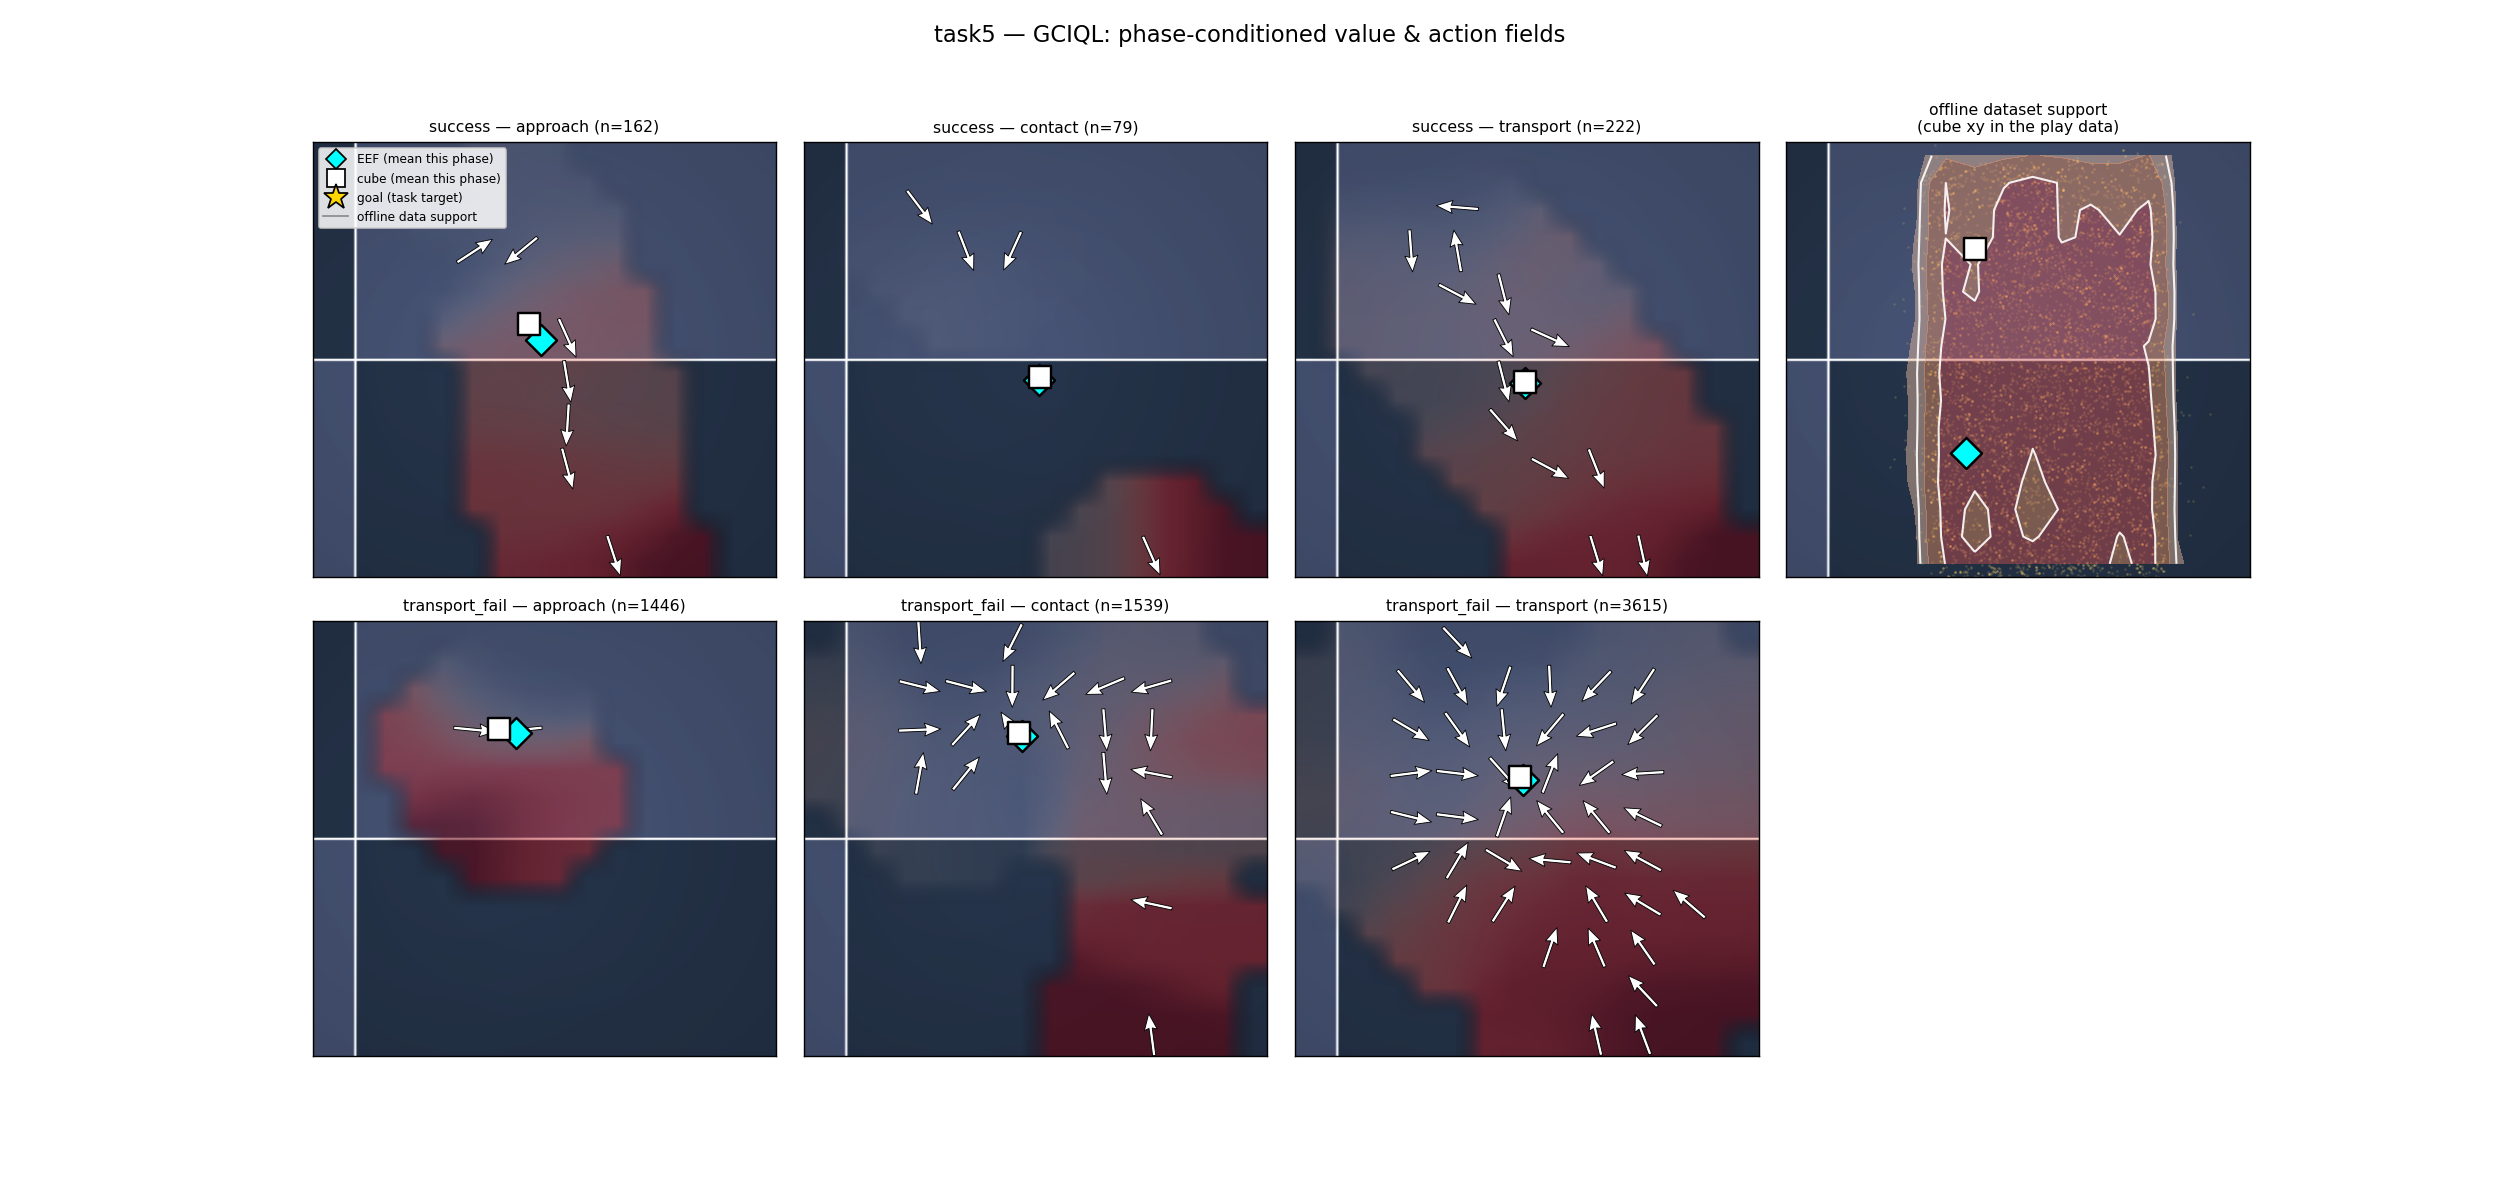
\includegraphics[width=\linewidth]{figures/pixel/pixel_phase_task5__GCIQL.png}
        \caption{task5 -- GCIQL.}
    \end{subfigure}
    \caption{Pixel observations: phase-conditioned value/action fields for task5.}
\end{figure}

\section{Cube-Position Coverage Construction}
\label{app:coverage-construction}

The cube-position coverage plot is constructed from three sources. First, training cube xy positions are extracted from the offline play-data buffer. The buffer's per-episode \texttt{.npz} files store a raw 21-dimensional \texttt{physics} array without an explicit cube-field label. We identify the cube-xy column pair by scanning consecutive two-column windows of \texttt{physics} and \texttt{observation}, then scoring each candidate against cube xy positions already recorded in greedy rollouts. The score combines axis-range overlap and binary occupancy IoU on a $24\times24$ grid. On the \texttt{cube-single-play} buffer, this selects \texttt{physics[:,14:16]}, which is read at each episode's first and last timestep to produce training cube-start and cube-end positions. Second, evaluation cube-start xy is extracted from the per-episode cube position at $t=0$ from each closed-loop greedy rollout, pooled across both methods, all seeds, all tasks, and all evaluation episodes. Third, evaluation task goals are read by resetting the environment with each \texttt{task\_id} and recording \texttt{cur\_task\_info["goal\_xyzs"]}.

\section{Architectures and Hyperparameters}
\label{app:hparams}

\paragraph{FB+FlowBC architecture.}
Our FB agent is a PyTorch port of the \texttt{metamotivo}/\texttt{td\_jepa} FB implementation. State observations use identity encoders. Pixel observations use separate DrQ-v2 convolutional encoders for the forward and backward branches. The actor is noise-conditioned and trained with a DDPG+BC-style loss: a deterministic policy-gradient term normalized by running $\overline{|Q|}$ plus a behavior-cloning term toward flow-generated samples.

\paragraph{GCIQL architecture.}
GCIQL is the goal-conditioned IQL baseline from the OGBench reference implementation. It learns a goal-conditioned value function, twin critic, and policy with hidden sizes $[512,512,512]$ and LayerNorm. The pixel variant prepends an IMPALA-small convolutional encoder with image augmentation.

\begin{table}[H]
\centering
\small
\caption{FB+FlowBC hyperparameters.}
\label{tab:fb-hparams}
\vspace{0.25em}
\begin{tabular}{lcc}
\toprule
\textbf{Hyperparameter} & \textbf{State} & \textbf{Pixel} \\
\midrule
Observation & state vector & $64\times64$ RGB, 3-frame stack \\
Task dimension $z$ & 50 & 50 \\
Left-encoder dim $L$ & 50 & 256 \\
Forward map (hidden, layers, embed, ensemble) & 512, 2, 2, 2 & 512, 2, 2, 2 \\
Backward map (hidden, layers, norm) & 512, 4, yes & 512, 4, yes \\
Actor (noise-cond.; hidden, layers, embed) & 512, 2, 2 & 512, 2, 2 \\
Flow steps & 10 & 10 \\
Discount $\gamma$ & 0.99 & 0.99 \\
LR ($F$, $B$, actor, flow) & 1e\text{-}4, 1e\text{-}4, 1e\text{-}4, 3e\text{-}4 & same \\
Ortho.\ coef.\ (on $B$) & 1000 & 1.0 \\
BC coef.\ & 3.0 & 3.0 \\
Target $\tau$ & 0.005 & 0.005 \\
RGB encoder & --- & DrQ, feature 256 \\
Batch size & 256 & 256 \\
Train steps & $10^6$ & $10^6$ \\
\bottomrule
\end{tabular}
\end{table}

\begin{table}[H]
\centering
\small
\caption{GCIQL hyperparameters, from the OGBench reference implementation.}
\label{tab:gciql-hparams}
\vspace{0.25em}
\begin{tabular}{lcc}
\toprule
\textbf{Hyperparameter} & \textbf{State} & \textbf{Pixel} \\
\midrule
Observation & state vector & $64\times64$ RGB \\
Value / critic hidden & [512, 512, 512] & [512, 512, 512] \\
Actor hidden & [512, 512, 512] & [512, 512, 512] \\
LayerNorm & yes & yes \\
Expectile & 0.9 & 0.9 \\
Actor loss / \texttt{alpha} & ddpgbc / 1.0 & ddpgbc / 1.0 \\
Discount $\gamma$ / target $\tau$ & 0.99 / 0.005 & 0.99 / 0.005 \\
Learning rate & 3e\text{-}4 & 3e\text{-}4 \\
Encoder & none & IMPALA-small \\
Image aug.\ prob. & 0.0 & 0.5 \\
Batch size & 1024 & 256 \\
Train steps & $10^6$ & $5\times10^5$ \\
\bottomrule
\end{tabular}
\end{table}

% \bibliographystyle{plainnat}
% \bibliography{../lib}

\end{document}
